% Customizable fields and text areas start with % >> below.
% Lines starting with the comment character (%) are normally removed before release outside the collaboration, but not those comments ending lines

% svn info. These are modified by svn at checkout time.
% The last version of these macros found before the maketitle will be the one on the front page,
% so only the main file is tracked.
% Do not edit by hand!
\RCS$Revision: 467423 $
\RCS$HeadURL: svn+ssh://tklijnsm@svn.cern.ch/reps/tdr2/notes/HIG-17-028/trunk/HIG-17-028.tex $
\RCS$Id: HIG-17-028.tex 467423 2018-07-04 21:35:20Z tulika $
%%%%%%%%%%%%% local definitions %%%%%%%%%%%%%%%%%%%%%
% This allows for switching between one column and two column (cms@external) layouts
% The widths should  be modified for your particular figures. You'll need additional copies if you have more than one standard figure size.
\newlength\cmsFigWidth
\ifthenelse{\boolean{cms@external}}{\setlength\cmsFigWidth{0.85\columnwidth}}{\setlength\cmsFigWidth{0.49\textwidth}}
\ifthenelse{\boolean{cms@external}}{\providecommand{\cmsLeft}{upper\xspace}}{\providecommand{\cmsLeft}{left\xspace}}
\ifthenelse{\boolean{cms@external}}{\providecommand{\cmsRight}{lower\xspace}}{\providecommand{\cmsRight}{right\xspace}}
%%%%%%%%%%%%%%%  Title page %%%%%%%%%%%%%%%%%%%%%%%%
\cmsNoteHeader{HIG-17-028} % This is over-written in the CMS environment: useful as preprint no. for export versions
% >> Title: please make sure that the non-TeX equivalent is in PDFTitle below
\title{Combined measurement and interpretation of differential Higgs boson production cross sections at $\sqrt{s}$=13 TeV}

% >> Authors
%Author is always "The CMS Collaboration" for PAS and papers, so author, etc, below will be ignored in those cases
%For multiple affiliations, create an address entry for the combination
%To mark authors as primary, use the \author* form
\author[cern]{The CMS Collaboration}

% >> Date
% The date is in yyyy/mm/dd format. Today has been
% redefined to match, but if the date needs to be fixed, please write it in this fashion.
% For papers and PAS, \today is taken as the date the head file (this one) was last modified according to svn: see the RCS Id string above.
% For the final version it is best to "touch" the head file to make sure it has the latest date.
\date{\today}

% >> Abstract
% Abstract processing:
% 1. **DO NOT use \include or \input** to include the abstract: our abstract extractor will not search through other files than this one.
% 2. **DO NOT use %**                  to comment out sections of the abstract: the extractor will still grab those lines (and they won't be comments any longer!).
% 3. For PASs: **DO NOT use tex macros**         in the abstract: CDS MathJax processor used on the abstract doesn't understand them _and_ will only look within $$. The abstracts for papers are hand formatted so macros are okay.
\abstract{The differential Higgs boson production cross sections are sensitive probes for new physics beyond the standard model. In particular, new physics may contribute in the gluon-gluon fusion loop, the dominant Higgs boson production mechanism at the LHC, and manifest itself as deviations from the expected standard model distributions. Combined spectra from the $H\to\gamma\gamma$, $H\to ZZ$ and $H\to b\bar{b}$ decay channels are presented, together with limits on the Higgs couplings using 35.9$\,$fb${}^{-1}$ of proton-proton collision data recorded with the CMS detector at $\sqrt{s}=13\,$TeV.}

% >> PDF Metadata
% Do not comment out the following hypersetup lines (metadata). They will disappear in NODRAFT mode and are needed by CDS.
% Also: make sure that the values of the metadata items are sensible and are in plain text:
% (1) no TeX! -- for \sqrt{s} use sqrt(s) -- this will show with extra quote marks in the draft version but is okay).
% (2) no %.
% (3) No curly braces {}.
\hypersetup{%
pdfauthor={M. Donega, T. Klijnsma, P. Musella},%
pdftitle={Combined measurement and interpretation of differential Higgs boson production cross sections at $\sqrt{s}$=13 TeV},%
pdfsubject={CMS},%
pdfkeywords={differential cross sections, combination, Higgs coupling modifiers}}

\maketitle %maketitle comes after all the front information has been supplied
% >> Text
%%%%%%%%%%%%%%%%%%%%%%%%%%%%%%%%  Begin text %%%%%%%%%%%%%%%%%%%%%%%%%%%%%
%% **DO NOT REMOVE THE BIBLIOGRAPHY** which is located before the appendix.
%% You can take the text between here and the bibiliography as an example which you should replace with the actual text of your document.
%% If you include other TeX files, be sure to use "\input{filename}" rather than "\input filename".
%% The latter works for you, but our parser looks for the braces and will break when uploading the document.
%%%%%%%%%%%%%%%

\newcommand{\cmsTopLeft}{top left\xspace}
\newcommand{\cmsTopRight}{top right\xspace}
\newcommand{\cmsBottomLeft}{bottom left\xspace}
\newcommand{\cmsBottomRight}{bottom right\xspace}

\newcommand{\hgg}{H\,\to\gamma\gamma}
\newcommand{\hzztofourl}{H\,\to ZZ \to4\ell}
\newcommand{\hzz}{H\,\to ZZ}
\newcommand{\hbb}{H\,\to b\bar{b}}
\newcommand{\BRgamgam}{\text{BR}_{\gamma\gamma}}
\newcommand{\BRZZ}{\text{BR}_{ZZ}}

% \newcommand{\pt}{p_\text{T}} % This is a standard one for CMS
\newcommand{\pth}{\pt^\text{H}}
\newcommand{\njets}{N_\text{jets}}
\newcommand{\absynoH}{\left|y\right|}
\newcommand{\absy}{\left|y_\text{H}\right|}
\newcommand{\ptjet}{\pt^\text{jet}}
\newcommand{\Emiss}{E_\text{T}^\text{miss}}

\newcommand{\msd}{m_\text{SD}}

\newcommand{\cg}{c_g}

\newcommand{\pb}{\,pb}
\newcommand{\ifb}{\,fb$^{-1}$ }


% To add clearpages before sections (for easier editing)

\newboolean{booleanclearpagetoggle}
\setboolean{booleanclearpagetoggle}{false}
\newcommand{\toggledclearpage}{\ifthenelse{\boolean{booleanclearpagetoggle}}{\clearpage}{} }

\newcommand{\tk}[1]{\textbf{\color{orange}  [#1 -- tk]}}
\newcommand{\pasq}[1]{\textbf{\color{green}  [#1 -- pm]}}
\newcommand{\md}[1]{\textbf{\color{red}  [#1 -- md]}}

\newcommand{\arc}[1]{
    \ifthenelse{\boolean{booleanclearpagetoggle}}{\textbf{\color{blue}  [#1 -- arc]}}{}
    }
\newcommand{\ccle}[1]{
    \ifthenelse{\boolean{booleanclearpagetoggle}}{\textbf{\color{red}  [#1 -- CCLE]}}{}
    }


% Results
% \newcommand{\kappacLeftAsimov}{-5.5}
% \newcommand{\kappacRightAsimov}{5.4}
% \newcommand{\kappacLeftObserved}{-4.2}
% \newcommand{\kappacRightObserved}{4.2}
% \newcommand{\kappabLeftAsimov}{-1.2}
% \newcommand{\kappabRightAsimov}{1.2}
% \newcommand{\kappabLeftObserved}{-0.9}
% \newcommand{\kappabRightObserved}{0.9}
\newcommand{\kappacLeftAsimov}{-5.4}
\newcommand{\kappacRightAsimov}{5.3}
\newcommand{\kappacLeftObserved}{-4.3}
\newcommand{\kappacRightObserved}{4.3}
\newcommand{\kappabLeftAsimov}{-1.2}
\newcommand{\kappabRightAsimov}{1.2}
\newcommand{\kappabLeftObserved}{-0.9}
\newcommand{\kappabRightObserved}{0.9}

\newcommand{\kappabLeftAsimovFLOATINGBRS}{-3.7}
\newcommand{\kappabRightAsimovFLOATINGBRS}{7.3}
\newcommand{\kappabLeftObservedFLOATINGBRS}{-2.8}
\newcommand{\kappabRightObservedFLOATINGBRS}{9.9}
\newcommand{\kappacLeftAsimovFLOATINGBRS}{-15.7}
\newcommand{\kappacRightAsimovFLOATINGBRS}{19.3}
\newcommand{\kappacLeftObservedFLOATINGBRS}{-18.0}
\newcommand{\kappacRightObservedFLOATINGBRS}{22.9}


% Writes a \clearpage for every \toggledclearpage
% Otherwise, \toggledclearpage does nothing
% \setboolean{booleanclearpagetoggle}{true}

% Let whether or not the ToC is generated also depend on this boolean
\ifthenelse{\boolean{booleanclearpagetoggle}}{\tableofcontents}{}
\toggledclearpage 

\toggledclearpage
\section{Introduction}
\label{sec:introduction}

The Higgs boson, whose existence is predicted by the Brout-Englert-Higgs mechanism~\cite{Higgs:1964pj,Englert:1964et,Guralnik:1964eu}, is responsible for electroweak symmetry breaking in the standard model (SM).
% 
Since its discovery~\cite{Aad:2012tfa,Chatrchyan:2012xdj} at the CERN LHC, extensive effort has been dedicated to the measurement of its properties and couplings.

% Measurements have been made of both differential and inclusive cross sections for Higgs boson production but most of the information about its properties has come from measurements of total yields~\cite{Khachatryan:2016vau,Aad:2015gba,Khachatryan:2014jba,ATLAS:2017ovn,CMS:2018lkl}, which have thus far been found to be consistent with SM predictions.
% % 
% In this analysis we study the differential cross sections for the Higgs boson, which enables measurements of deviations in differential distributions that are not accessible via an inclusive measurement.
% % 
% By varying the Higgs couplings, the strength with which quarks and other bosons couple to the Higgs boson, significant distortions in the shapes of differential cross sections appear, in particular for the transverse momentum distribution.
% % 
In this analysis we study the differential cross sections for the production of Higgs bosons. 
% 
Significant distortions of the shapes of differential cross sections appear when the Higgs couplings to quarks and to other bosons are varied.
% 
These distortions are particularly pronounced in the transverse momentum distribution.
% 
Measurements of differential distributions therefore provide information on the couplings that cannot be obtained from inclusive measurements~\cite{Khachatryan:2016vau,Aad:2015gba,Khachatryan:2014jba,ATLAS:2017ovn,CMS:2018lkl}.
% 
By fitting parametrized predicted spectra to a state-of-the-art combination of differential cross sections, one can constrain Higgs couplings.


While the couplings to the top ($y_t$) and bottom ($y_b$) quarks are known with fair precision, there is still a relatively large uncertainty on the couplings to lighter quarks such as the charm.
% 
Increasing the precision on the Higgs boson couplings can provide fundamental insight into the SM, as they are free parameters in the SM Lagrangian and are sensitive to a range of beyond the SM theories
~\cite{Dimopoulos:1981zb,Witten:1981nf}.
% 
A proof-of-concept study determining limits on the modification of the Higgs coupling to the charm quark $\kappa_c$ from the Higgs boson transverse momentum distribution was performed in Ref.~\cite{Bishara:2016jga}
% using ATLAS data from Run I,
using $20.3$\ifb of data collected by ATLAS at a centre-of-mass energy $\sqrt{s}=8$~\cite{Aad:2015lha},
yielding the overall bounds $\kappa_c \in [ -16, 18 ]$.
% 
Direct detection of $H \rightarrow J/\psi$, which relies on charm-tagging, leads to significantly weaker limits: A recent study from the ATLAS Collaboration~\cite{Aaboud:2018fhh} quotes an expected upper limit on $\sigma(pp\rightarrow ZH) \times \text{BR}(H\rightarrow cc)$ of $150^{+80}_{-40}$ times the SM value at 95\% CL, which corresponds to a limit about 4 times weaker.
% 
An analysis by the ATLAS Collaboration of $H \rightarrow J/\psi\gamma$~\cite{Aad:2015sda}, involving the detection of an associated photon, yields $\left|\kappa_c\right|<429$~\cite{Koenig:2015pha} at 95\% CL.
% 
Limits from detection of $pp \rightarrow VH(\rightarrow cc)$ at LHCb~\cite{LHCb:2016yxg} and $pp \rightarrow Hc$~\cite{Brivio:2015fxa} do not yield competitive limits at the current integrated luminosity, although projections to higher luminosities indicate they may do so in the future.
% 
% \arc{What are the physics model that could produce anomalous kc, kb, kt, kg ? It could be interesting to include some examples in the introduction.}
% 
% \tk{Postpone this comment}


Both the ATLAS and CMS Collaborations have reported measurements of differential cross sections at $\sqrt{s}=8$ and $13$\TeV~\cite{Aad:2014lwa,Khachatryan:2015rxa,Aad:2014tca,Khachatryan:2015yvw,Aad:2016lvc,Khachatryan:2016vnn,Aaboud:2017oem,CMS_AN_2016-442,ATLAS:2018uoi,Aaboud:2018xdt}.
% 
We report the measurements of differential cross sections obtained from a combination of results from the CMS Collaboration in the $\hgg$~\cite{CMS_AN_2017-299}, $\hzztofourl$~\cite{CMS_AN_2016-442} and $\hbb$~\cite{CMS_AN_2016-366} decay channels.
% 
The results of the individual decay channels were all obtained at $\sqrt{s}=13\,$TeV, using a data set corresponding to an integrated luminosity of about $35.9\,\text{fb}^{-1}$.
% 
The differential cross sections for the following observables are combined: the Higgs boson transverse momentum $\pth$, the number of reconstructed hadronic jets $\njets$, the Higgs boson rapidity $\absy$, and the transverse momentum of the leading jet $\ptjet$.
% 
Furthermore, we interpret the Higgs boson transverse momentum spectrum in terms of Higgs boson couplings.
% 
In order to take into account the many degrees of freedom offered by the Higgs coupling modifier framework~\cite{LHCHiggsCrossSectionWorkingGroup:2012nn}, multiple couplings are varied simultaneously.
% 
We present results obtained by varying simultaneously
% 
(i) the modifier of the Higgs coupling to the charm quark $\kappa_c$ and of the bottom quark $\kappa_b$,
% 
(ii) the modifier of the Higgs coupling to the top quark $\kappa_t$ and the coefficient $\cg$ of the anomalous direct coupling to the gluon in the heavy top mass limit,
% 
and (iii) $\kappa_t$ and $\kappa_b$.



\toggledclearpage
\section{The CMS detector}

% See more texts at https://twiki.cern.ch/twiki/bin/viewauth/CMS/Internal/PubDetector

The central feature of the CMS apparatus is a superconducting solenoid of 6\unit{m} internal diameter, providing a magnetic field of 3.8\unit{T}. Within the solenoid volume are a silicon pixel and strip tracker, a lead tungstate crystal electromagnetic calorimeter (ECAL), and a brass and scintillator hadron calorimeter (HCAL), each composed of a barrel and two endcap sections. Forward calorimeters extend the pseudorapidity coverage provided by the barrel and endcap detectors. Muons are detected in gas-ionization chambers embedded in the steel flux-return yoke outside the solenoid. In the barrel section of the ECAL, an energy resolution of about 1\% is achieved for unconverted or late-converting photons in the tens of GeV energy range. The remaining barrel photons have a resolution of about 1.3\% up to a pseudorapidity of $\abs{\eta} = 1$, rising to about 2.5\% at $\abs{\eta} = 1.4$. In the endcaps, the resolution of unconverted or late-converting photons is about 2.5\%, while the remaining endcap photons have a resolution between 3 and 4\%~\cite{CMS:EGM-14-001}. When combining information from the entire detector, the jet energy resolution amounts typically to 15\% at 10\GeV, 8\% at 100\GeV, and 4\% at 1\TeV, to be compared to about 40\%, 12\%, and 5\% obtained when the ECAL and HCAL calorimeters alone are used. A more detailed description of the CMS detector, together with a definition of the coordinate system used and the relevant kinematic variables, can be found in Ref.~\cite{Chatrchyan:2008zzk}.

\toggledclearpage
\section{Inputs to the combined analysis}

For all the measurements used as input to the combination ($\hgg$~\cite{CMS_AN_2017-299}, $\hzztofourl$~\cite{CMS_AN_2016-442} and boosted $\hbb$~\cite{CMS_AN_2016-366}), the data set corresponds to an integrated luminosity of about $35.9\,\text{fb}^{-1}$.
% 
% \arc{reference to CMS Note 2016/336 is not appropriate. It looks like arxiv:1709.05543. One should refer to the CMS publication. Can you explain in the paper why this Hbb measurement especially is good for your purpose, and not other CMS Hbb measurements ?}
% 
% For the $\hgg$ and $\hzz$ decay channels the gluon fusion production process dominates, whereas for $\hbb$ the dominant production process is associated vector boson production.
% 
% The Higgs bosons contributing to the boosted $\hbb$ result have high transverse momentum and therefore this result addresses a region of phase space in which the $\hgg$ and $\hzz$ results are least sensitive.
% 
% Including the boosted $\hbb$ result in the combination improves the precision at high transverse momentum, where there is limited data in the $\hgg$ and $\hzz$ channels.
% 
The $\hbb$ decay channel is only included in the combination of the Higgs boson transverse momentum spectrum, where it contributes to the measurements at the higher end of the spectrum ($\pth > 350$\GeV).
% 
It improves the precision in a region of phase space that is sensitive to effects that manifest themselves at high transverse momentum, and in which the data in the $\hgg$ and $\hzz$ decay channels are limited.
% 
% Including the boosted $\hbb$ result in the combination improves the precision in a region of phase space sensitive to effects that manifest themselves at high transverse momentum.
% 
% This process is only included in the Higgs boson transverse momentum spectrum, where it contributes to the measurements at the higher end of the spectrum ($\pth > 350$\GeV).
% 
% Its inclusion in the combination provides improved precision in a region of phase space that is crucial for sensitivity to effects that manifest at high transverse momentum, such as resolving the quark-loop in the gluon fusion production process.
% 
% The inclusion of $\hbb$ applies only for the Higgs transverse momentum spectrum, where $\hbb$ contributes to the measurements in the higher end of the spectrum ($\pth > 350$\GeV).
% 
Tables~\ref{tab:binningpth}, \ref{tab:binningnjets}, \ref{tab:binningabsy} and \ref{tab:binningptjet} show an overview of the bin boundaries used in the individual analyses.
% 
% \arc{It might be good to say that for gamma gamma and ZZ are targeting mainly gluon fusion, while usually bb is targeting VH; however this analysis is inclusive also in bb. It may be also good to explain briefly how are done the analyses.}


The SM prediction for the differential cross sections is simulated at next-to-leading order (NLO) in perturbative quantum chromodynamics (QCD) with $\MGvATNLO$~\cite{Alwall:2014hca} for each of the four dominant Higgs production modes: gluon-gluon fusion (ggH), vector boson fusion (VBF), associated production with a W/Z boson (VH), and associated production with a top quark-antiquark pair (ttH).
% 
Up to two additional jets in association with the Higgs boson are included in the simulation.
% 
Simulated events are interfaced to \PYTHIA~\cite{Sjostrand:2014zea} for parton showering and hadronization and the CUETP8M1~\cite{Skands:1695787} parameter set is applied to tune the underlying event.
% 
A weight is applied to simulated gluon fusion events to match the predictions from the {\textsc{nnlops}} program~\cite{Hamilton:2012np, Kardos:2014dua}.
% 
This weight depends on the Higgs boson transverse momentum $\pth$ and the number of jets in the event $\njets$.
% 
% On events simulated in the gluon fusion production mode a weight is applied according to Higgs transverse momentum $\pth$ and the number of jets in the event $\njets$, in order to match prediction from the NNLOPS program~\cite{Hamilton:2012np, Kardos:2014dua}.
% 
%% Sentence from Vittorio; not sure if relevant:
% The POWHEG NNLOPS program has the advantage of predicting at next-to-next-to-leading-order accuracy, both the differential cross section with respect to the QCD radiative effects and the normalization of the inclusive cross section~\cite{Hamilton:2013fea}.
% 
% \tk{Sentence from Vitt to include somehow:}
% % 
% The SM Higgs boson cross sections and branching fractions are taken from the LHC Higgs Cross Section Working Group recommendations~\cite{deFlorian:2016spz}.
% % 
% \tk{For HZZ, mention what was used for the $ZZ \rightarrow 4 \ell$ decays.}


Each of the analyses used as input to the combination uses a different fiducial space.
% 
% The input analyses are performed in different fiducial phase spaces.
% 
In the case of $\hgg$, the fiducial phase space is defined by requiring the leading photon transverse momentum over the diphoton mass to be greater than $1/3$ and the subleading photon transverse momentum over the diphoton mass to be greater than $1/4$.
% 
Furthermore, for each photon candidate the sum of the generator level transverse energy of stable particles contained in a cone of radius $\Delta R=0.3$ around the candidate is required to be less than 10\GeV, where $\Delta R$ is the angular separation between particles ($\Delta R = \sqrt{ (\Delta\eta)^2 + (\Delta\phi)^2 }$).
% 
% Furthermore,
% % $Iso_{gen}$, 
% the maximum of the generator level hadronic energy contained in a cone of radius $\Delta R=0.3$ around each photon candidate is required to be less than 10\GeV, where $\Delta R$ is the angular separation between particles ($\Delta R = \sqrt{ (\Delta\eta)^2 + (\Delta\phi)^2 }$).
% 
% 
In the case of $\hzz$, the 4-lepton mass is required to be greater than 70$\,$GeV, the leading Z-candidate mass must be greater than 40$\,$GeV, leptons must be separated in angular space by at least
$\Delta R > 0.02$.
% 
Furthermore, at least two leptons must have a transverse momentum greater than 10$\,$GeV and at least one greater than 20$\,$GeV.
% 
% \tk{start hbb}
% 
In the case of $\hbb$, the analysis strategy requires the presence of a single anti-$k_T$ jet with a cone size $R=0.8$, $\pt>450\,$GeV, and $\left|\eta\right|<2.5$.
% 
Soft and wide-angle radiation is removed using the soft drop mass algorithm~\cite{Dasgupta:2013ihk}\cite{Larkoski:2014wba}.
% 
The jet mass after application of the soft drop mass algorithm $\msd$ peaks at the Higgs mass in the case of signal events.
% 
Cuts on the dimensionless mass scale variable for QCD jets $\rho=\log\left(m_{\text{SD}}^2/\pt^2\right)$~\cite{Dasgupta:2013ihk}, which relates the jet transverse momentum to the jet mass, are used to avoid finite cone effects and the non-perturbative regime of the soft drop mass calculation.
% 
Events with isolated electrons, muons or taus with $\pt>10$\GeV and $\absynoH<2.5$ are vetoed in order to reduce the background from SM electroweak processes, and events with $\Emiss>140$\GeV are vetoed in order to reduce the background from top-antitop quark production.



There are minor differences amongst the individual analyses in Refs.~\cite{CMS_AN_2017-299,CMS_AN_2016-442,CMS_AN_2016-366} and the inputs we used for the combination of differential observables.
% 
For $\hgg$, an additional bin boundary in the $\pth$ spectrum is included at $600$\GeV.
% 
For $\hzz$, the bin boundaries in multiple spectra were modified to align them with those used in the $\hgg$ analysis.
% 
% Furthermore, the branching fractions of the Z boson into two leptons are fixed to their SM value in this combination, whereas in Ref.~\cite{CMS_AN_2016-442} they are allowed to float.
% 
Furthermore, the branching fractions of the two Z bosons to the various lepton configurations were fixed to their SM values, whereas in Ref.~\cite{CMS_AN_2016-442} these were allowed to float.
% 
% Finally, minor improvements on the background prediction related to the bin-to-bin correlations were carried out in Ref.~\cite{CMS_AN_2016-442}, which are not included in our results.
% 
For $\hbb$ the signal was split into two $\pt$-bins at generator level: the first with bin boundaries from $350$ to $600$\GeV and the second an overflow bin starting at $600$\GeV, which aligns with the bin boundaries of the other decay channels.
% 
The original binning at reconstructed level is merged into two bins, with bin boundaries from $450$ to $600$ and $600$ to $1000$\GeV, chosen so that the majority of signal events in a reconstructed bin originate from one generator-level bin.
% 
The redefinition of the reconstructed transverse momentum categories necessitated a re-evaluation of the background model, which was performed using the same procedure as in the original analysis.




% % 
% % \arc{it is not clear why just those two bins are kept, and why only the double b-tagger (which by the way deserves a description) is used. Is there no signal in the other bins / categories ?}
% % 
% The analysis makes use of the double-b tagger algorithm~\cite{CMS:2016jdj}, which is designed to identify the boosted $\hbb$ signal based on both the jet substructure and the b tagging information of the bottom-antibottom quark pair in the jet.
% % 
% Two double-b tagger~\cite{CMS:2016jdj} discriminator categories are employed, one being rich in signal (called the ``passing'' region) and the other deprived of signal events (called the ``'').
% % 
% The relation between the yields in these categories from the multijet QCD final state, the dominant background, is described with a set of polynomials taking $\rho$ and $\pt$ as input parameters.
% % 
% % \arc{explain which observable is fitted (soft drop mass). Also explain why a background polynomial discussion is needed here, is there any bias ? This whole discussion about bb needs better motivations for all the choices done.}
% % 
% Based on the outcome of the Fisher $\mathcal{F}$-test, it was determined that a polynomial of third order in $\rho$ and of first order in $\pt$ was sufficient, rather than a polynomial of second order in $\rho$ and of first order in $\pt$ as was determined for the individual analysis.
% % 
% \arc{the H->bb changes description in lines 115-122 is not terribly clear. The message may be that the reco pt categories were redefined to have just 2,  and in so doing you had to re-evaluate the polynomial for the background shape, but it doesn't get through clearly.}
% 
% 
% 
% The parameterization of the polynomial QCD transfer factor was changed to the Bernstein basis to ensure fit stability in the combination.
% 
% \tk{Original reply from Javier:
% \textit{The six original RECO pT bins are merged into two bins from 450-600 GeV and 600-1000 GeV. We split the ggF signal into two Higgs GEN pT bins (chosen so that the majority of each RECO pT bin is composed of a single GEN pT bin) of 375-600 GeV and 600-Inf (bin edges to be checked with Michael here). In order to make the two-bin fit more stable, the parameterization of the polynomial QCD transfer factor (from the failing double-b tag region to the passing double-b tag region) was changed to the Bernstein basis to enforce a positive definite transfer factor by construction. The Fisher F-test was repeated for the new fit configuration and it determined that a polynomial 3rd order in $\rho = log(m_{SD}^2/pT^2)$ and 1st order in pT was sufficient to fit the data (rather than 2nd order in rho and 1st order in pT).}
% }

% \tk{
%     TODO: Description per decay channel of the differences between the workspace for the individual analysis and the workspace for the combination. \\
%     % 
%     For $\hgg$:
%     \begin{itemize}
%         \item Bin boundary at 600\GeV in $\pth$ spectrum
%         \item Split between ggH and xH may lead to minor changes in the signal fits
%     \end{itemize}
%     % 
%     For $\hzz$:
%     % 
%     \begin{itemize}
%     \item \textit{In HZZ, we modified the bin boundaries in accordance with the combination. The other change is that we fix the ZZ->4e,4mu,2e2mu branching fractions to the SM, whereas in HIG-16-041 they were allowed to float independently (to be more model independent). I improved the uncertainty scheme on the ZZ background prediction for the N(jets) differential cross section measurement, adopting a Stewart-Tackmann approach. This is because we considered only $>=3$ jets in HIG-16-041 but now we have $>=4$. This actually made very little difference in the actual results.
%     }
%     \end{itemize}
%     % 
%     For $\hbb$ [Still awaiting reply from authors here]:
%     \begin{itemize}
%         \item Does main analysis have the differential result?
%         \item Bernstein polynomian for bkg?
%     \end{itemize}
%     }

\begin{table}[htbH]
\footnotesize
\begin{center}
\begin{tabular}{|l|c|c|c|c|c|c|c|c|c|}
\hline
Channel & \multicolumn{9}{l|}{$\pth$ bin boundaries (GeV)} \\
\hline
$\hgg$
    & [0, 15)    & [15, 30)   & [30, 45)   & [45, 80)        & [80, 120)
    & [120, 200) & [200, 350) & [350, 600) & [600, $\infty$)
    \\
\hline    
$\hzz$
    & [0, 15) & [15, 30) & \multicolumn{2}{c|}{[30, 80)}
    & \multicolumn{2}{c|}{[80, 200)} & \multicolumn{3}{c|}{[200, $\infty$)}
    \\
\hline
$\hbb$
    & \multicolumn{7}{c|}{} & [350, 600) & [600, $\infty$)
    \\
\hline
\end{tabular}
\end{center}
\caption{
    $\pth$ bin boundaries for the $\hgg$, $\hzz$ and $\hbb$ decay channels.
    }
\label{tab:binningpth}
\end{table}

\begin{table}[htbH]
\begin{center}
\begin{tabular}{|l|c|c|c|c|c|}
\hline
Channel & \multicolumn{5}{l|}{$\njets$ bin boundaries (\# of jets)} \\
\hline
$\hgg$ & 0 & 1 & 2 & 3 & $\ge$4 \\
\hline
$\hzz$ & 0 & 1 & 2 & \multicolumn{2}{c|}{$\ge$3} \\
\hline
\end{tabular}
\end{center}
\caption{
    $\njets$ bins for the $\hgg$ and the $\hzz$ decay channels.
    }
\label{tab:binningnjets}
\end{table}

\begin{table}[htbH]
\begin{center}
\begin{tabular}{|l|c|c|c|c|c|c|}
\hline
Channel & \multicolumn{6}{l|}{$\absy$ bin boundaries} \\
\hline
$\hgg$ & [0.0, 0.15) & [0.15, 0.30) & [0.30, 0.60) & [0.60, 0.90) & \multicolumn{2}{c|}{[0.90, 2.50]} \\
\hline
$\hzz$ & [0.0, 0.15) & [0.15, 0.30) & [0.30, 0.60) & [0.60, 0.90) & [0.90, 1.20) & [1.20, 2.50] \\
\hline
\end{tabular}
\end{center}
\caption{
    $\absy$ bins for the $\hgg$ and the $\hzz$ decay channels.
    }
\label{tab:binningabsy}
\end{table}

\begin{table}[h!]
\begin{center}
\begin{tabular}{|l|c|c|c|c|c|c|}
\hline
Channel & \multicolumn{6}{l|}{$\ptjet$ bin boundaries (GeV)} \\
\hline
$\hgg$ & [0, 30) & [30, 55) & [55, 95) & [95, 120) & [120, 200) & [200, $\infty$) \\
\hline
$\hzz$ & [0, 30) & [30, 55) & [55, 95) & \multicolumn{3}{c|}{ [95, $\infty$) } \\
\hline
\end{tabular}
\end{center}
\caption{
    $\ptjet$ bin boundaries for the $\hgg$ and the $\hzz$ decay channels.
    }
\label{tab:binningptjet}
\end{table}

\toggledclearpage
\section{Statistical analysis}
\label{sec:statisticalanalysis}

% \arc{section 4 seems to contain a lot of math that is not really specific of this article. Equation (1) and the accompanying description are useful to explain the efficiency matrix and treatment of the out-of-fiducial, but the rest of the math is not necessary, and so it feels a bit out of place since the rest of the article is rather terse on details. Maybe it would be better to keep the first formula, and rather describe the others with words, highlighting the ideas of the mathematical treatment. Also, the math spells out the dependency of the nuisances in some places, but not in other quantities that should also depend on nuisance parameters, which may be confusing.}

% Instead of fitting cross sections to data, it is instead opted to fit \textit{signal strengths} for the combination of differential observables.
% % 
% The detector acceptance is still fully modelled, which makes the procedure equivalent to an extrapolation to full phase space.
% % 
% The signal strength $\mu$ is defined as the modifier of the SM cross section $\sigma_\text{SM}$ needed to best fit the data:
% % 
% \begin{equation}
%     \sigma = \mu \cdot \sigma_\text{SM}
%     \,,
% \end{equation}
% % 
% where $\sigma$ is a cross section that fits best to some data.

The cross sections are extracted through a simultaneous extended maximum likelihood fit~\cite{Cowan:2010js} to the diphoton, four-lepton and the anti-$k_T$ jet mass spectra in all the analysis categories of $\hgg$, $\hzz$ and $\hbb$ respectively.
% 
Systematic uncertainties are implemented as nuisance parameters.


The number of expected signal events $n^\text{sig}$ in a given reconstructed bin $i$, given analysis category $k$ and given decay channel $m$ is given by:
% 
\begin{equation}
n_i^{\text{sig},\,km}(\vec{\Delta\sigma} | \vec{\theta})
= \sum_{j=1}^{n_b^\text{gen}}
    \Delta\sigma_j \cdot L(\vec{\theta})
    \cdot A_j^{km}(\vec{\theta}) \cdot \text{BR}^{m}(\vec{\theta})
    \cdot \varepsilon_{ji}^{km}(\vec{\theta})
    + n^{\text{OOA},\,km}_i(\vec{\theta})
\,,
\label{eq:nsig}
\end{equation}
% 
where:
% 
\begin{itemize}
\item $j$ is an index to bin $j$ at generator level
% , and $l$ an index to invariant mass bin $l$
% 
\item $n_b^\text{gen}$ is the number of kinematic bins at generator level, which is the same for all decay channels
% 
% \item $\vec{\mu} = (\mu_1, \dots, \mu_{n_b})$ is the set of signal strengths at generator level per kinematic bin%
% % 
% \footnote{
%     The signal strengths can be reinterpreted as cross sections by multiplication with the SM cross section $\sigma^\text{SM}$.
%     % 
%     The detector acceptance is still fully modelled, which makes the procedure equivalent to an extrapolation to full phase space.
%     }
% 
% \item $\mathcal{L}_i(\vec{\mu})$ is the contribution from the $i^\text{th}$ kinematic bin at generator level to the overall likelihood to find $\vec{\mu}$
% 
% \item $S^{l}_{i}$ is the number of signal events in kinematic bin $i$ and invariant mass bin $l$
% 
% \item $\sigma$ is the inclusive cross section, and $L$ is the integrated luminosity of the samples used in this analysis
% 
\item $\vec{\Delta\sigma}$ is the set of differential cross sections at generator level, and $L$ is the integrated luminosity of the samples used in this analysis.
% 
\item $A_j^{km}$ is the acceptance (fraction of the overall cross section) in reconstructed bin $j$, and $\text{BR}^m$ is the branching fraction of decay channel $m$.
% 
\item $\varepsilon_{ji}^{km}$ is the efficiency with which events originating from bin~$j$ are reconstructed in bin~$i$%
% , specific for category $k$ and decay channel $m$
.
Note that the corresponding matrix $\vec{\varepsilon}^{\,km}$ need not be square; the number of reconstructed bins may be smaller than the number of bins at generator level.
% 
% \item $f_l^{sig}$ is the fraction of events in the invariant mass bin $l$ (i.e. the invariant mass distribution of the signal in bin $l$)
% 
\item $n^{\text{OOA},\,km}_i $ is the number of events originating from outside the fiducial phase space reconstructed in bin $i$, specific for category $k$ and decay channel $m$.
% 
This contribution is roughly 1\% of the total yield for $\hgg$, and a negligible fraction for the other decay channels.
% 
% $f_l^\text{OOA}$ is the fraction thereof that is reconstructed in the $l^\text{th}$ invariant mass bin.
% 
\item $\vec{\theta}$ is the set of nuisance parameters.
\end{itemize}
% 
The summation and the efficiencies ensure that bin-to-bin migrations are taken into account, effectively allowing unfolding of the detector effects.
% 
% The recommendations in Ref.~\cite{Hansen:LShape} do not indicate a further need for regularization of the detector unfolding.
% 
Following the prescription in Ref.~\cite{Hansen:LShape}, we found that no regularization term was needed.





An extended likelihood function~\cite{Cowan:2010js} for a single decay channel $m$ is constructed:
% 
% \begin{equation}
\begin{align}
\begin{split}
% \mathcal{L}(\vec{\Delta\sigma} | \vec{\theta})
\mathcal{L}_m(\vec{\Delta\sigma} | \vec{\theta}) =
    % \prod_{m=1}^{n_c}
    \prod_{i=1}^{n_b^{\text{reco},\,m}}
    \prod_{k=1}^{n_\text{cat}^m}
    \prod_{l=1}^{n_\mathcal{O}^m}
        &
        \left(
        \text{pdf}_i^{\,km}(\mathcal{O}_l^m | \vec{\Delta\sigma}, \vec{\theta})
        \right)^{ N_\text{obs}^{iklm} }
        % \,
        \\
        & \quad \cdot
        \text{Poisson}\left(
            N_\text{obs}^{ikm}
            \, \left| \,
            n_i^{\text{sig},\,km}(\vec{\Delta\sigma} | \vec{\theta})
            + n^{\text{bkg},\,km}_i(\vec{\theta})
            \right)\right.
\,,
\label{eq:L_per_decaychannel}
\end{split}
\end{align}
% \end{equation}
% 
where:
% 
\begin{itemize}
% 
\item $\mathcal{O}^m$ is the observable, i.e. the diphoton, four-lepton or the anti-$k_T$ jet mass for the $\hgg$, $\hzz$ and $\hbb$ decay channels respectively,
% 
\item $n_b^{\text{reco},\,m}$ is the number of reconstructed bins,
$n_\text{cat}^m$ is the number of categories for the decay channel,
and $n_\mathcal{O}^m$ is the number of bins for observable $\mathcal{O}$,
% 
\item $N_\text{obs}^{iklm}$ is the number of observed events reconstructed in kinematic bin $i$, category $k$ and observable bin $l$,
% 
\item $n^{\text{bkg},\,km}_i$ is the number of expected background events,
% 
\item $\text{pdf}_i^{\,km}(\mathcal{O}_l | \vec{\Delta\sigma}, \vec{\theta})$ is the probability distribution function for the observable, based on the signal and background distributions of the observable.
% 
\end{itemize}
% 
In order to combine decay channels, the likelihood formulae for the individual decay channels are multiplied:
% 
\begin{equation}
\mathcal{L}(\vec{\Delta\sigma} | \vec{\theta})
= \prod_{m=1}^{n_c} \mathcal{L}_m(\vec{\Delta\sigma} | \vec{\theta})
    \,\cdot\,
    \text{pdf}(\vec{\theta})
\,,
\end{equation}
% 
where $n_c$ is the number of decay channels included in the combination, $\mathcal{L}_m$ is the likelihood formula from Eq.~\ref{eq:L_per_decaychannel} specific to decay channel $m$, and $\text{pdf}(\vec{\theta})$ is the probability distribution of the nuisance parameters.
% 
For the individual analyses, the number of categories, invariant mass bins and even the number of reconstructed bins may differ, although the number of bins at generator level and their bin boundaries need to be aligned between decay channels.
% 
Note that a single set of differential cross sections and nuisance parameters is applied to all decay channels simultaneously.


The test statistic $q$ is defined as:
% 
\begin{equation}
q(\vec{\Delta\sigma}) = -2 \cdot \ln \left(
    \frac{
        \mathcal{L}
            \left(
            \vec{\Delta\sigma} \left| \hat{\vec{\theta}}_{\vec{\Delta\sigma}}
            \right)\right.
        }{
        \mathcal{L}
            \left(
            \hat{\vec{\Delta\sigma}} \left| \hat{\vec{\theta}}
            \right)\right.
        }
\right)
\,.
\label{eq:TestStatisticQ}
\end{equation}
% 
% 
The quantities $\hat{\vec{\Delta\sigma}}$ and $\hat{\vec{\theta}}$ are the unconditional maximum likelihood estimates for the parameters $\vec{\Delta\sigma}$ and $\vec{\theta}$ respectively, while $\hat{\vec{\theta}}_{\vec{\Delta\sigma}}$ denotes the maximum like estimate for $\vec{\theta}$ conditional on the values of $\vec{\Delta\sigma}$.
% 
% where $\mathcal{L}$ is the fitted likelihood, the symbol $\hat{{}}$ indicates the variable is left floating in the fit, i.e. it was ``profiled'', and $\vec{\theta}$ is the set of all nuisance parameters included in the likelihood fit.
% 
% $\hat{\theta}_\vec{\Delta\sigma}$ carries the subscript ``$\vec{\Delta\sigma}$'' to indicate it was optimized for fixed values of $\vec{\Delta\sigma}$.
% 
% In the limit of large statistics, $q$ is $\chi^2$-distributed.
% 
It is assumed that $q$ is $\chi^2$-distributed.
% 
% The uncertainties on the signal strengths are obtained by scanning $q$ over a range of values for some $\mu$, and recording the interval between the points where $q(\mu) = 1$.

The Higgs coupling modifiers are fitted through a largely analogous procedure, utilizing the full likelihood.
% 
The difference is that instead of freely floating parameters for the differential cross sections $\vec{\Delta\sigma}$, the differential cross sections are replaced with parametrizations of the theoretical spectra described in Sec.~\ref{sec:theory}:
% 
\begin{equation}
    \vec{\Delta\sigma} \; \to \; \vec{\Delta\sigma}( \kappa_a, \kappa_b )
    \,,
\end{equation}
% 
where $\kappa_a$ and $\kappa_b$ are the coupling modifiers to be fitted.
% 
The theoretical uncertainties described in Sec.~\ref{sec:theory} are implemented as nuisance parameters.
% 
The coupling modifiers are implemented as freely floating parameters in the fit, and as such the corresponding degree of freedom of $q$ is equal to the number of coupling modifiers.





% ____________________________________________________________________________
% ____________________________________________________________________________
%                Worked out signal and bkg distributions; drop

% % 
% % In a single bin of the invariant mass spectrum the expected number of signal events is given by:
% % 
% The density of signal events with respect to an observable $\mathcal{O}$ is given by:
% % 
% \begin{equation}
% \begin{align}
% % S^{l}_{i}(\vec{\mu} | \vec{\theta})
% S^{km}_{i}( \mathcal{O} | \vec{\Delta\sigma}, \vec{\theta})
% =
%     \sum_{j=1}^{n_b^\text{gen}}
%         \Delta\sigma_j \cdot L
%         \cdot A_j^{km} \cdot \text{BR}^{m}
%         \cdot \varepsilon_{ji}^{km}(\vec{\theta})
%         \cdot f_{j}^{\text{sig},\,km}( \mathcal{O} | \vec{\theta} )
%     + n^{\text{OOA},\,km}_i
%         \cdot f^{\text{OOA},\,km}( \mathcal{O} | \vec{\theta} )
% \,,
% %
% \label{eq:Ssig}
% \end{align}
% \end{equation}
% % 
% where:
% % 
% \begin{itemize}
% \item $\mathcal{O}$ is the observable that is fitted to (the invariant mass of the decay products for $\hgg$ and $\hzz$, and the soft-drop mass for $\hbb$).
% % 
% \item $S^{km}_{i}( \mathcal{O} | \vec{\Delta\sigma}, \vec{\theta})$ is the density of signal events with respect to observable $\mathcal{O}$ in reconstructed bin $i$.
% % 
% % \item $f_{j}^{\text{sig},\,km}(\mathcal{O},\vec{\theta})$ is the $l^\text{th}$ bin of the invariant (soft-drop) mass distribution of the signal in bin $j$.
% % 
% \item $f_{j}^{\text{sig},\,km}(\mathcal{O},\vec{\theta})$ is the signal distribution of events in observable $\mathcal{O}$ in bin $j$.
% % 
% \item $n^{\text{OOA},\,km}_i$ is the number of events reconstructed in bin $i$ originating from outside the fiducial phase space, and $f^{\text{OOA},\,km}( \mathcal{O} | \vec{\theta} )$ is the distribution thereof in observable $\mathcal{O}$.
% % 
% \end{itemize}
% % 
% % Equation~\ref{eq:Ssig} describes the invariant mass distribution, whereas Eq.~\ref{eq:nsig} describes the overall number of signal events.
% % 
% Equation~\ref{eq:Ssig} describes the density of signal events at a given value of $\mathcal{O}$, whereas Eq.~\ref{eq:nsig} describes the overall number of signal events.
% % 
% % Similarly, the number of background events in a given bin of the invariant mass distribution is given by:
% % 
% Similarly, the density of background events at a given value of $\mathcal{O}$ is given by:
% % 
% \begin{equation}
% \begin{align}
% B^{km}_i(\mathcal{O}|\vec{\theta})
% = n^{\text{bkg},\,km}_i
%     \cdot f^{\text{bkg},\,km}(\mathcal{O}|\vec{\theta})
% \,,
% \end{align}    
% \end{equation}
% % 
% where
% % $B^{km}_i(\mathcal{O}|\vec{\theta})$ is the density of expected background events in reconstructed bin $i$,
% $n^{\text{bkg},\,km}_i$ the number of background events, and $f^{\text{bkg},\,km}(\mathcal{O}|\vec{\theta})$ the distribution thereof.
% % 


%%%%%% Additional: worked out pdf(...)

% An overall probability distribution function of observable $\mathcal{O}$ may be constructed by summation of the signal and background distributions, and normalizing to one:
% % 
% \begin{equation}
% \text{pdf}_i^{\,km}(\mathcal{O} | \vec{\Delta\sigma}, \vec{\theta})
% = \frac{
%         % n_i^{\text{sig},\,km}(\vec{\Delta\sigma} | \vec{\theta}) \,
%         S^{km}_{i}( \mathcal{O} | \vec{\Delta\sigma}, \vec{\theta})
%         +
%         % n^{\text{bkg},\,km}_i
%         B^{km}_i(\mathcal{O}|\vec{\theta})
%     }{
%         n_i^{\text{sig},\,km}(\vec{\Delta\sigma} | \vec{\theta}) \,
%         + n^{\text{bkg},\,km}_i
%     }
% \,,
% \end{equation}
% % 
% where $\text{pdf}_i^{\,km}(\mathcal{O} | \vec{\Delta\sigma}, \vec{\theta})$ describes the probability to find an event measuring observable $\mathcal{O}$ in reconstructed bin $i$.


%                END OF Worked out signal and bkg distributions; drop
% ____________________________________________________________________________
% ____________________________________________________________________________

\toggledclearpage
\section{Theoretical predictions}
\label{sec:theory}

% \arc{Section 5: It's not too clear which model is used in which context, etc. At the moment this section is a bit confusing.}

% \arc{section 5 should spell out what's done for the branching fractions and non-ggH production modes.}

Differential cross sections may be used constrain physical parameters.
% 
In the case of Higgs boson production through gluon fusion, finite quark mass effects and moderate variations to Higgs couplings may manifest in distortions of the $\pth$ spectrum.
% 
We interpret the $\pth$ spectrum for gluon fusion in terms of modifications of the couplings of the Higgs boson using two models: one tailored to heavy quarks and thus sensitive to effects at high $\pt$~\cite{Grazzini:2017szg}, and the other considering the effect of lighter quarks in the gluon fusion loop~\cite{Bishara:2016jga}.
% 
Higgs boson production in association with bottom and top quarks is taken to scale quadratically with $\kappa_b$ and $\kappa_t$ respectively.
% 
The other production processes are taken to be independent of these couplings.
% 
The coupling modifiers are described within the context of the kappa-framework~\cite{LHCHiggsCrossSectionWorkingGroup:2012nn,Khachatryan:2016vau}:
% 
\begin{equation}
    \kappa_i^2
        = \frac{y_i}{y_i^\text{SM}}
        % = \frac{\sigma_i}{\sigma_i^\text{SM}}
    \,,
\end{equation}
% 
% where $\sigma_i$ is the production cross section of a Higgs boson resulting from the direct coupling to particle $i$.
% 
where $y_i$ is the Higgs boson coupling to particle $i$.
% 
The SM value of any $\kappa_i$ is equal to 1.


Recent developments in transverse momentum resummation procedures have allowed more accurate calculations of the $\pth$ spectrum when including the effects of lighter quarks on Higgs production through gluon fusion~\cite{Banfi:2013eda,Bozzi:2003jy,Becher:2010tm,Monni:2016ktx}.
% 
The $\pth$ spectrum for gluon fusion has been calculated for simultaneous variations of $\kappa_c$ and $\kappa_b$~\cite{Bishara:2016jga}, providing a novel approach to constrain these couplings via the $\pth$ spectrum.
% 
The variations are computed in Ref.~\cite{Bishara:2016jga} and we parameterize these with a quadratic polynomial for each bin of the differential production cross section, including an inhomogeneity due to the interference of the top quark with the bottom and charm quarks.
% 
The Higgs coupling to the top quark is fixed to its SM value in this model.
% 
% We parametrize these variations, taken precomputed as input from Ref.~\cite{Bishara:2016jga}, using a quadratic polynomial for each bin of the differential production cross section, including an inhomogeneity due to the interference of the top quark, whose coupling is fixed to its SM value in this model.
% 
% \arc{you mention coupling to top quark fixed to its SM value, and then introduce kt. This is contradictory, please specify in which case.}


A second model producing simultaneous variations of $\kappa_t$, $\cg$ and $\kappa_b$ by adding dimension-6 operators to the SM Lagrangian was built in Ref.~\cite{Grazzini:2017szg}.
% 
This study employs an analytic resummation performed up to next-to-next-to-leading logarithmic (NNLL) order for the lower $\pth$ region in order to obtain the $\pth$ spectrum at NNLO+NNLL accuracy.
% 
The dimension-6 operator whose coefficient is $\cg$ yields a direct coupling of the Higgs boson to the gluon, whose tensor structure corresponds to the heavy top mass limit.
% 
The derivation of $\cg$ is given in Ref.~\cite{Grazzini:2017szg} and the inclusive cross section is given by $\sigma \simeq \left| 12\cg + \kappa_t \right|^2 \sigma^\text{SM}$.
% 
% $\cg$ is defined according to the derivations described in Ref.~\cite{Grazzini:2017szg}, which yields a dependence of the inclusive cross section $\sigma \simeq \left| 12\cg + \kappa_t \right|^2 \sigma^\text{SM}$.
% 
Two other operators are included to describe modifications of $\kappa_t$ and $\kappa_b$.
% 
While the model allows simultaneous variation of all three coupling modifiers, we consider only simultaneous variations of $\kappa_t$ and $\cg$, and of $\kappa_t$ and $\kappa_b$.
% 
The precomputed spectra are taken as input from Ref.~\cite{Grazzini:2017szg} and are parametrized using a quadratic polynomial, neglecting the interference of the bottom and top quark in the gluon fusion loop.
% 
% In the case of differential cross sections, each cross section per bin has one parametrization.


% In order to map the finely binned theoretical predictions to the experimental binning, the theoretical spectrum is integrated within experimental bin boundaries.


The coupling modifiers affect not only the production cross section of the Higgs boson, but its branching fractions as well.
% 
Throughout our results we will consider the branching fractions to be scaling with the Higgs coupling modifiers.


\toggledclearpage
\section{Systematic uncertainties}
\label{sec:systematics}

The systematic experimental uncertainties from the input analyses are incorporated in the combination as nuisance parameters in the extended likelihood fit and are profiled.
% 
Among the decay channels, correlations are taken into account for the systematic uncertainties in jet energy scale and resolution, and integrated luminosity.
% 
Full descriptions of the experimental systematic uncertainties per decay channel may be found in Refs.~\cite{CMS_AN_2017-299,CMS_AN_2016-442,CMS_AN_2016-366}.

% \ccle{
%     Para starting L196. I don't think fiducial is being used quite correctly here. We tend to use it to mean a limited phase space but it means a benchmark. In this paragraph I think you are using it to describe a part of the whole phase space. I'd suggest revising to something like
%     "Our measurement is made over the full phase space rather than limited to a region of phase space. This means that uncertainties in the acceptances for the individual analyses and in the branching fractions may affect our results. The effect of the acceptance uncertainties per bin on the overall uncertainty is less than one percent and so this is neglected in the combination.
%     }

Our measurement is made for the full phase space rather than limited to a fiducial phase space (as is the case for the original $\hgg$ and $\hzz$ analyses).
% 
This means that uncertainties in the acceptances for the individual analyses and in the branching fractions may affect our results.
% 
The effect of the acceptance uncertainties per bin on the overall uncertainty is less than one percent and so this is neglected in the combination.
% 
% As our measurement covers the full phase space rather than a fiducial one (as is the case for the original $\hgg$ and $\hzz$ analyses), uncertainties related to the fiducial acceptance and the branching fractions in principle affect our results.
% % 
% The effect of the fiducial acceptance uncertainties per bin on the overall uncertainty was below one percent, and we have therefore neglected it in the combination.
% 
Likewise the overall effect of the branching fraction uncertainties on the combined spectra is below one percent, and has been neglected.
% 
The uncertainty in the inclusive production cross section from non-gluon fusion production modes, determined to be about 2.1\%~\cite{deFlorian:2016spz}, has been taken into account as a nuisance parameter.
% 
% \tk{Proofs for these statements to be included in the AN.}
% 
% \tk{Uncertainties related to fiducial acceptance and BR to be implemented and then described here.}
% 
% \arc{the placeholder for the uncertainties on the extrapolation to the full phase space should probably go under 6.2 theoretical uncertainties instead of 6.1 experimental uncertainties (or the subsectioning of section 6 could be dropped)}


The theoretical predictions described in Sec.~\ref{sec:theory} are subject to theoretical uncertainties from the renormalisation scale $\mu_R$, the factorisation scale $\mu_F$ and the resummation scale $Q$.
% 
The standard approach to evaluate the impact of these uncertainties is to compute an envelope of scale variations, and taking the extrema of the envelope.
% 
To this end, $\mu_R$ and $\mu_F$ are independently varied between $0.5$, $1$ and $2$ times their nominal value, whereas the fraction $\frac{\mu_R}{\mu_F}$ is not to be less than $0.5$ or greater than $2.0$.
% 
As the theoretical spectra in the $\kappa_t$/$\cg$/$\kappa_b$ case and the $\kappa_c$/$\kappa_b$ case contain a resummation, the resummation scale $Q$ is varied from $0.5$ to $2$ times its central value (while keeping $\mu_F$ and $\mu_R$ at their central value).
% 
The theoretical uncertainties are determined by applying the default approach of taking the minimum and maximum scale variations per bin.
% 
The resulting uncertainties are shown in Table~\ref{tab:TheoryUncertainties_kappab_kappac} for the $\kappa_b$/$\kappa_c$ spectra and in Table~\ref{tab:TheoryUncertainties_kappat_kappag} for the $\kappa_t$/$\cg$ spectra.
% 

\begin{table}[htb]
\footnotesize
\begin{center}
\begin{tabular}{lccccc}
\hline
% Generated on 18-05-04 16:59:22 by differentials/theory/scalecorrelation.py; current git commit: e4def5d final versions of fermilab plots
Bin boundaries (GeV) & [0, 15) & [15, 30) & [30, 45) & [45, 80) & [80, 120) \\
$\Delta^\text{scale}$ (\%) & 8.9\% & 6.6\% & 18.1\% & 22.0\% & 21.6\% \\
\hline
\end{tabular}
\end{center}
\caption{
    Theoretical uncertainties for the $\kappa_b$/$\kappa_c$ spectra.
    }
\label{tab:TheoryUncertainties_kappab_kappac}
\end{table}

\begin{table}[htb]
\footnotesize
\begin{center}
% \hspace*{-1.7cm}%
\setlength{\tabcolsep}{2pt}
\begin{tabular}{lccccccccc}
\hline
% Generated on 18-05-04 16:59:21 by differentials/theory/scalecorrelation.py; current git commit: e4def5d final versions of fermilab plots
Bin boundaries (GeV) & [0, 15) & [15, 30) & [30, 45) & [45, 80) & [80, 120) & [120, 200) & [200, 350) & [350, 600) & [600, 800) \\
$\Delta^\text{scale}$ (\%) & 12.7\% & 7.4\% & 9.5\% & 12.8\% & 17.4\% & 19.3\% & 20.9\% & 23.4\% & 8.2\% \\
\hline
\end{tabular}
\end{center}
\caption{
    Theoretical uncertainties for the $\kappa_t$/$\cg$ and $\kappa_t$/$\kappa_b$ spectra.
    % 
    % \tk{Need to make these tables fit to the page.}
    % 
    % \tk{
    %     Theory uncertainty tables necessary? If so I will make the tables prettier.
    %     % 
    %     Alternatively I only supply the covariance matrix.
    %     }
    }
\label{tab:TheoryUncertainties_kappat_kappag}
\end{table}



Theoretical uncertainties are subject to bin-to-bin correlations, that are notoriously difficult to calculate.
% 
We adopt a procedure that obtains a correlation coefficient directly from the individual scale variations:
% ~\cite{Grazzini:PrivateComm}:
% 
\begin{equation}
\rho = 
\frac{
    \sum_i ( \sigma_{1, i} - \overline{\sigma}_1 ) ( \sigma_{2, i} - \overline{\sigma}_2 )
    }{
    \sqrt{
        \sum_i ( \sigma_{1, i} - \overline{\sigma}_1 )^2
        \sum_i ( \sigma_{2, i} - \overline{\sigma}_2 )^2
        }
    }
    \,,
\end{equation}
% 
where $\sigma_{1 (2), i}$ is the cross section in bin 1 (2) of the $i^\text{th}$ scale variation, $\overline{\sigma}_{1 (2)}$ is the mean cross section in bin 1 (2), and $\rho$ is the resulting correlation coefficient between bin 1 and 2.
% 
% This method does not take into account correlations due to the uncertainties on the parton density functions (PDF).
% 
% \arc{Equation 10: it could be good to mention that bin by bin pdf uncertainty is neglected. Do you have a reference for “notoriously difficult to perform” ? Is the procedure that you use new ?}
% 
The correlation structure is characterized by strong correlations among the central bins.
% 
Only the bins below $15$\GeV and above $600$\GeV in $\pth$ are anti-correlated with the central region.

% The correlation matrices obtained from this procedure are shown in Fig.~\ref{fig:scalecorrelationmatrices}.
% % 
% % \tk{Supply plotted correlation matrices here? Note no CMS data is used for these plots.}
% % 
% % Since the theoretical calculations use different methods for modification of the SM Lagrangian, the correlation matrices are not expected to be the same \tk{Check this sentence}.
% % 
% In both cases the low $\pth$-region is less correlated with other bins than the other bins among one another.
% % 
% This is mostly due to the resummation that has a large impact on the low $\pth$-region.
% % 
% In the case of $\kappa_t$/$\cg$ variations, the overflow bin is less correlated as well.

% \begin{figure}[hbtp]
%   \begin{center}
%     \includegraphics[width=\cmsFigWidth]{img/corrmats_newbinning/corrmat_yukawa.pdf}
%     \includegraphics[width=\cmsFigWidth]{img/corrmats_newbinning/corrmat_tophighpt.pdf}
%     \caption{
%         (\cmsLeft) Correlation matrix for theoretical uncertainties on $\kappa_b$/$\kappa_c$ variations.
%         (\cmsRight) Correlation matrix for theoretical uncertainties on $\kappa_t$/$\cg$/$\kappa_b$ variations.
%         % 
%         % \tk{Add ``CMS Preliminary 35.9 fb$^{-1}$'' here? It's not a plot that uses CMS data.}
%         }
%     \label{fig:scalecorrelationmatrices}
%   \end{center}
% \end{figure}



\toggledclearpage
\section{Results}

% ____________________________________________________________________________
\subsection{Total cross section and \texorpdfstring{$\BRgamgam/\BRZZ$}{BRgg/BRZZ}}
\label{sec:ratioOfBrsTotalXS}

% hgg:  63.9682042688 +- 9.59143702402
% hzz:  58.2260927627 +- 9.84281414263
% comb: 61.1477521912 +- 7.059056068

The total cross section for Higgs production is measured to be
$61.1   \pm 6.0 \,\text{(stat.)}   \pm 3.7 \,\text{(syst.)}  $\pb
, based on a combination of the total cross sections from $\hgg$ ($64.0\pm9.6$\pb)
and $\hzz$ ($58.2\pm9.8$\pb).
% 
The likelihood scans for the individual decay channels and their combination is shown in
Fig.~\ref{fig:RatioOfbrsAndTotalXSscan}~(\cmsLeft).
% 
The combination result agrees with the current SM value of $55.6\pm2.5$\pb~\cite{deFlorian:2016spz}.

A measurement of the branching fraction of one decay channel is degenerate with a measurement of the total cross section.
% 
However, the ratio of branching fractions for two decay channels can be measured while profiling the total cross section.
% 
The ratio of the $\hgg$ and $\hzz$ branching fractions $R$ is measured to be
$0.092   \pm 0.018 \,\text{(stat.)}   \pm 0.010 \,\text{(syst.)}  $, based on a combination of $\hgg$ and $\hzz$.
% 
This is in agreement with the SM prediction of $0.086$~\cite{deFlorian:2016spz}.
% 
The likelihood scan for $R$ is shown in Fig.~\ref{fig:RatioOfbrsAndTotalXSscan}~(\cmsRight).

\begin{figure}[hbtp]
  \begin{center}
    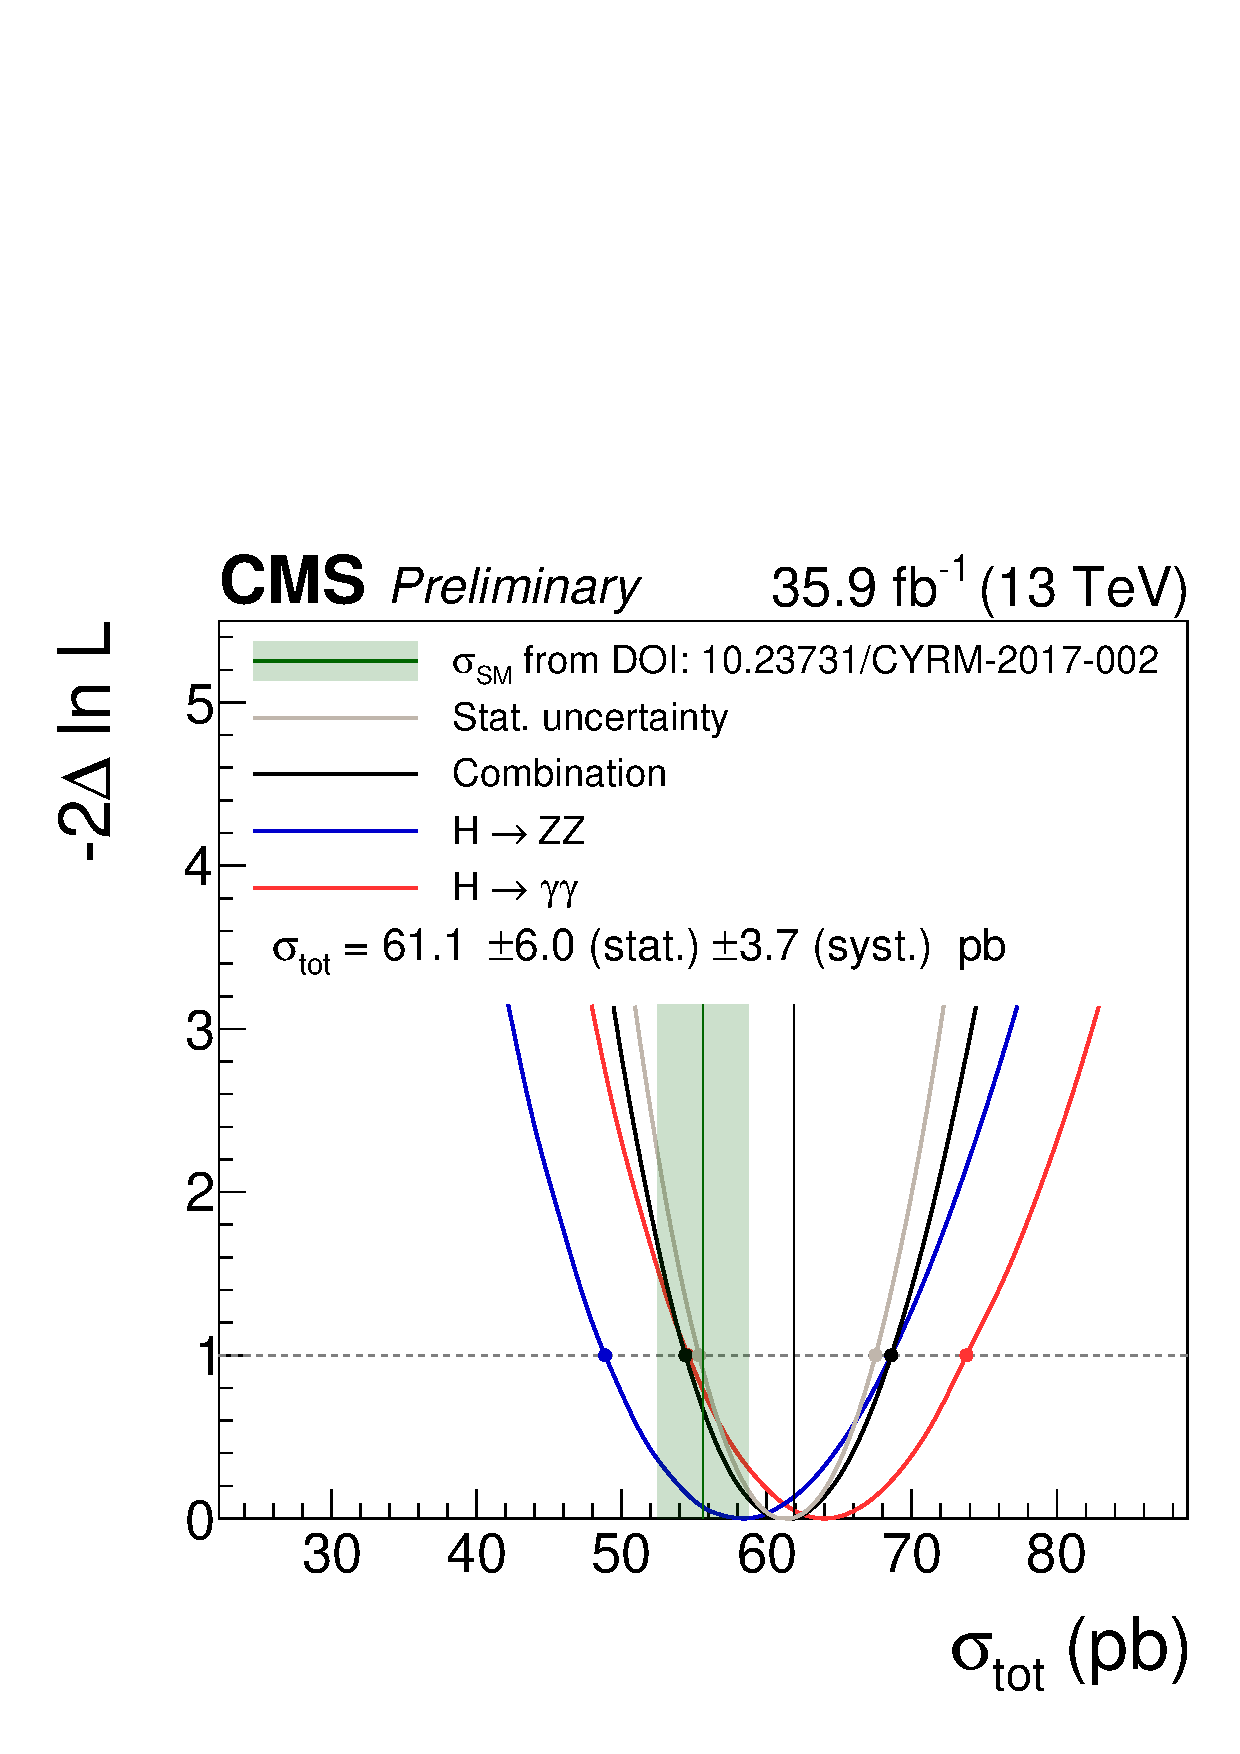
\includegraphics[width=\cmsFigWidth]{img/resultsapproval/reworked/scans_totalXS.pdf}
    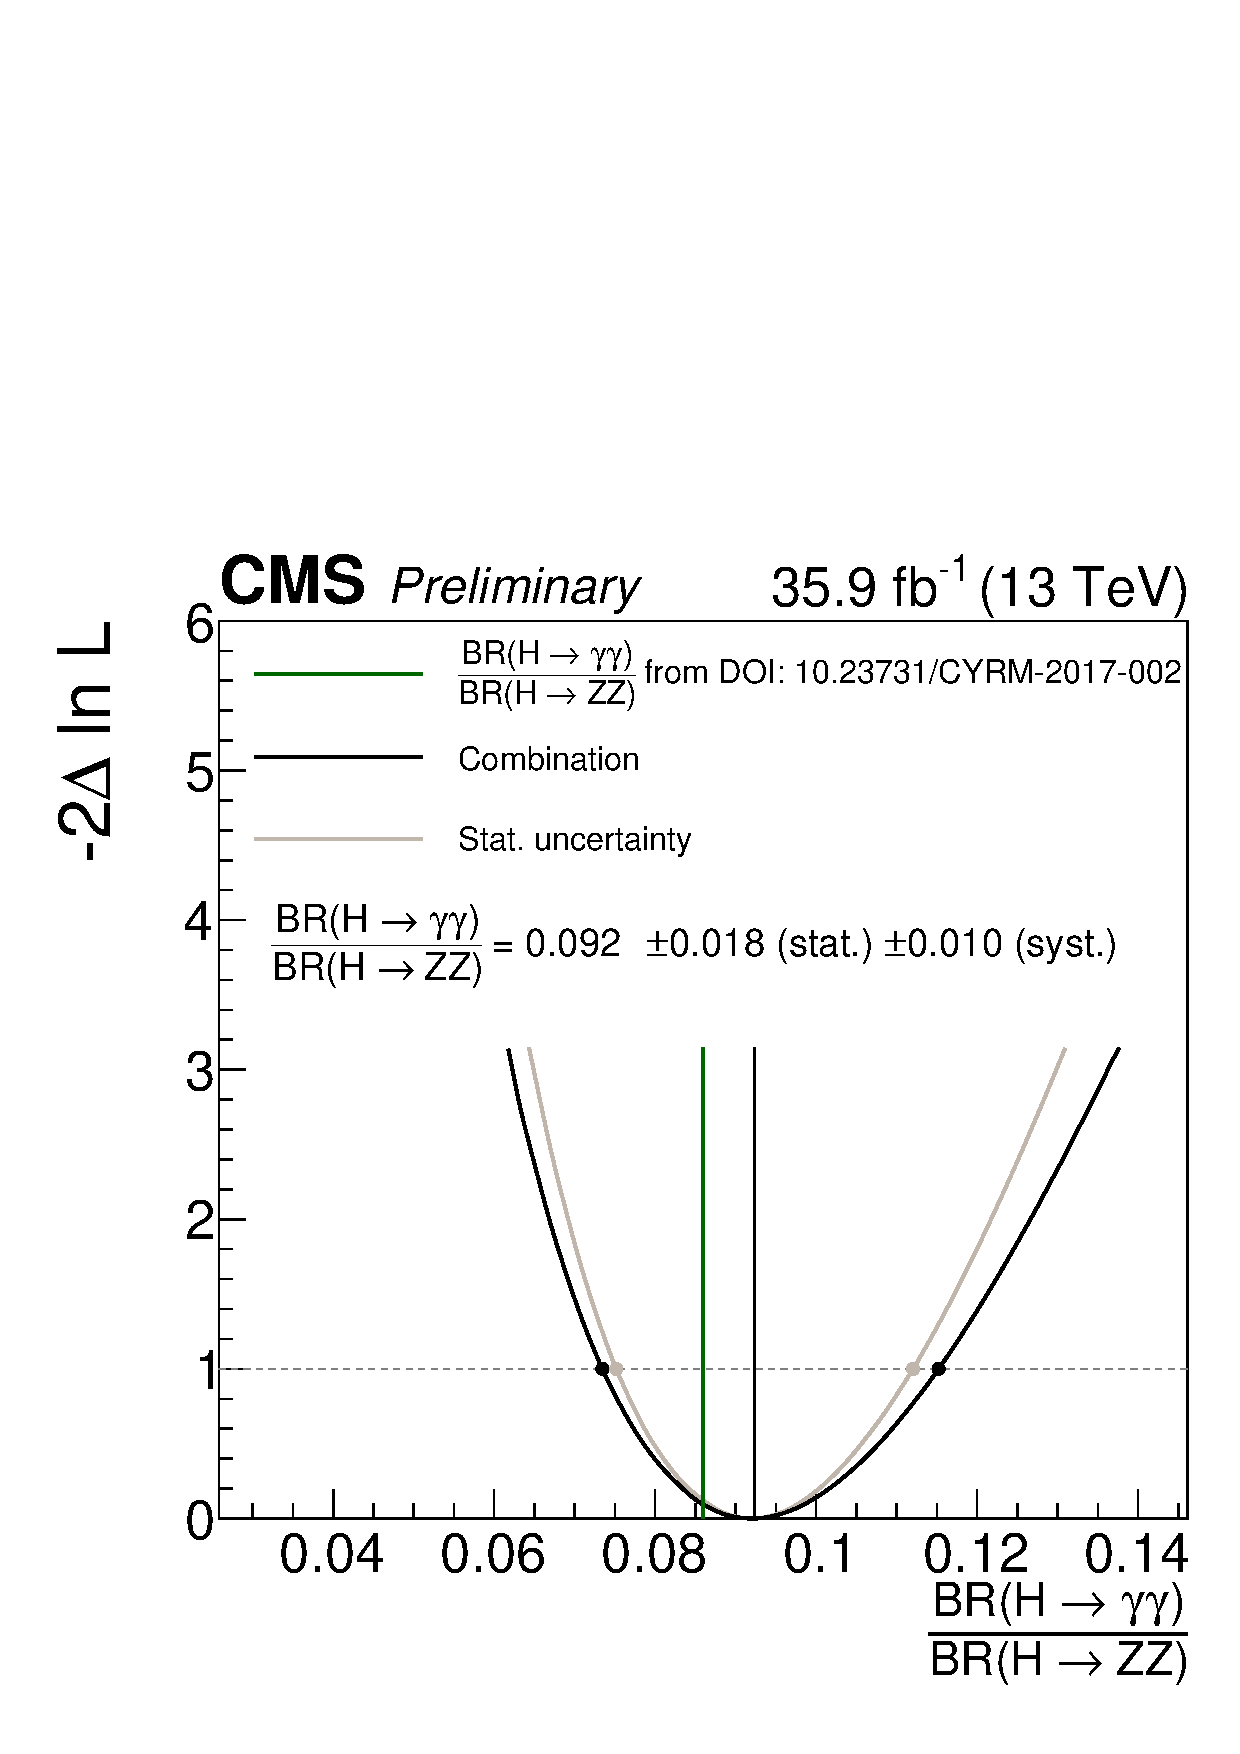
\includegraphics[width=\cmsFigWidth]{img/resultsapproval/reworked/scans_ratioOfBRs.pdf}
    \caption{
        (\cmsLeft) Scan of the total cross section $\sigma_\text{tot}$, based on a combination of the total cross sections from $\hgg$ ($64.0\pm9.6$\pb) and $\hzz$ ($58.2\pm9.8$\pb.
        % 
        (\cmsRight) Scan of the ratio of branching fractions $R$ based on a combination of $\hgg$ and $\hzz$, while profiling all other parameters.
        % 
        The filled markers indicate the one standard deviation interval.
        % 
        % \pasq{
        %     Remove `Preliminary', move legend to the right, move `CMS' to inside the plot. 
        %     }
        % \tk{Will do this later as someone is bound to have comments on this plot anyway.}
        }
    \label{fig:RatioOfbrsAndTotalXSscan}
  \end{center}
\end{figure}


% ____________________________________________________________________________
\subsection{Combinations of differential observables}
\label{sec:noncouplingresults}

The differential cross sections for the observables $\pth$, $\njets$, $\absy$ and $\ptjet$ are shown in
Fig~\ref{fig:CombinedSpectra_pth}, \ref{fig:CombinedSpectra_njets}, \ref{fig:CombinedSpectra_rapidity}, and \ref{fig:CombinedSpectra_ptjet}, including differential cross sections for Higgs production through gluon fusion for the observable $\pth$.
% 
Corresponding bin-to-bin correlation matrices are given in Appendix~\ref{sec:binToBinCorrelationMatrices}.
% 
For the observables $\pth$, $\njets$ and $\ptjet$, the last bin is an overflow bin; here the cross section is given in \pb, and is divided by the bin width of the second-to-last bin (ensuring that if the integrated cross sections in the last and second-to-last bin are equal, the value in the histogram is the same).
% 
Overall no significant deviations from the SM prediction are observed.
% 
For the $\pth$ spectrum, the uncertainties are strongly statistically dominated; in particular, the systematic uncertainty is about half the statistical uncertainty in the last bin, and much smaller in all other bins.
% 
The uncertainty in the combination per bin varies between 30\% and 40\%.
% 
Relative to the spectrum of $\hgg$ alone, the uncertainty decrease achieved by the combination is most notable in the lower $\pt$ region.
% 
% The overall uncertainties vary between 30\% and 40\%, and decrease with respect to the individual decay channels most notably in the lower $\pt$ region.
% % 
% Overall, the uncertainty of the combination with respect to only $\hgg$ is about 15\% smaller.
% 
The contribution of $\hbb$ to the overall precision of the combination is strongest in the last $\pth$ bin.

\begin{figure}[hbtp]
  \begin{center}
    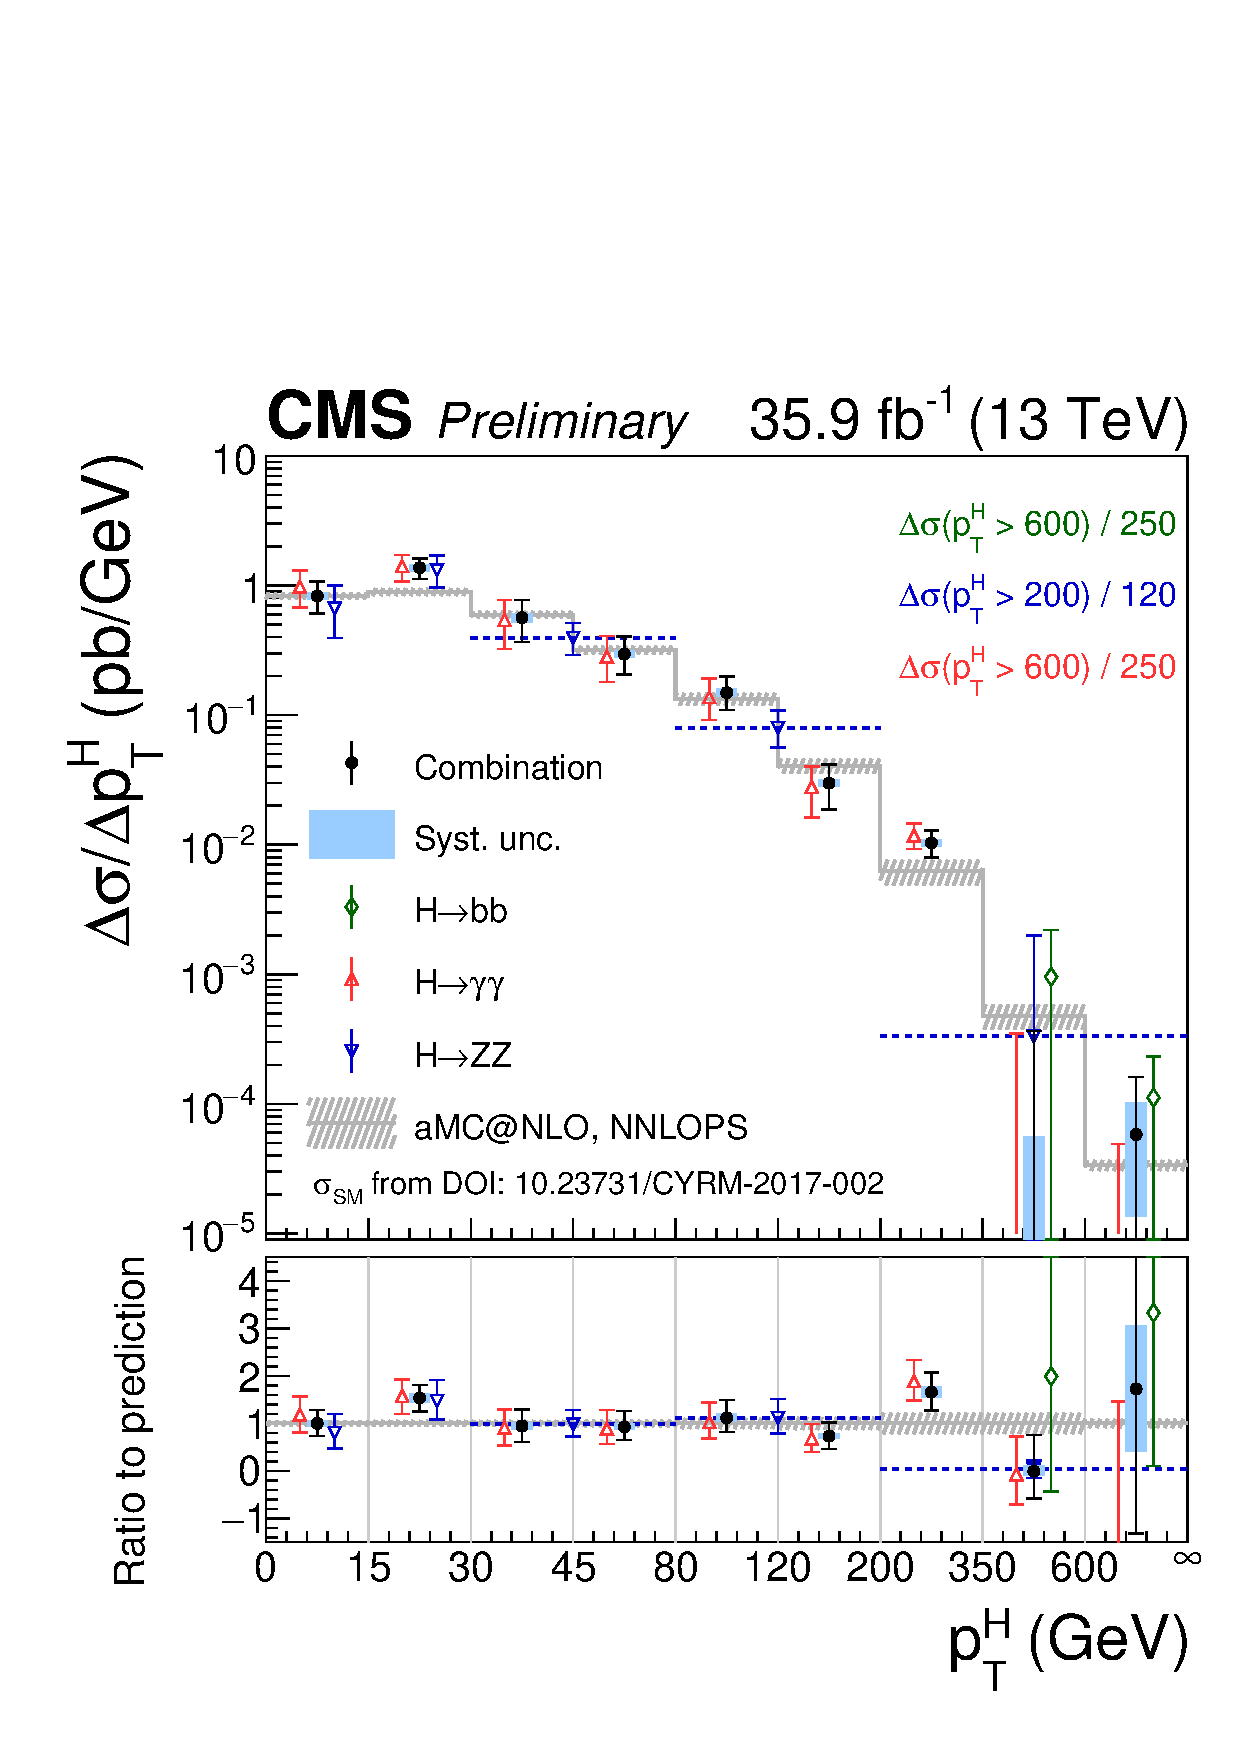
\includegraphics[width=\cmsFigWidth]{img/resultsapproval/reworked/spectra_pth_smH.pdf}
    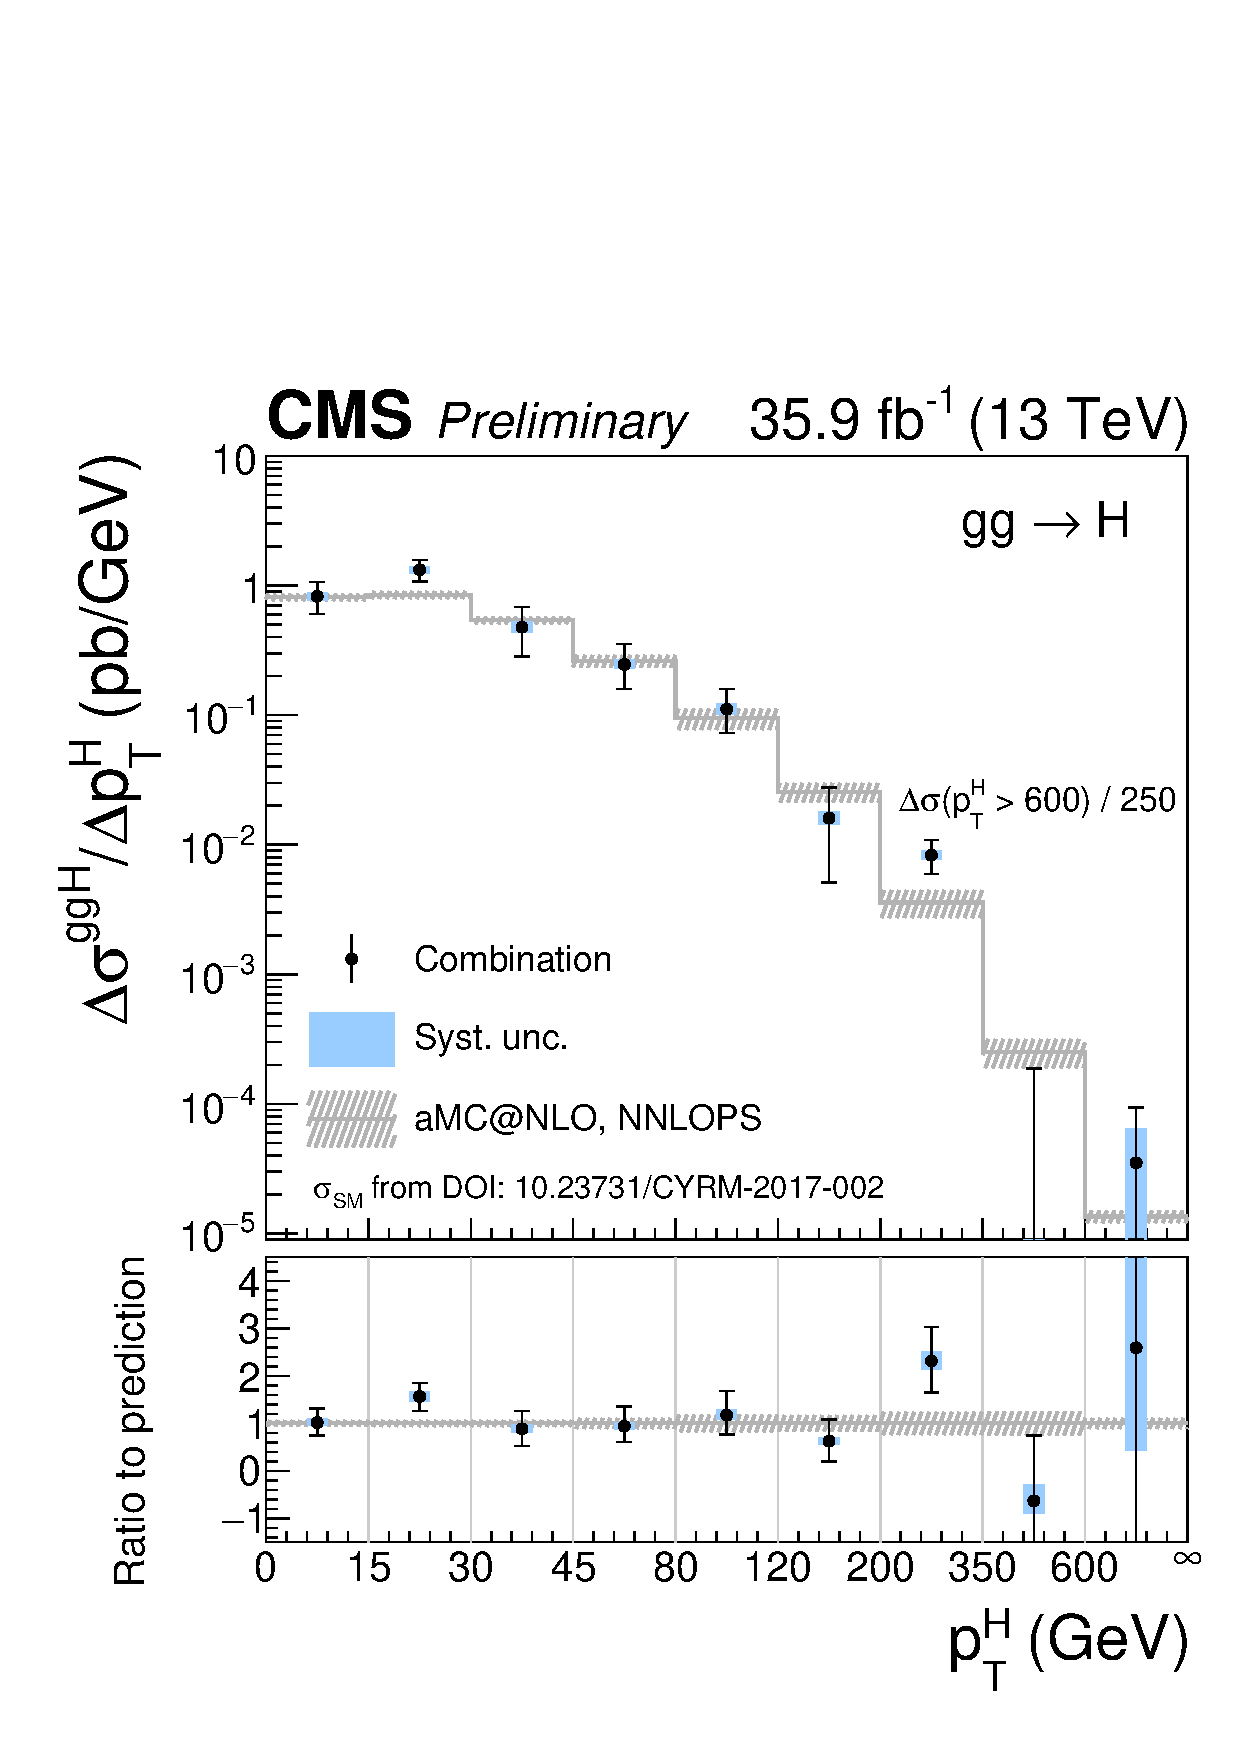
\includegraphics[width=\cmsFigWidth]{img/resultsapproval/reworked/spectra_pth_ggH.pdf}
    \caption{
        Best fit values and uncertainties of the cross sections and signal strengths.
        % 
        (\cmsLeft) $\pth$.
        (\cmsRight) $\pth$ while fixing non-gluon-fusion contributions to their SM expectation.
        % 
        % \pasq{Different markers per spectrum, integrals need to be bigger and different.
        % }
        % \tk{Will do this later as someone is bound to have comments on this plot anyway.}
        }
    \label{fig:CombinedSpectra_pth}
  \end{center}
\end{figure}

\begin{figure}[hbtp]
  \begin{center}
    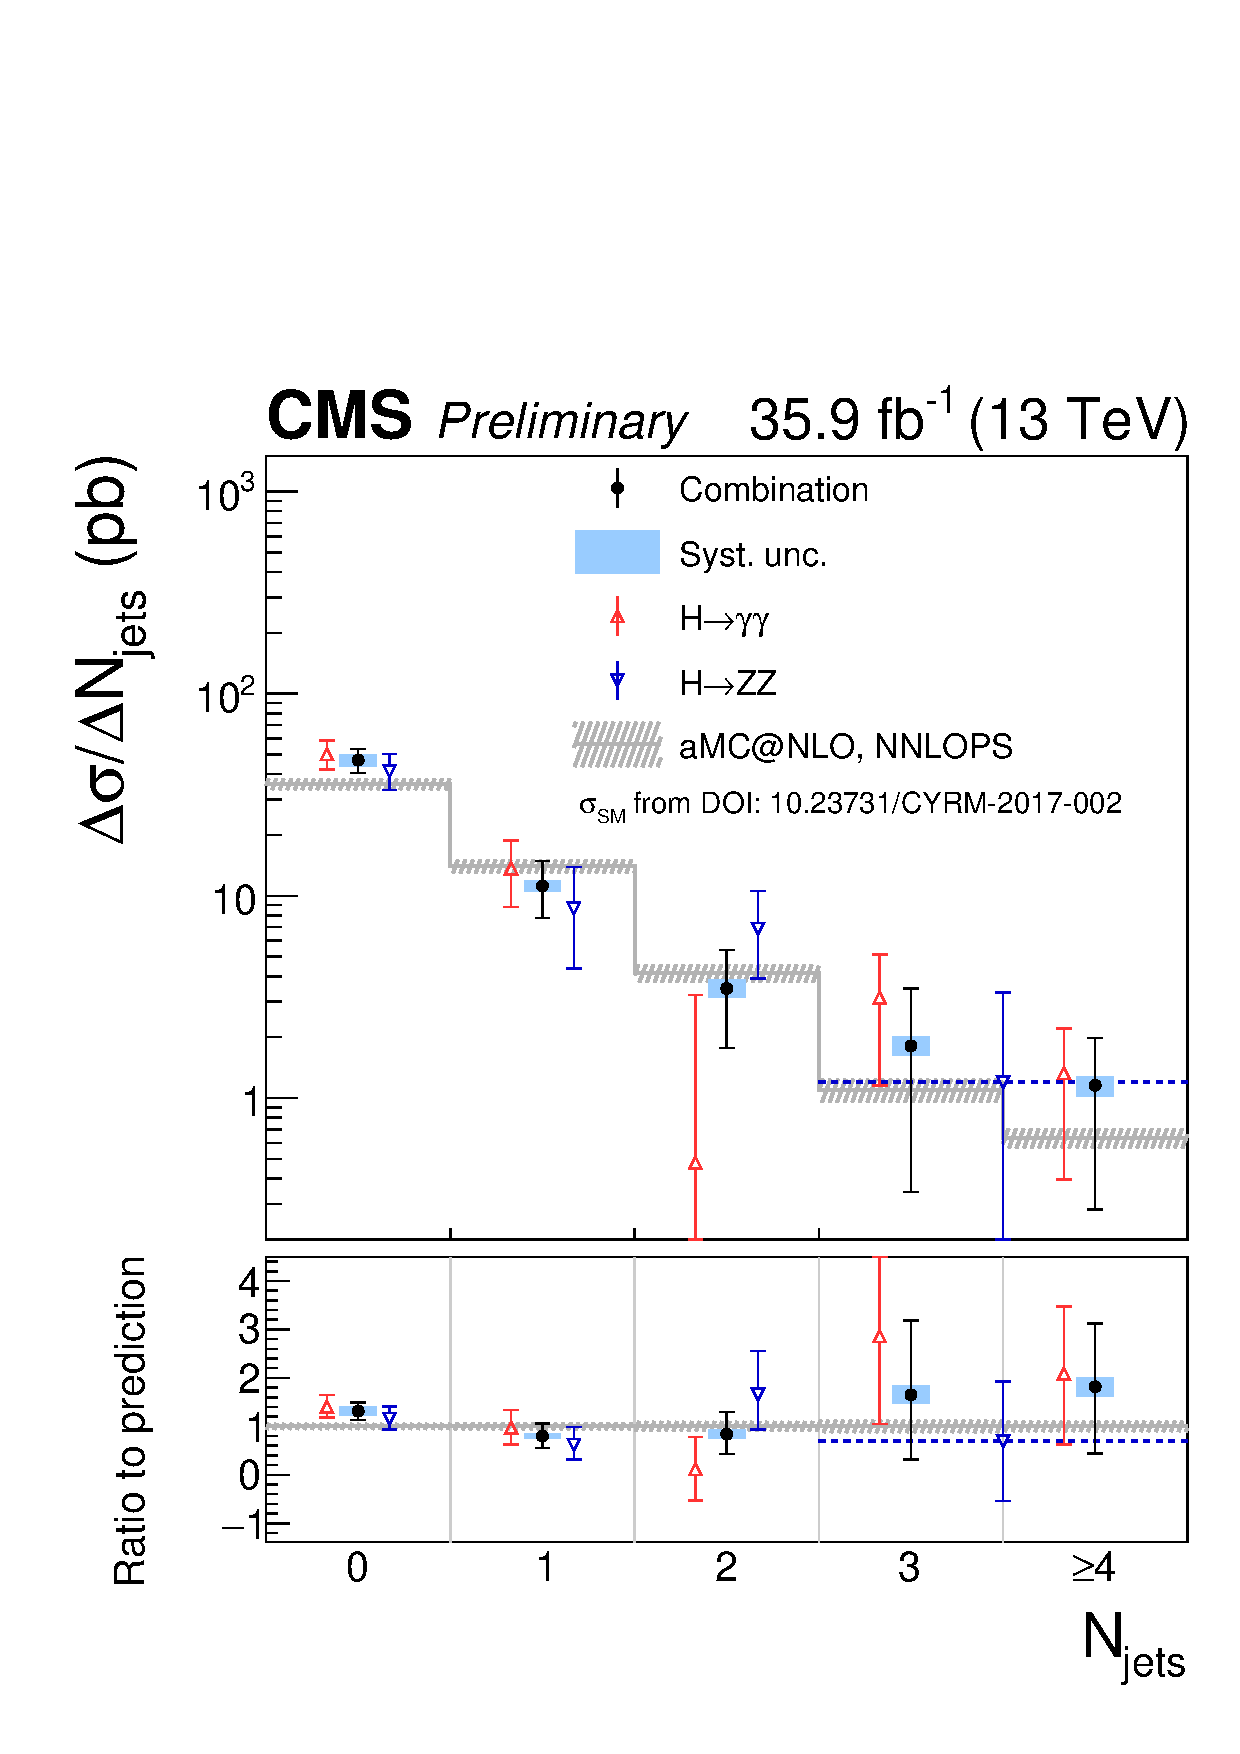
\includegraphics[width=\cmsFigWidth]{img/resultsapproval/reworked/spectra_njets.pdf}
    \caption{
        Best fit values and uncertainties of the cross sections and signal strengths for the $\njets$-spectrum.
        }
    \label{fig:CombinedSpectra_njets}
  \end{center}
\end{figure}

\begin{figure}[hbtp]
  \begin{center}
    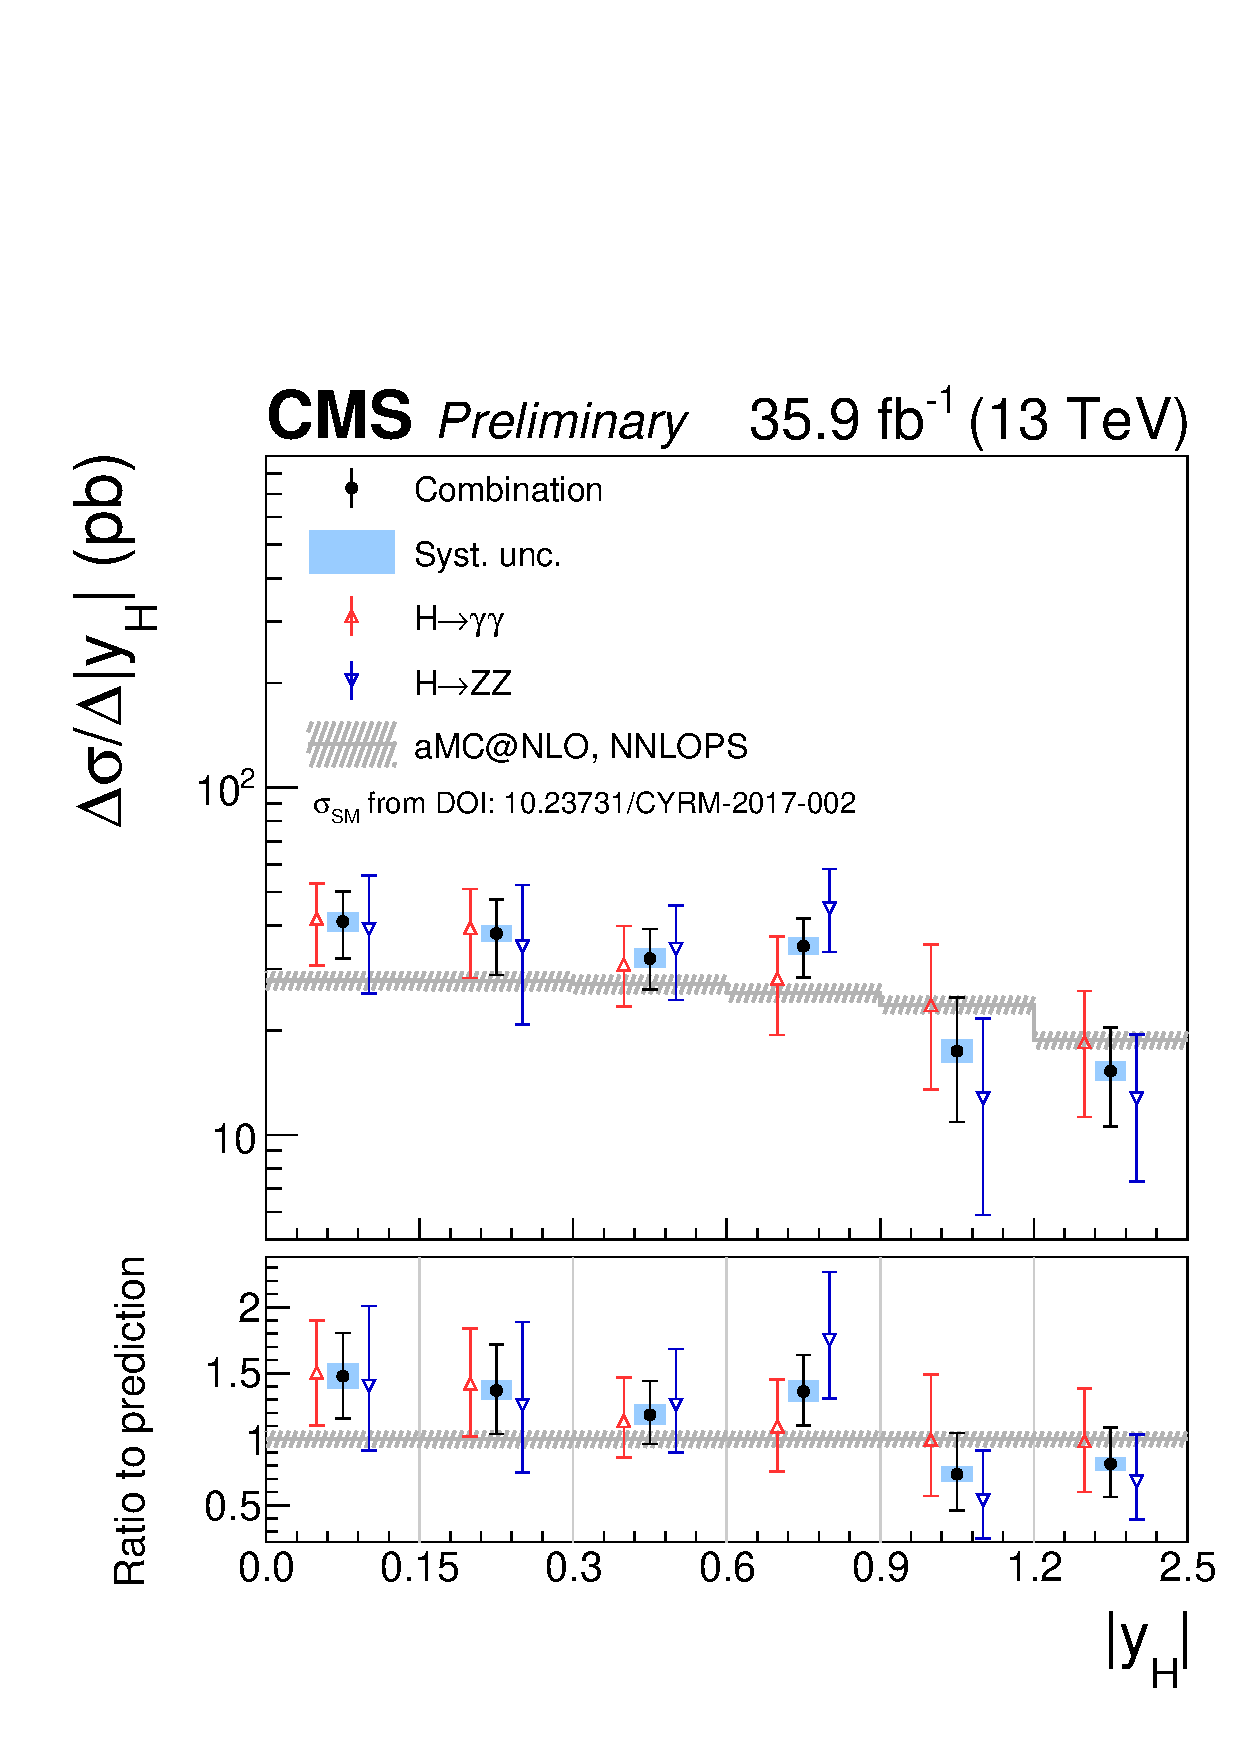
\includegraphics[width=\cmsFigWidth]{img/resultsapproval/reworked/spectra_rapidity.pdf}
    \caption{
        Expected best fit values and uncertainties of the cross sections and signal strengths for the $\absy$-spectrum.
        }
    \label{fig:CombinedSpectra_rapidity}
  \end{center}
\end{figure}

\begin{figure}[hbtp]
  \begin{center}
    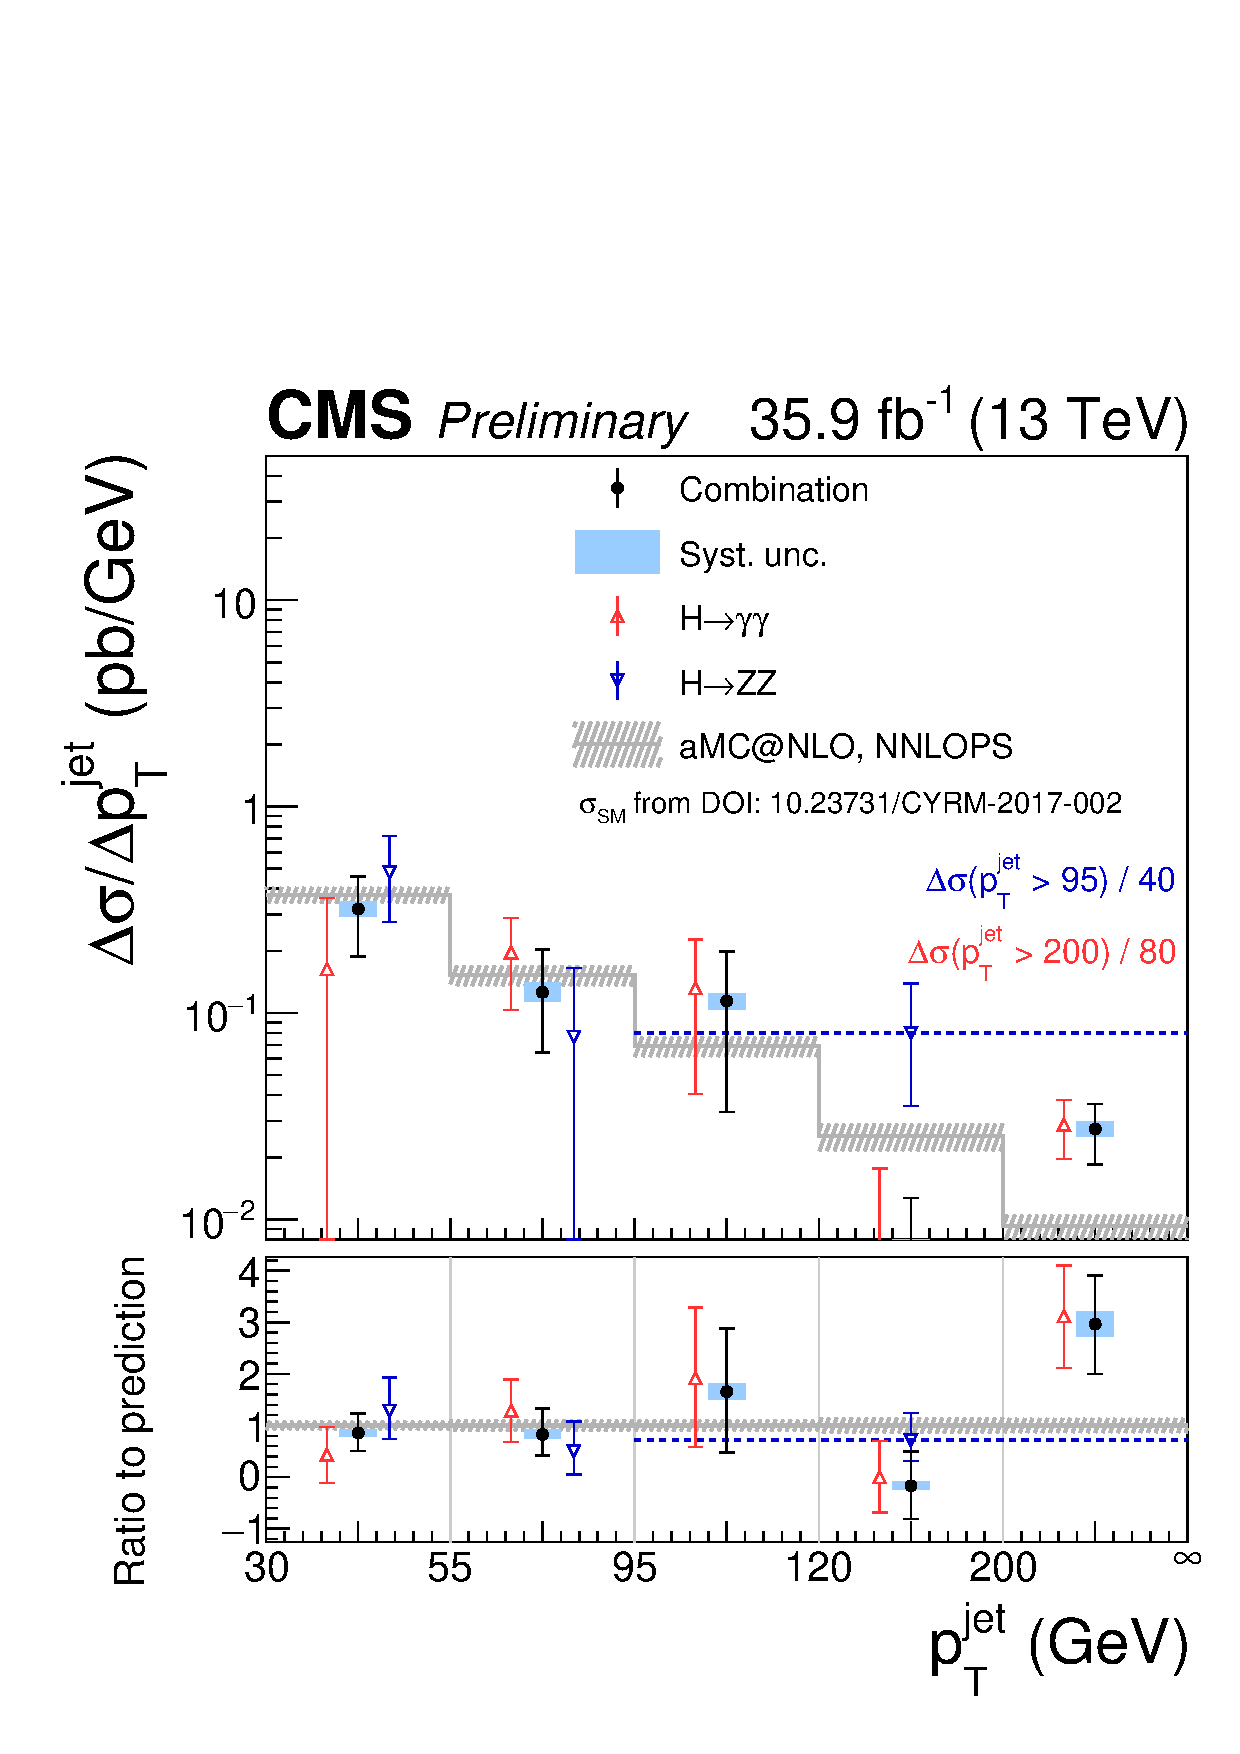
\includegraphics[width=\cmsFigWidth]{img/resultsapproval/reworked/spectra_ptjet.pdf}
    \caption{
        Expected best fit values and uncertainties of the cross sections and signal strengths for the $\ptjet$-spectrum.
        }
    \label{fig:CombinedSpectra_ptjet}
  \end{center}
\end{figure}


% ____________________________________________________________________________
\toggledclearpage
\subsection{Fits of Higgs coupling modifiers: \texorpdfstring{$\kappa_b$}{kb} vs. \texorpdfstring{$\kappa_c$}{kc}}
\label{sec:ResultsKappabKappac}

Figure~\ref{fig:scans_kappabkappac_nominal}(\cmsLeft) shows the one and two standard deviation contours of the fit of the $\kappa_b/\kappa_c$ parametrization from Ref.~\cite{Bishara:2016jga} to data.
% using the likelihood function described in Sec.~\ref{sec:statisticalanalysis}
% , including the contours obtained using only the $\hgg$ or $\hzz$ data.
% 
The calculations from Ref.~\cite{Bishara:2016jga} are given up to the scale of the Higgs mass, and thus $\hbb$ (whose $\pth$ spectrum starts at $\pth=350$\GeV) is not used as input for the results obtained here.
% 
% \arc{``which the parametrization for κb and κc is specified'' $\rightarrow$ you mean in the paper ? In addition you can say why it is not reliable theoretically, if the argument is given somewhere.}
% 
% Hence it is not included the $\kappa_b$ vs. $\kappa_c$ log-likelihood fit.
% 
The bin-to-bin correlations of the theoretical uncertainties are implemented as described in Sec.~\ref{sec:systematics}. 
% 
% 
The substructure on the combined scan shows a ring shape around the origin, and an almost one standard deviation agreement with the SM prediction.
% 
% 
% The substructure on the combined scan shows a ring shape around the origin, in which the origin and the SM expectation are not included, although these points are contained in the region allowed at $2\sigma$.
% 
% A comparable proof-of-concept study was already performed in Ref.~\cite{Bishara:2016jga} using ATLAS data from Run I, yielding the overall bounds $\kappa_c \in [ -16, 18 ]$.~\tk{Edit here posssibly.}

% img/resultsapproval/reworked/multicont_Yukawa_couplingdependentBRs.pdf
% img/resultsapproval/reworked/multicont_Yukawa_floatingBRs.pdf


In order to evaluate the effect of the shape on the constraints on $\kappa_b$ and $\kappa_c$, the procedure is repeated with freely floating branching fractions, effectively removing constraints from the total width and from the overall normalization.
% 
The result of this fit is shown in Fig.~\ref{fig:scans_kappabkappac_nominal}(\cmsLeft).
% 
As expected, the range of allowed values of $\kappa_b$ and $\kappa_c$ is much wider than in the case of coupling-dependent branching fractions.


\begin{figure}[hbtp]
  \begin{center}
    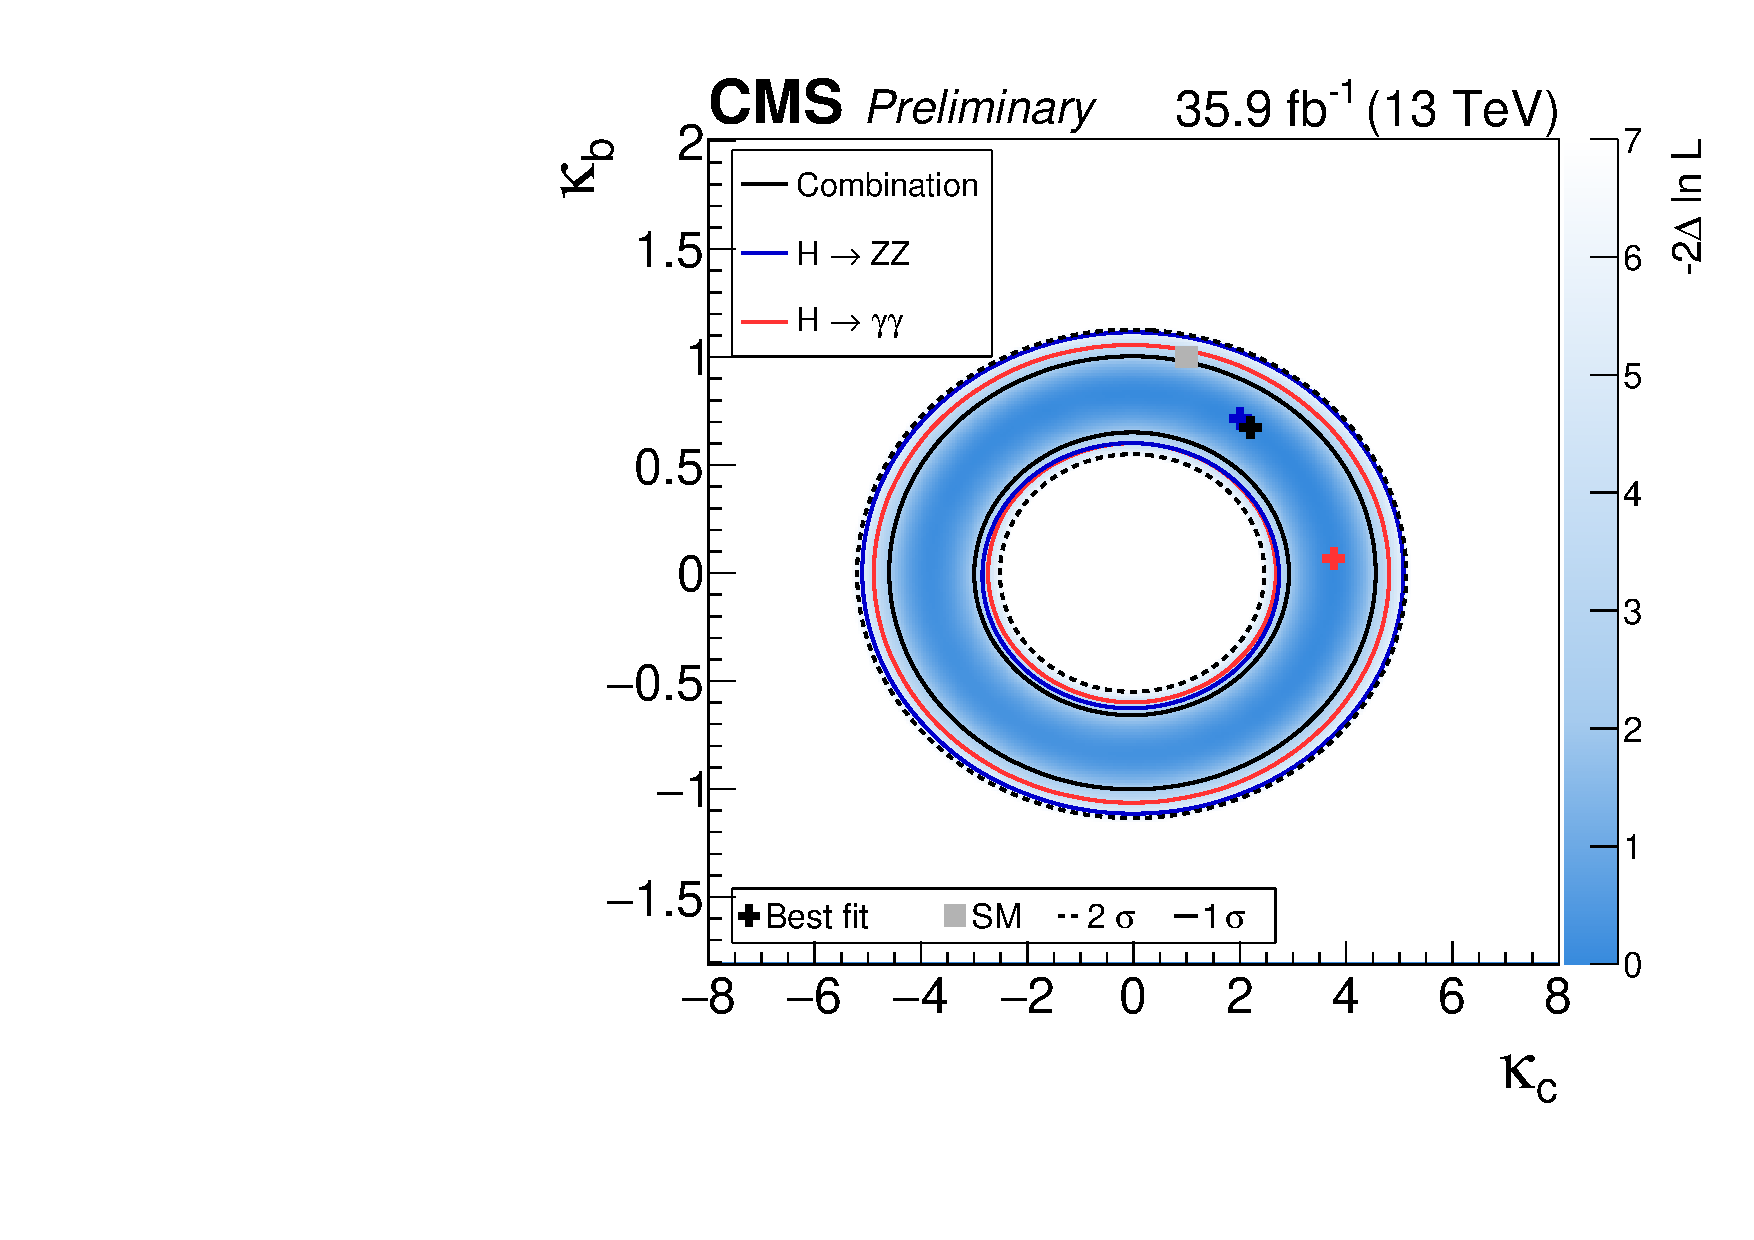
\includegraphics[width=0.49\linewidth]{img/resultsapproval/reworked/multicont_Yukawa_couplingdependentBRs.pdf}
    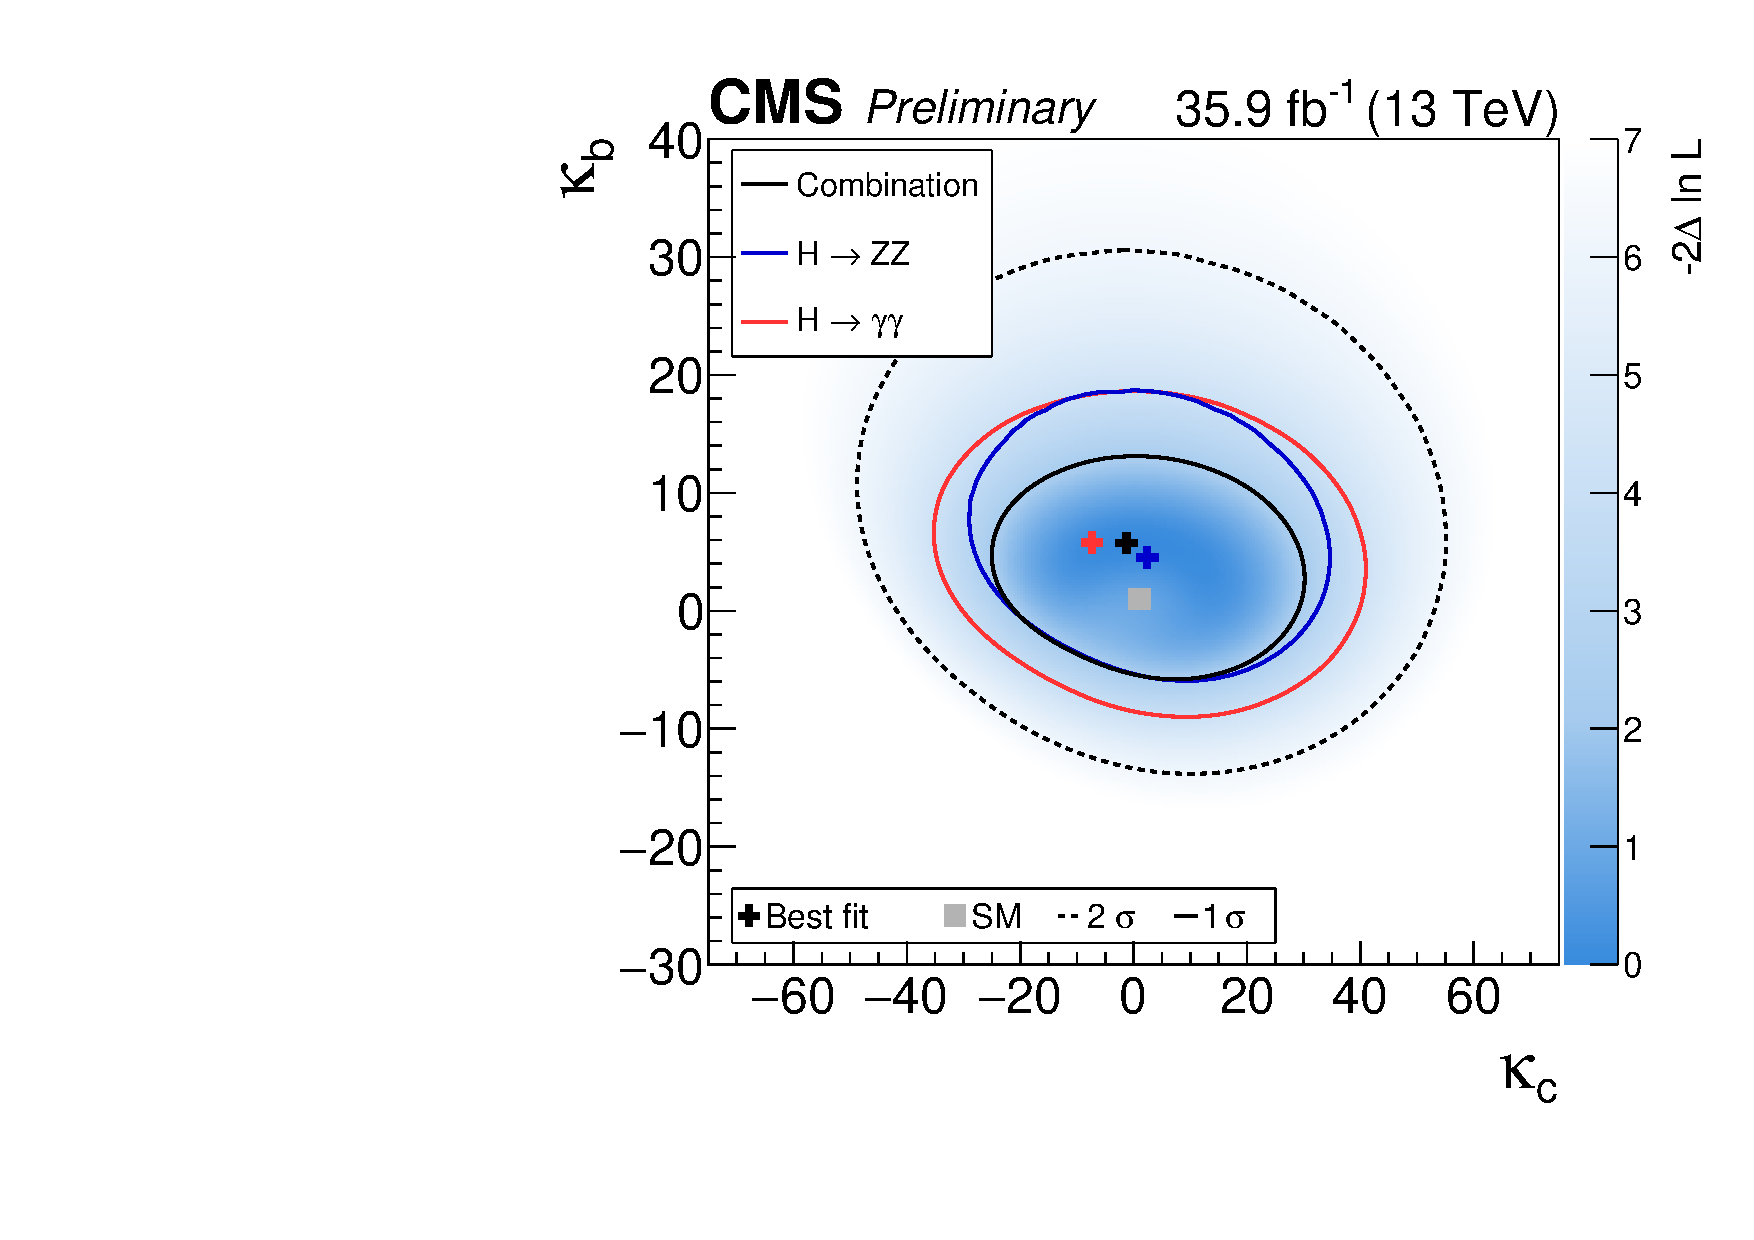
\includegraphics[width=0.49\linewidth]{img/resultsapproval/reworked/multicont_Yukawa_floatingBRs.pdf}
    % 
    \caption{
        Simultaneous fit results for $\kappa_b$ and $\kappa_c$.
        % 
        (\cmsLeft) One and two standard deviation contours are shown for the combined ($\hgg$ and $\hzz$) fit to data and for $\hgg$ and $\hzz$ separately, assuming a coupling dependency of the branching fractions.
        % 
        (\cmsRight) One and two standard deviation contours are shown for the combined ($\hgg$ and $\hzz$) fit to data and for $\hgg$ and $\hzz$ separately, assuming freely floating branching fractions.
        % 
        % 
        % Simultaneous fit results for $\kappa_b$ and $\kappa_c$, showing one- and two-$\sigma$ contours for the fit to data.
        % % 
        % % including fit results using only the $\hgg$ and $\hzz$ inputs.
        % % 
        % (\cmsLeft) Branching fractions scaling with $\kappa_b$ and $\kappa_c$.
        % % 
        % (\cmsRight) Branching fractions freely floating, effectively yielding the constraint obtained solely from the shape.
        }
    \label{fig:scans_kappabkappac_nominal}
  \end{center}
\end{figure}


Separate limits can be set on $\kappa_b$ and $\kappa_c$ by profiling one coupling and scanning over the other.
% 
% Limits on $\kappa_b$ and $\kappa_c$ individually can be set by profiling one coupling and scanning over the other.
% 
The results of these single-coupling scans are shown in Fig.~\ref{fig:scans_kappabkappac_oneDimScans} and Fig.~\ref{fig:scans_kappabkappac_oneDimScans_scenario2}.
% 
The observed uncertainties in the one-dimensional scans are:
% 
% \clearpage
\begin{equation}
\label{eq:kappasensitivity}
\begin{array}{c}
\kappabLeftObserved < \kappa_b < \kappabRightObserved  \quad(\kappabLeftAsimov < \kappa_b < \kappabRightAsimov \;\; \text{expected})  \,,
\\[8pt]
\kappacLeftObserved < \kappa_c < \kappacRightObserved \quad(\kappacLeftAsimov < \kappa_c < \kappacRightAsimov \;\; \text{expected})
\,,
\end{array}
\end{equation}
% 
in the case of branching fractions that depend on $\kappa_b$ and $\kappa_c$, and
% 
\begin{equation}
\label{eq:kappasensitivity}
\begin{array}{c}
\kappabLeftObservedFLOATINGBRS < \kappa_b < \kappabRightObservedFLOATINGBRS  \quad(\kappabLeftAsimovFLOATINGBRS < \kappa_b < \kappabRightAsimovFLOATINGBRS \;\; \text{expected})  \,,
\\[8pt]
\kappacLeftObservedFLOATINGBRS < \kappa_c < \kappacRightObservedFLOATINGBRS \quad(\kappacLeftAsimovFLOATINGBRS < \kappa_c < \kappacRightAsimovFLOATINGBRS \;\; \text{expected})
\,,
\end{array}
\end{equation}
% 
in the case of freely floated branching fractions.
% 
For the coupling-dependent branching fractions, the results are shaped predominantly by constraints from the total width rather than by distortions of the $\pth$ spectrum.
% 
If the branching fractions are fixed to their SM expectations, the one-dimensional scans yield the following expected uncertainties:
% 
\begin{equation}
\label{eq:kappasensitivity_fixedSMBRs}
\begin{array}{c}
-1.9 < \kappa_b < 2.9 \;\; (\text{expected})  \,,
 \\[8pt]
-8.7 < \kappa_c < 10.6 \;\; (\text{expected})
\,.
\end{array}
\end{equation}
% 
These limits are comparable to those in Ref.~\cite{Bishara:2016jga}, where $\kappa_c \in [ -16, 18 ]$, noting that the results here are based on a larger data set.
% 
The limits obtained are competitive with the limits from other direct search channels summarized in Sec.~\ref{sec:introduction}.


\begin{figure}[Hbtp]
  \begin{center}
    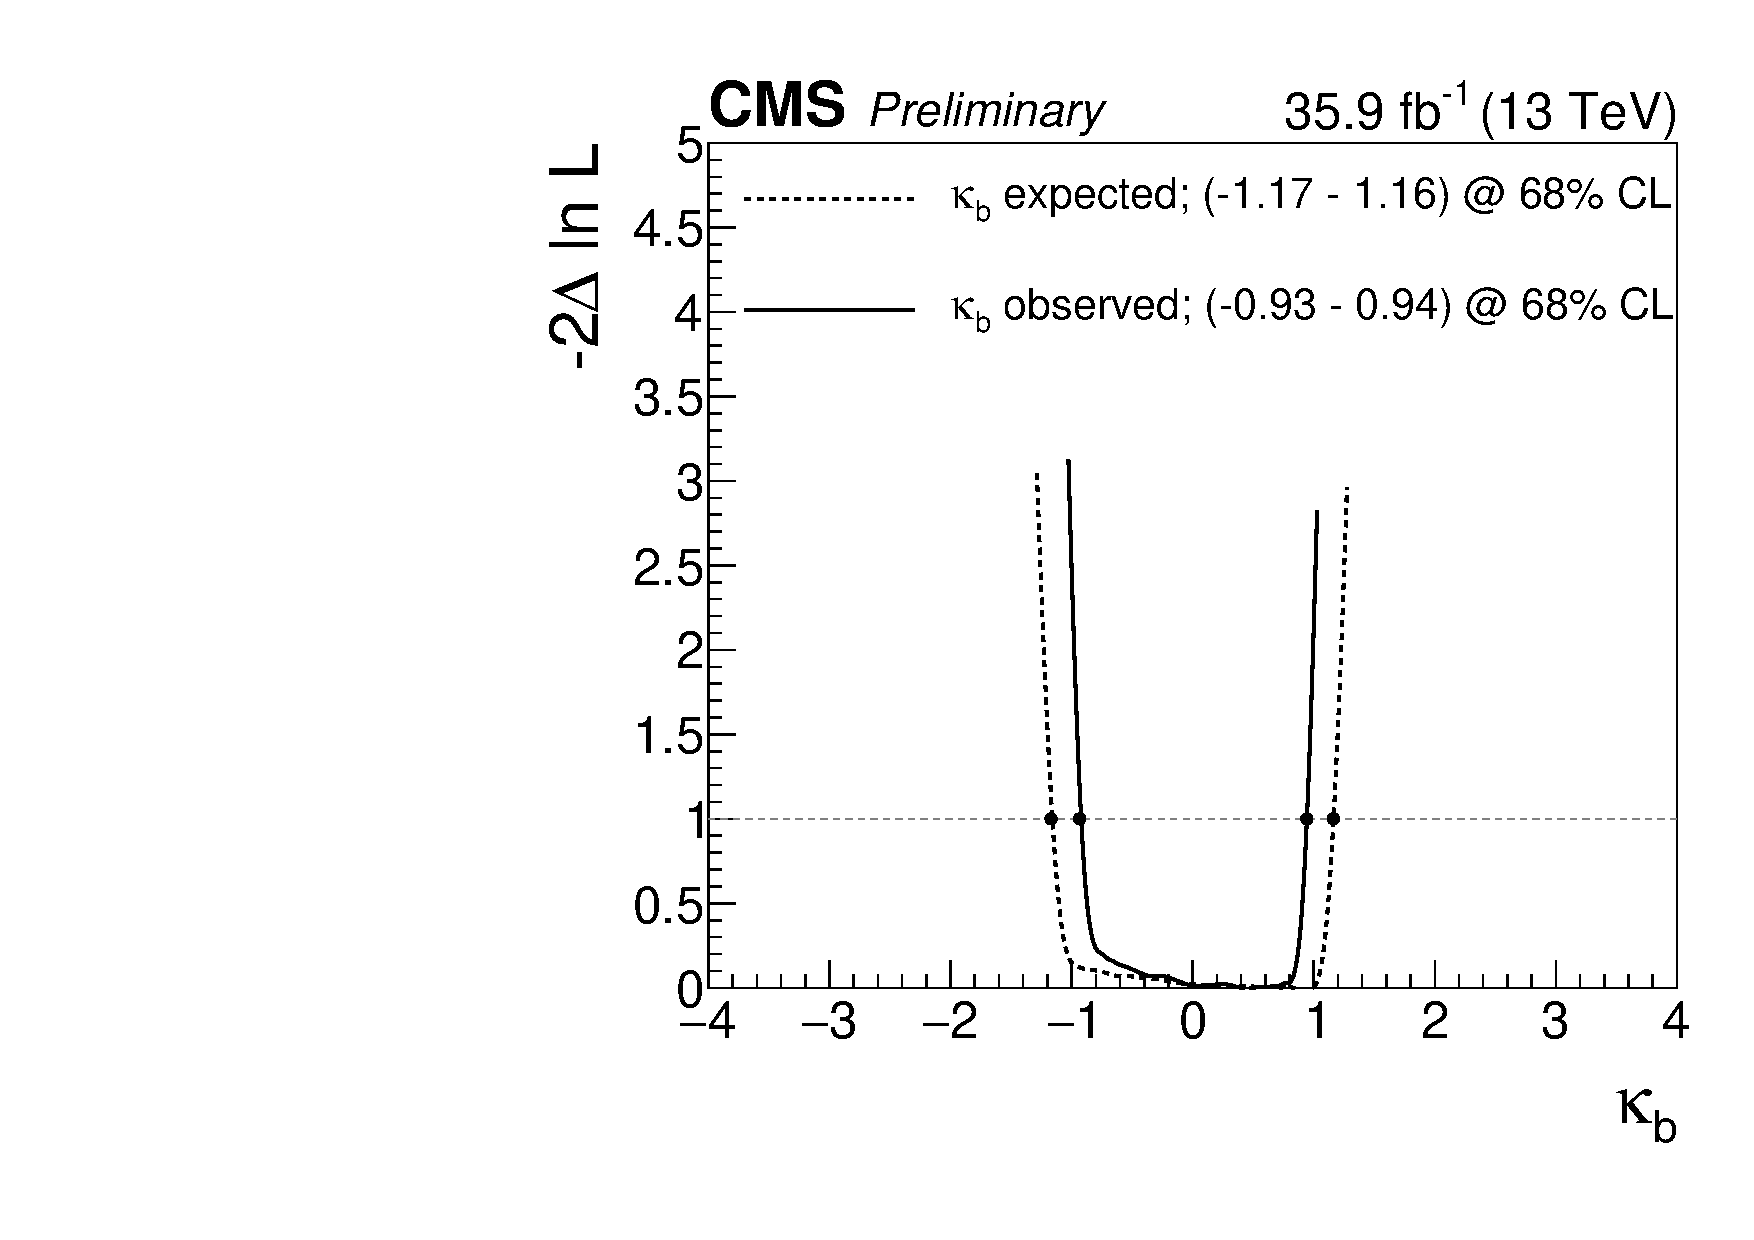
\includegraphics[width=\cmsFigWidth]{img/resultsapproval/reworked/onekappascan_kbkc_couplingdependentBRs_kappab.pdf}
    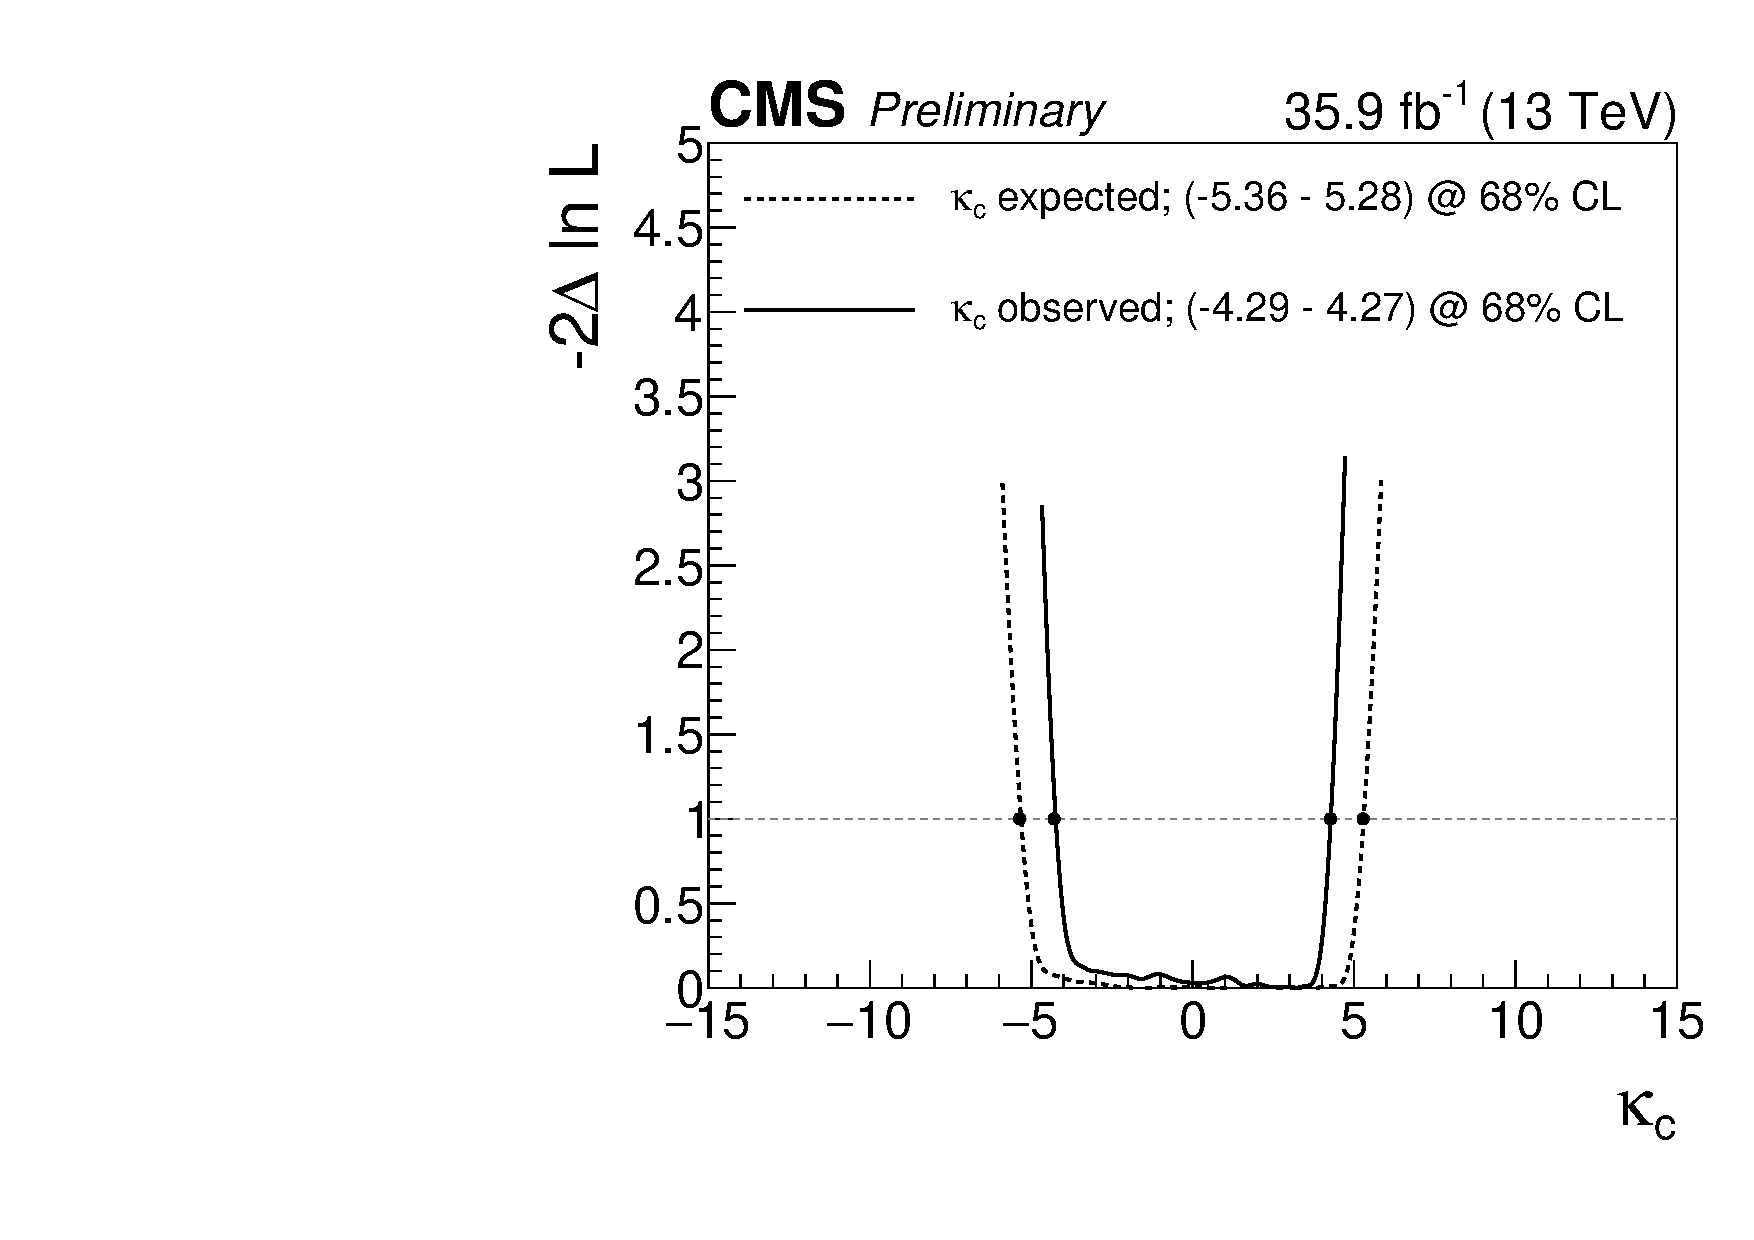
\includegraphics[width=\cmsFigWidth]{img/resultsapproval/reworked/onekappascan_kbkc_couplingdependentBRs_kappac.pdf}
    \caption{
        Scans of only one coupling, while profiling the other.
        % 
        The filled markers indicate the one standard deviation interval.
        % 
        The branching fractions were considered dependent on the values of the couplings.
        % 
        (\cmsLeft)
            Scan of $\kappa_b$ while profiling $\kappa_c$.
        (\cmsRight)
            Scan of $\kappa_c$ while profiling $\kappa_b$.
        }
    \label{fig:scans_kappabkappac_oneDimScans}
  \end{center}
\end{figure}

\begin{figure}[Hbtp]
  \begin{center}
    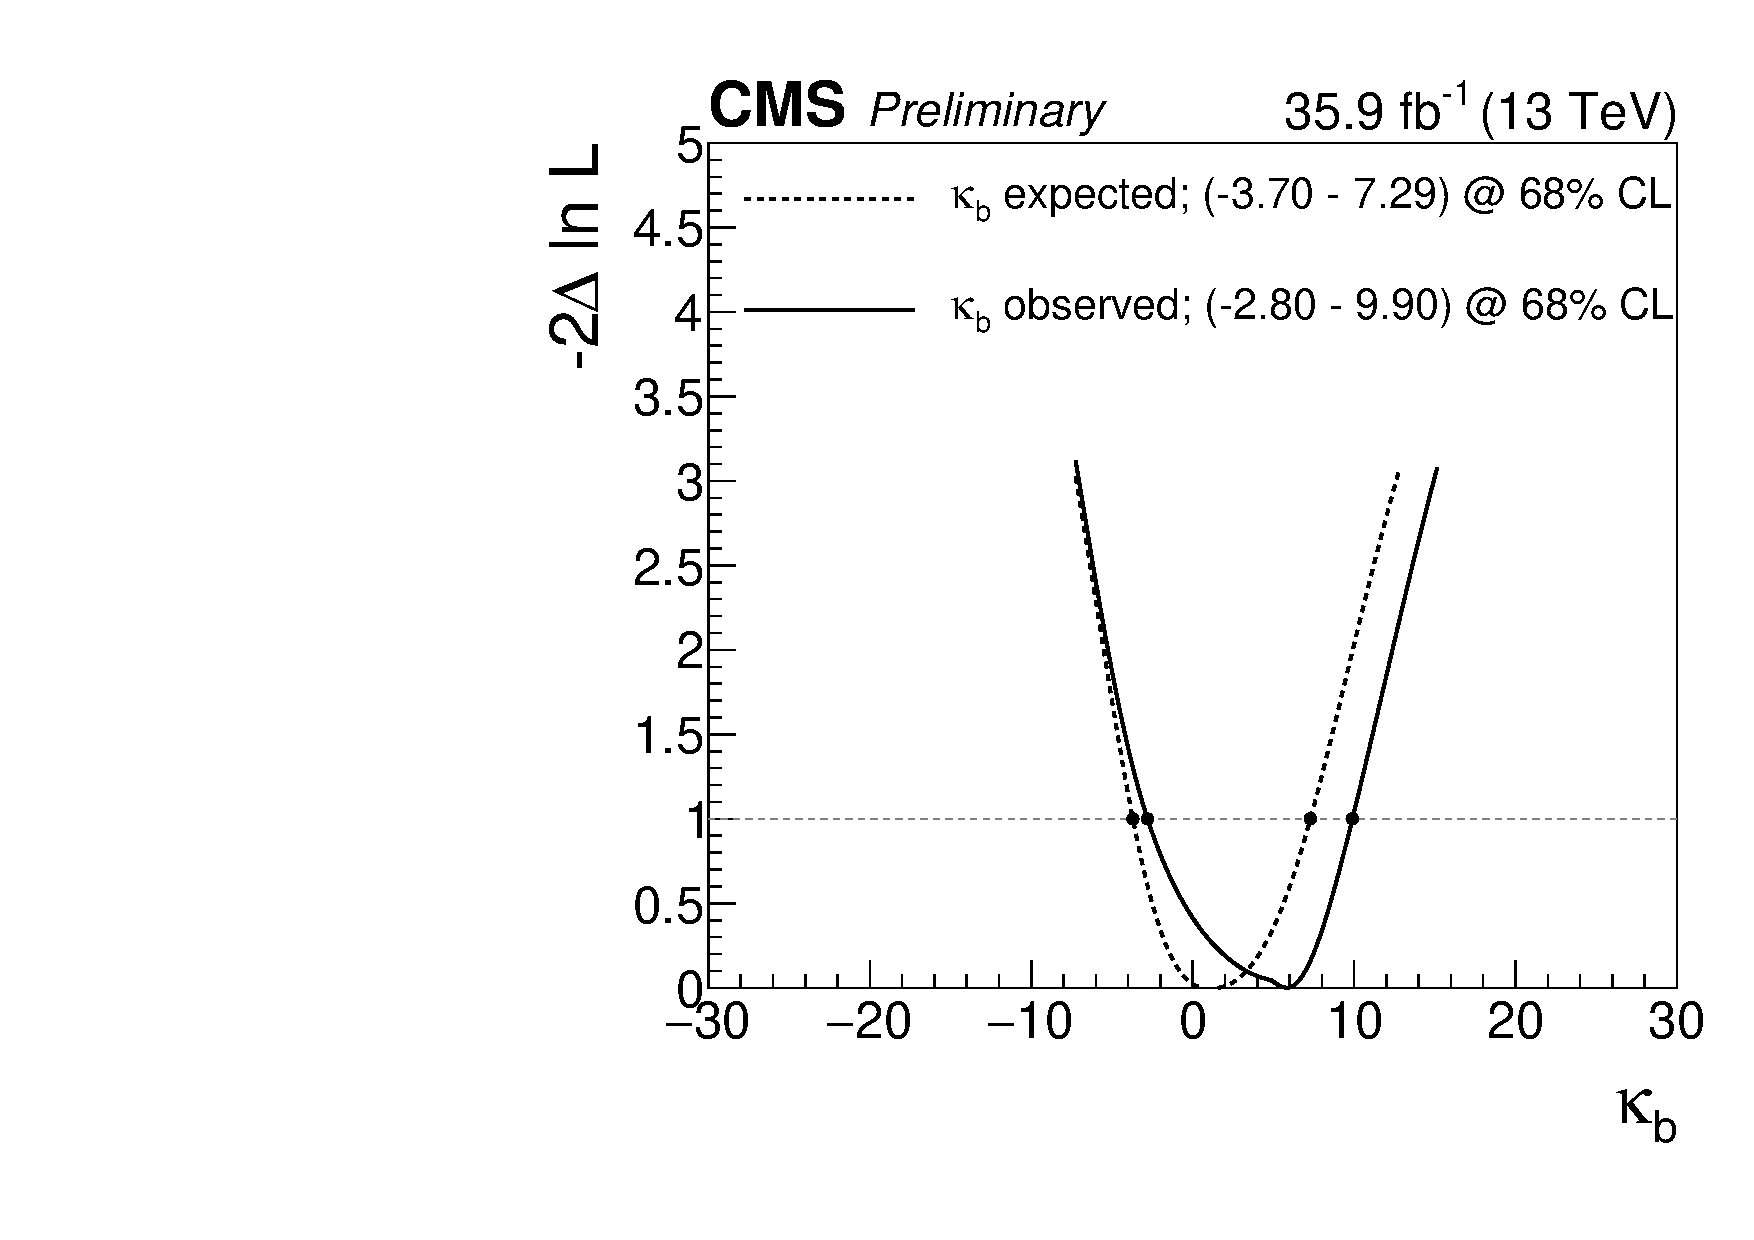
\includegraphics[width=\cmsFigWidth]{img/resultsapproval/reworked/onekappascan_kbkc_floatingBRs_kappab.pdf}
    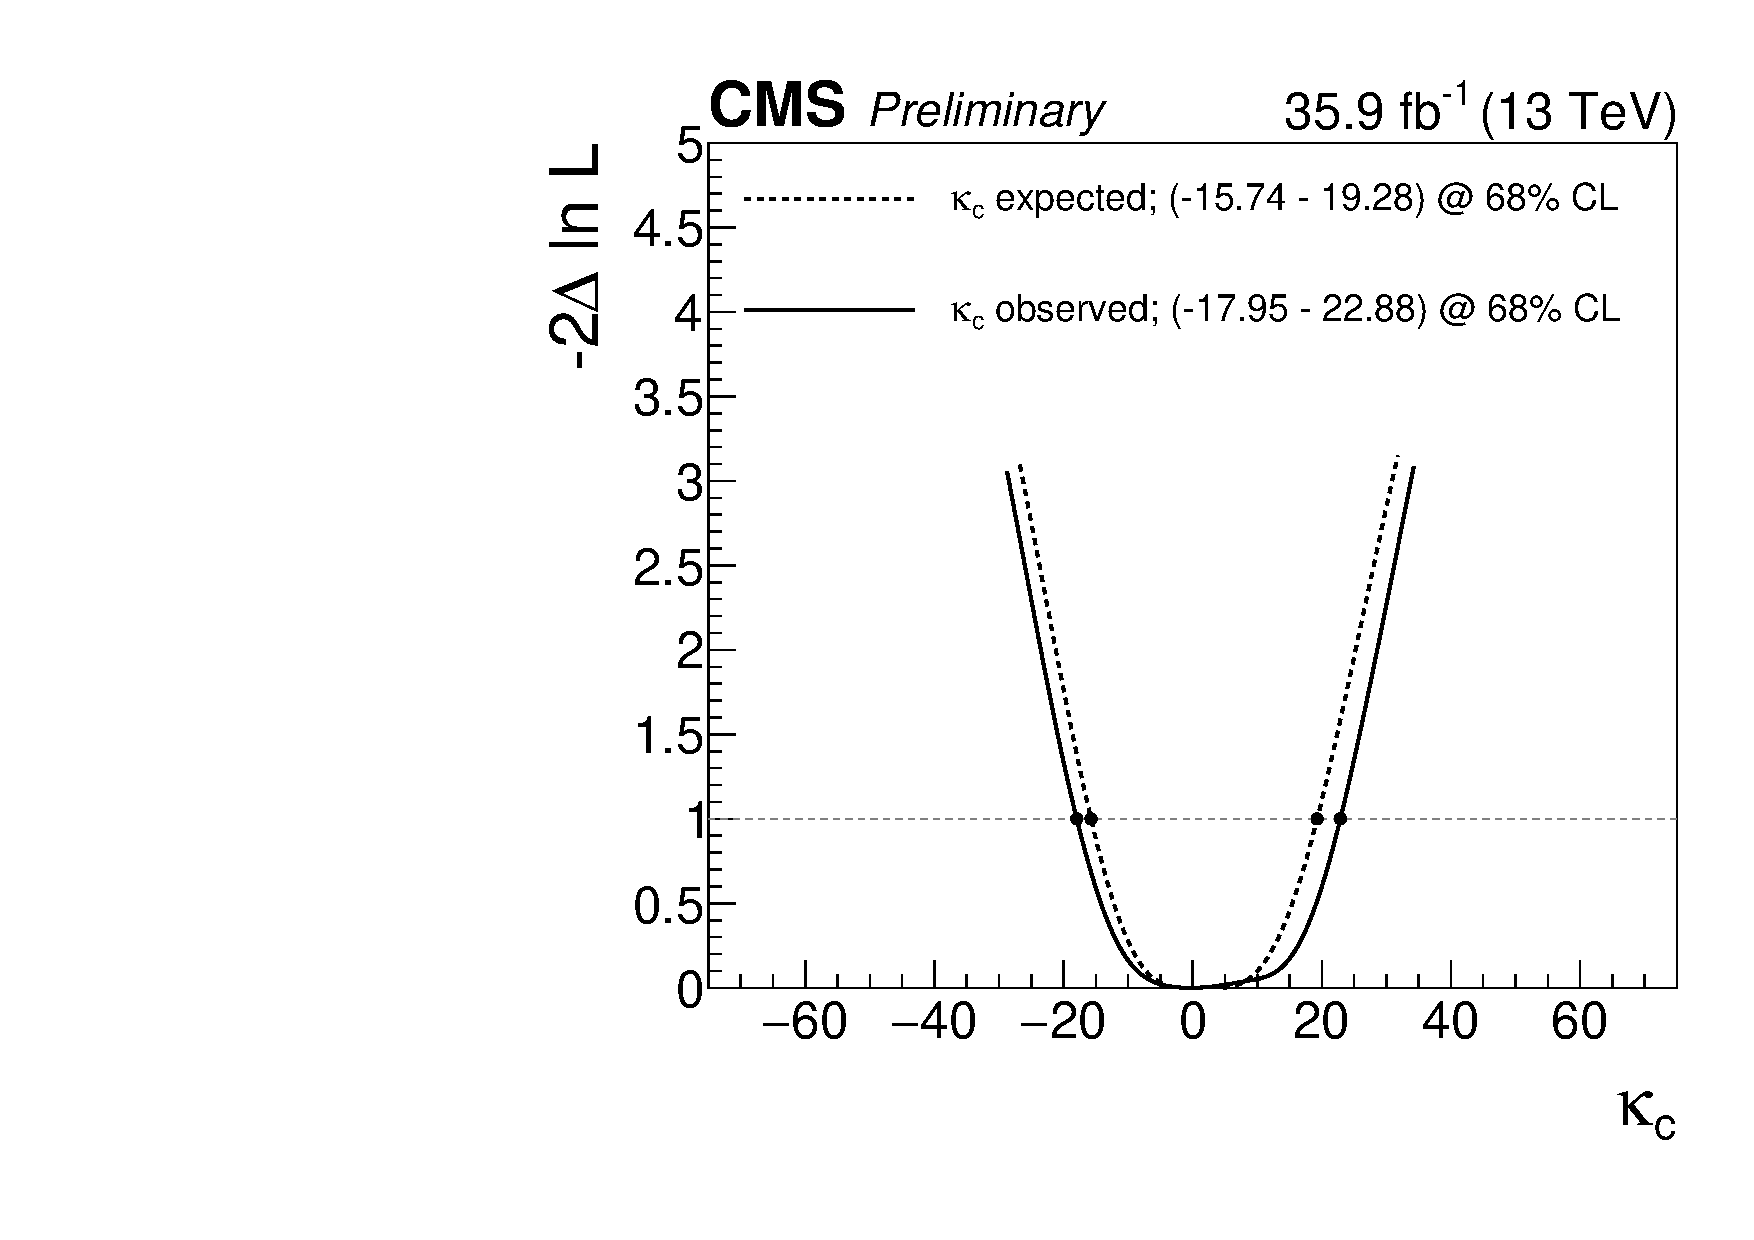
\includegraphics[width=\cmsFigWidth]{img/resultsapproval/reworked/onekappascan_kbkc_floatingBRs_kappac.pdf}
    \caption{
        Scans of only one coupling, while profiling the other.
        % 
        The filled markers indicate the one standard deviation interval.
        % 
        The branching fractions were freely floated in the fit.
        % 
        (\cmsLeft)
            Scan of $\kappa_b$ while profiling $\kappa_c$.
        (\cmsRight)
            Scan of $\kappa_c$ while profiling $\kappa_b$.
        }
    \label{fig:scans_kappabkappac_oneDimScans_scenario2}
  \end{center}
\end{figure}

% \clearpage
% \begin{equation}
%     s_i(\kappa_b, \kappa_c) =
%         \frac
%             {\sigma_i(\kappa_b, \kappa_c)}
%             {\sum_j \sigma_j(\kappa_b, \kappa_c)}
% \end{equation}







% ____________________________________________________________________________
\toggledclearpage
\subsection{Fits of Higgs coupling modifiers: \texorpdfstring{$\kappa_t$}{kt} vs. \texorpdfstring{$\cg$}{cg} and \texorpdfstring{$\kappa_t$}{kt} vs. \texorpdfstring{$\kappa_b$}{kb}}

% \begin{equation}
% \begin{align}
% % 
% s_i(\kappa_t, \cg)
%     &=
%     \frac
%         {\sigma_i(\kappa_t, \cg)}
%         {\sum_j \sigma_j(\kappa_t, \cg)}
%     \\
%     &=
%     \frac{
%         \sigma^\text{ggH}_i(\kappa_t, \cg) + \sigma^\text{xH}_i(\kappa_t, \cg)
%         }{
%         \sum_j \sigma^\text{ggH}_j(\kappa_t, \cg) + \sum_j \sigma^\text{xH}_j(\kappa_t, \cg)
%         }
%     \\
%     &=
%     \frac{
%         \sigma^\text{ggH}_i(\kappa_t, \cg) + \sigma^\text{xH}_i(\kappa_t, \cg)
%         }{
%         \sum_j \sigma^\text{ggH}_j(\kappa_t, \cg) + \sum_j \sigma^\text{xH}_j(\kappa_t, \cg)
%         }
%     %   
%     % 
%     % 
%     % \\
%     % &=
%     % \frac
%     %     {A_i \kappa_t^2 + B_i \cg^2 + C_i \kappa_t \cg}
%     %     {
%     %         \left(\sum_j A_j\right) \kappa_t^2
%     %         + \left(\sum_j B_j\right) \cg^2
%     %         + \left(\sum_j C_j\right) \kappa_t\cg
%     %         }
%     % \\
%     % &= 
%     % \frac
%     %     {A_i \frac{\kappa_t^2}{\cg^2} + B_i + C_i \frac{\kappa_t}{\cg}}
%     %     {
%     %         \left(\sum_j A_j\right) \frac{\kappa_t^2}{\cg^2}
%     %         + \left(\sum_j B_j\right) 
%     %         + \left(\sum_j C_j\right) \frac{\kappa_t}{\cg}
%     %         }
%     % \\
%     % &= f(\frac{\kappa_t}{\cg})
% % 
% \end{align}
% \end{equation}


The fits are repeated in a way analogous to that of Sec.~\ref{sec:ResultsKappabKappac} but with $\kappa_t$, $\cg$ and $\kappa_b$ as the parameters of the fit, using the parametrization obtained from Ref.~\cite{Grazzini:2017szg}.
% 
% Analogous to Sec.~\ref{sec:ResultsKappabKappac}, the fits are repeated with now $\kappa_t$, $\cg$ and $\kappa_b$ and as the fitted parameters, using the parametrization obtained from Ref.~\cite{Grazzini:2017szg}.
% 
The combined log-likelihood scan for $\kappa_t$ vs. $\cg$, assuming branching fractions that depend on the couplings, is shown in Fig.~\ref{fig:scans_kappatkappag_nominal}(\cmsLeft).
% 
The normalization of the spectrum is, by construction, equal to the SM normalization for the points $( \kappa_t = 1.0, \cg = 0.0 )$ and $( \kappa_t = 0.0, \cg \simeq 0.08 )$.
% 
The differential shape of the parametrization $s$ is calculated by normalizing the differential cross section to one:
% 
% \clearpage
\begin{equation}
    s_i(\kappa_t, \cg) =
        \frac
            {\sigma_i(\kappa_t, \cg)}
            {\sum_j \sigma_j(\kappa_t, \cg)}
    \,,
\end{equation}
% 
where $\sigma_i$ is the parametrization in bin $i$.
% 
Further simplification %
% 
% \footnote{
%     $
%     s_i(\kappa_t, \cg)
%         =
%         \frac
%             {\sigma_i(\kappa_t, \cg)}
%             {\sum_j \sigma_j(\kappa_t, \cg)}
%         =
%         \frac
%             {A_i \kappa_t^2 + B_i \cg^2 + C_i \kappa_t \cg}
%             {
%                 \left(\sum_j A_j\right) \kappa_t^2
%                 + \left(\sum_j B_j\right) \cg^2
%                 + \left(\sum_j C_j\right) \kappa_t\cg
%                 }
%         = 
%         \frac
%             {A_i \frac{\kappa_t^2}{\cg^2} + B_i + C_i \frac{\kappa_t}{\cg}}
%             {
%                 \left(\sum_j A_j\right) \frac{\kappa_t^2}{\cg^2}
%                 + \left(\sum_j B_j\right) 
%                 + \left(\sum_j C_j\right) \frac{\kappa_t}{\cg}
%                 }
%         = f(\frac{\kappa_t}{\cg})
%     $
%     }
% 
reveals that the shape of the parametrization for $\kappa_t$/$\cg$ variations becomes a function of the ratio of the two couplings, $s_i(\frac{\kappa_t}{\cg})$.
% 
Thus any discrimination power in the radial direction with respect to the origin stems from constraints on the overall normalization, whereas discrimination in the angular direction stems from constraints on the shape of the distribution.
% 
The angular dependence of the log-likelihood function becomes apparent in Fig.~\ref{fig:scans_kappatkappag_nominal}(\cmsRight), where the branching fractions were freely floated in the fit.
% 
Except at small values of the couplings, the constraint on the couplings depends on their ratio.
% 
The two symmetric sets of contours are due to a symmetry of the parametrization under $(\kappa_t,\,\cg) \, \to \, (-\kappa_t,\,-\cg)$.


\begin{figure}[hbtp]
  \begin{center}
    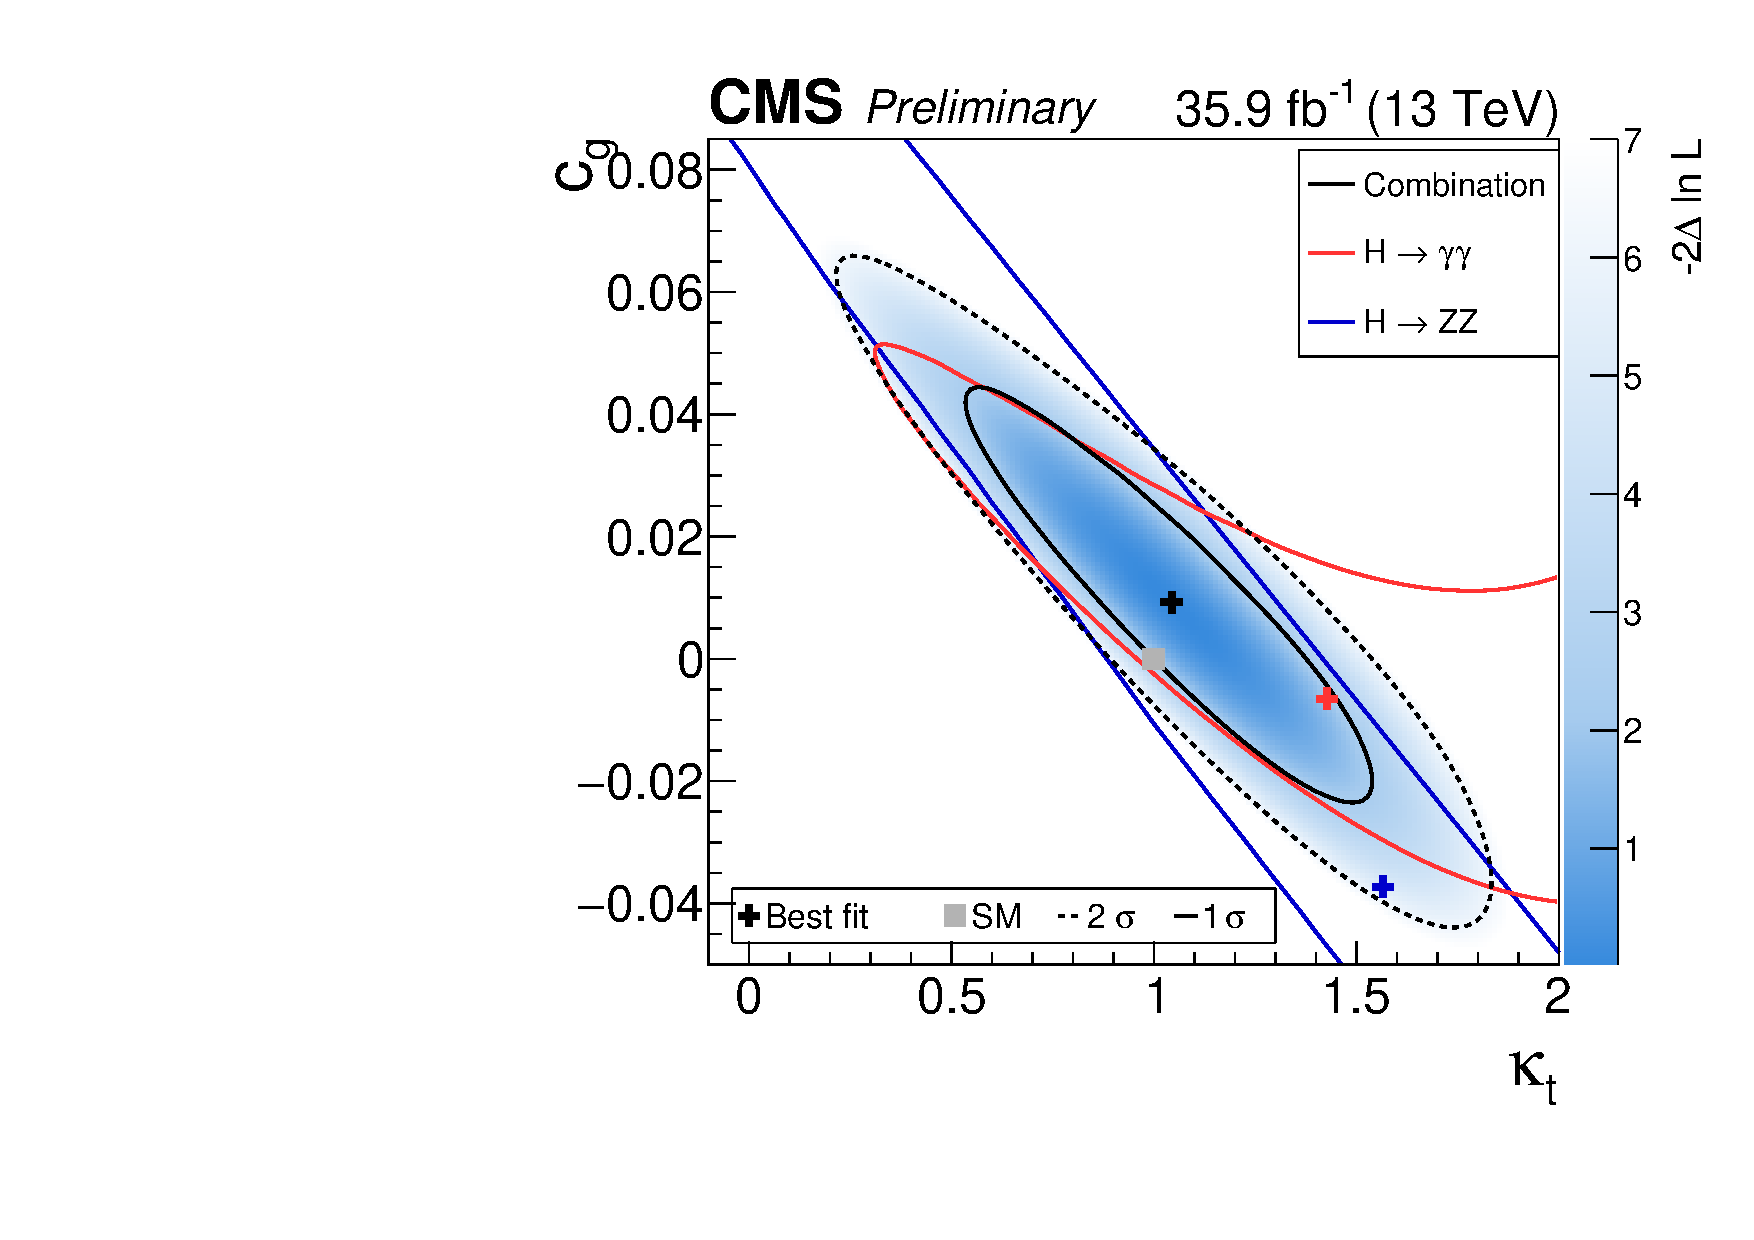
\includegraphics[width=0.49\linewidth]{img/resultsapproval/reworked/multicont_ktcg_couplingdependentBRs.pdf}
    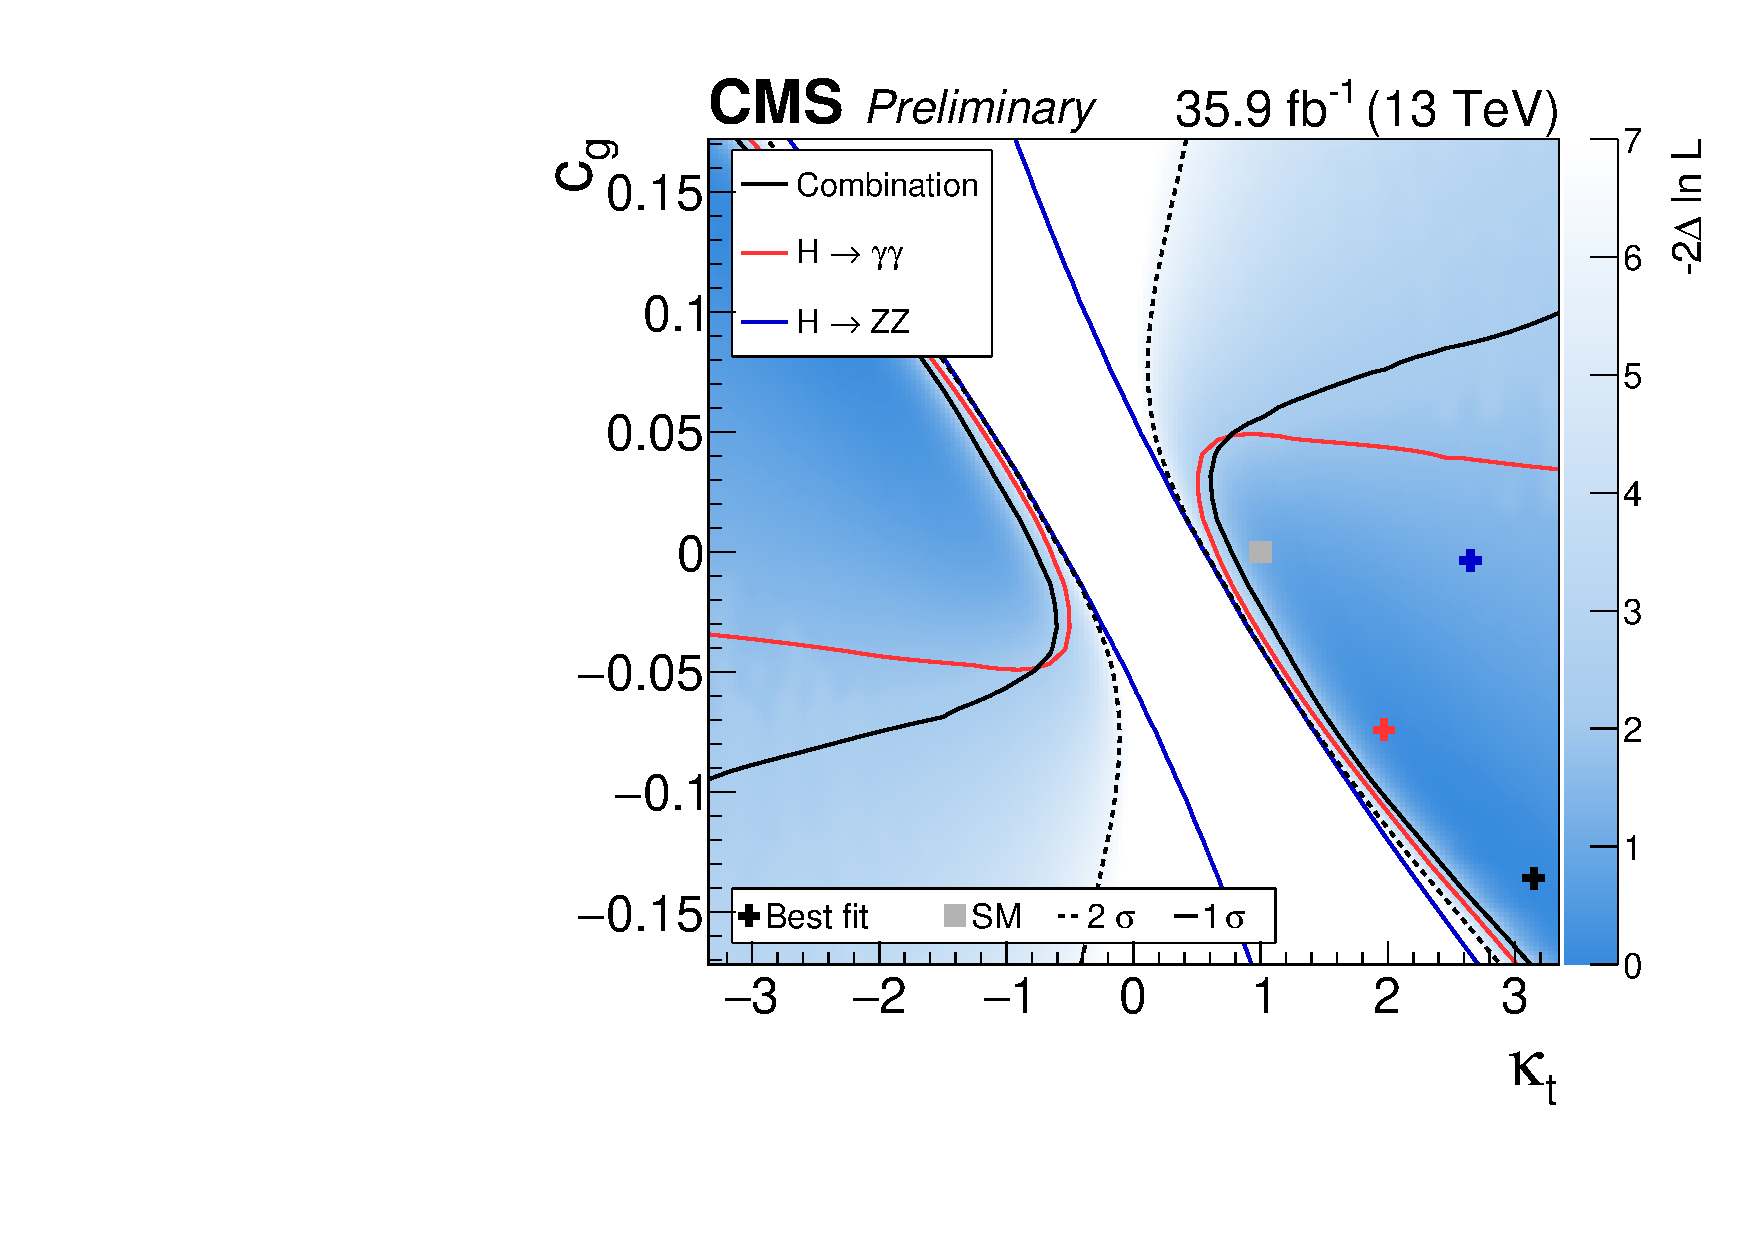
\includegraphics[width=0.49\linewidth]{img/resultsapproval/reworked/multicont_ktcg_floatingBRs.pdf}
    % 
    \caption{
        Simultaneous fit results for $\kappa_t$ and $\cg$.
        % 
        (\cmsLeft)
        % 
        One and two standard deviation contours are shown for the combined ($\hgg$, $\hzz$ and $\hbb$) fit to data and for $\hgg$ and $\hzz$ separately, assuming a coupling dependency of the branching fractions.
        % 
        % \arc{Fig.8 You don’t include Hbb alone because the uncertainty is too big ? How much is it ?}
        % \tk{Include $\hbb$-only}
        % 
        % (\cmsRight) The log-likelihood as a function of the angle in the $\kappa_t$-$\cg$ plane, letting the branching fractions float freely in the fit.
        % 
        (\cmsRight) One and two standard deviation contours are shown for the combined ($\hgg$, $\hzz$ and $\hbb$) fit to data and for $\hgg$ and $\hzz$ separately, assuming freely floating branching fractions.
        }
    \label{fig:scans_kappatkappag_nominal}
  \end{center}
\end{figure}


Figure~\ref{fig:scans_kappatkappab_rawInput}(\cmsLeft) shows the combined log-likelihood scan as a function of $\kappa_t$ and $\kappa_b$, with branching fractions scaling appropriately with the coupling modifiers and Figure~\ref{fig:scans_kappatkappab_rawInput}(\cmsRight) with freely floating branching fractions.
% 
As the $\hgg$ branching fraction depends linearly on $\kappa_t$, the constraints on $\hgg$ and the combination in Figure~\ref{fig:scans_kappatkappab_rawInput}(\cmsLeft) are not symmetric with respect to the $\kappa_t$-axis.
% 
For freely floating branching fractions, the parametrization is symmetric under $(\kappa_t,\,\kappa_b) \, \to \, (-\kappa_t,\,-\kappa_b)$, which explains the observed symmetry in in Figure~\ref{fig:scans_kappatkappab_rawInput}(\cmsRight).

\begin{figure}[hbtp]
  \begin{center}
    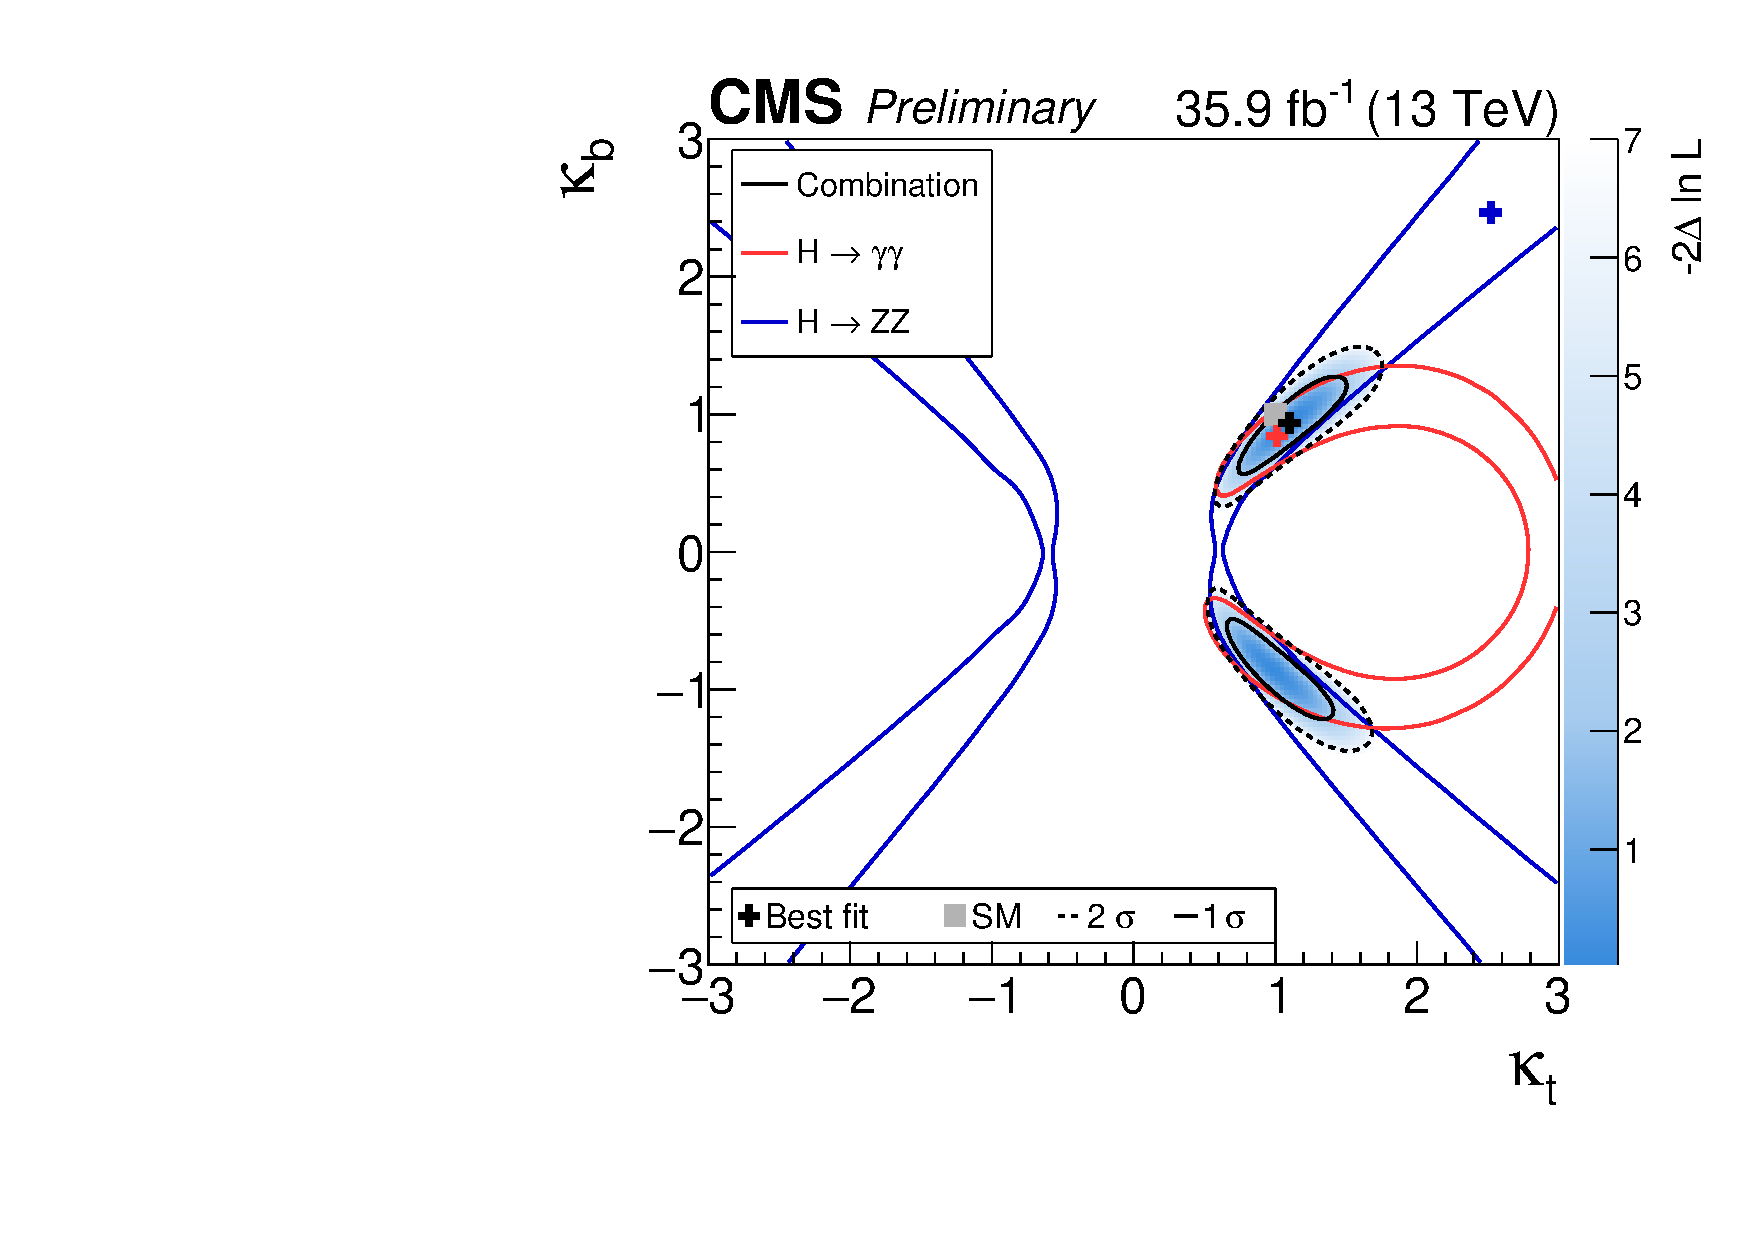
\includegraphics[width=0.49\linewidth]{img/resultsapproval/reworked/multicont_ktkb_couplingdependentBRs.pdf}
    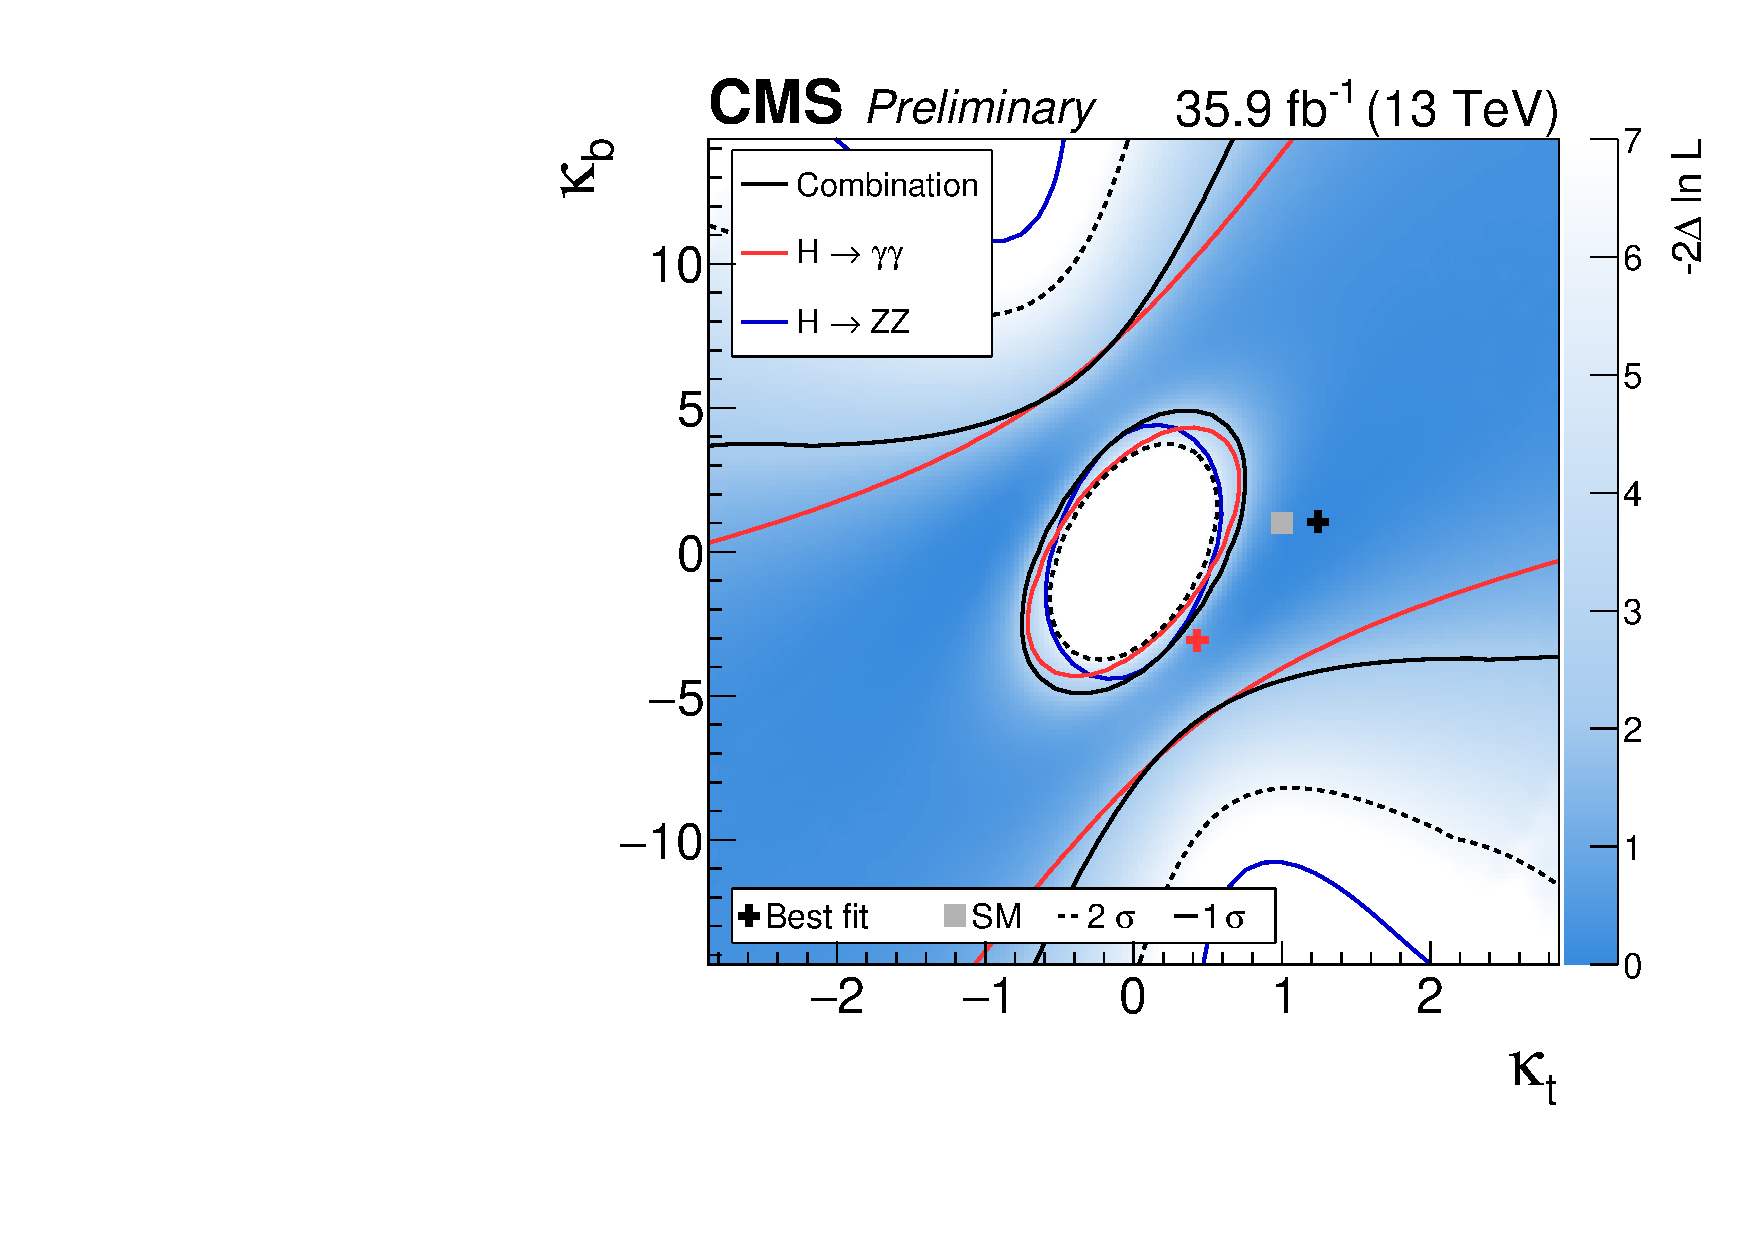
\includegraphics[width=0.49\linewidth]{img/resultsapproval/reworked/multicont_ktkb_floatingBRs.pdf}
    % 
    \caption{
        Simultaneous combined fit results for $\kappa_t$ and $\kappa_b$.
        % 
        (\cmsLeft) One and two standard deviation contours are shown for the combined ($\hgg$, $\hzz$ and $\hbb$) fit to data and for $\hgg$ and $\hzz$ separately, assuming a coupling dependency of the branching fractions.
        % 
        (\cmsRight) One and two standard deviation contours are shown for the combined ($\hgg$, $\hzz$ and $\hbb$) fit to data and for $\hgg$ and $\hzz$ separately, where the branching fractions were freely floated in the fit.
        }
    \label{fig:scans_kappatkappab_rawInput}
  \end{center}
\end{figure}




\toggledclearpage
\section{Conclusion}

A combination of differential cross sections for the differential observables $\pth$, $\njets$, $\absy$ and $\ptjet$ has been presented, using $35.9$\ifb of proton-proton collision data obtained at $\sqrt{s}=13$\TeV with the CMS detector.
% 
The spectra obtained are based on data from the $\hgg$, $\hzz$ and $\hbb$ decay channels.
% 
The overall uncertainty is decreased by 15\% relative to that for $\hgg$ alone by combining the $\pth$ spectra.
% 
The decrease is larger in the lower $\pth$ region than in the high $\pth$ tails.
% 
% An overall uncertainty decrease of uncertainty relative to $\hgg$ alone of about 15\% is realized with the combination of the $\pth$ spectrum, with a stronger improvement in the lower $\pth$ region than in the tails.
% 
No significant deviations from the SM are observed in any differential distribution.

The spectra obtained were interpreted in the Higgs coupling modifier framework, in which simultaneous variations of $\kappa_b$ and $\kappa_c$, $\kappa_t$ and $\kappa_g$ and $\kappa_t$ and $\kappa_b$ were fitted to the combination of the $\pth$-spectrum.
% 
The limits obtained on individual couplings were $\kappabLeftObserved < \kappa_b < \kappabRightObserved$ and $\kappacLeftObserved < \kappa_c < \kappacRightObserved$, assuming the branching fractions scale with the coupling modifiers.
% 
For the charm coupling $\kappa_c$ in particular, this measurement is competitive with those obtained from direct searches.

% Note a final \input at the bottom for the appendix (should decide if any is needed)

% ____________________________________________________________________________
\toggledclearpage

%% **DO NOT REMOVE BIBLIOGRAPHY**
\bibliography{auto_generated}   % will be created by the tdr script.

%% examples of appendices. **DO NOT PUT \end{document} at the end
\clearpage
\appendix

% ____________________________________________________________________________
\clearpage
\section{Correlation matrices for the combinations of differential observables}
\label{sec:binToBinCorrelationMatrices}

\begin{figure}[hbtp]
  \begin{center}
    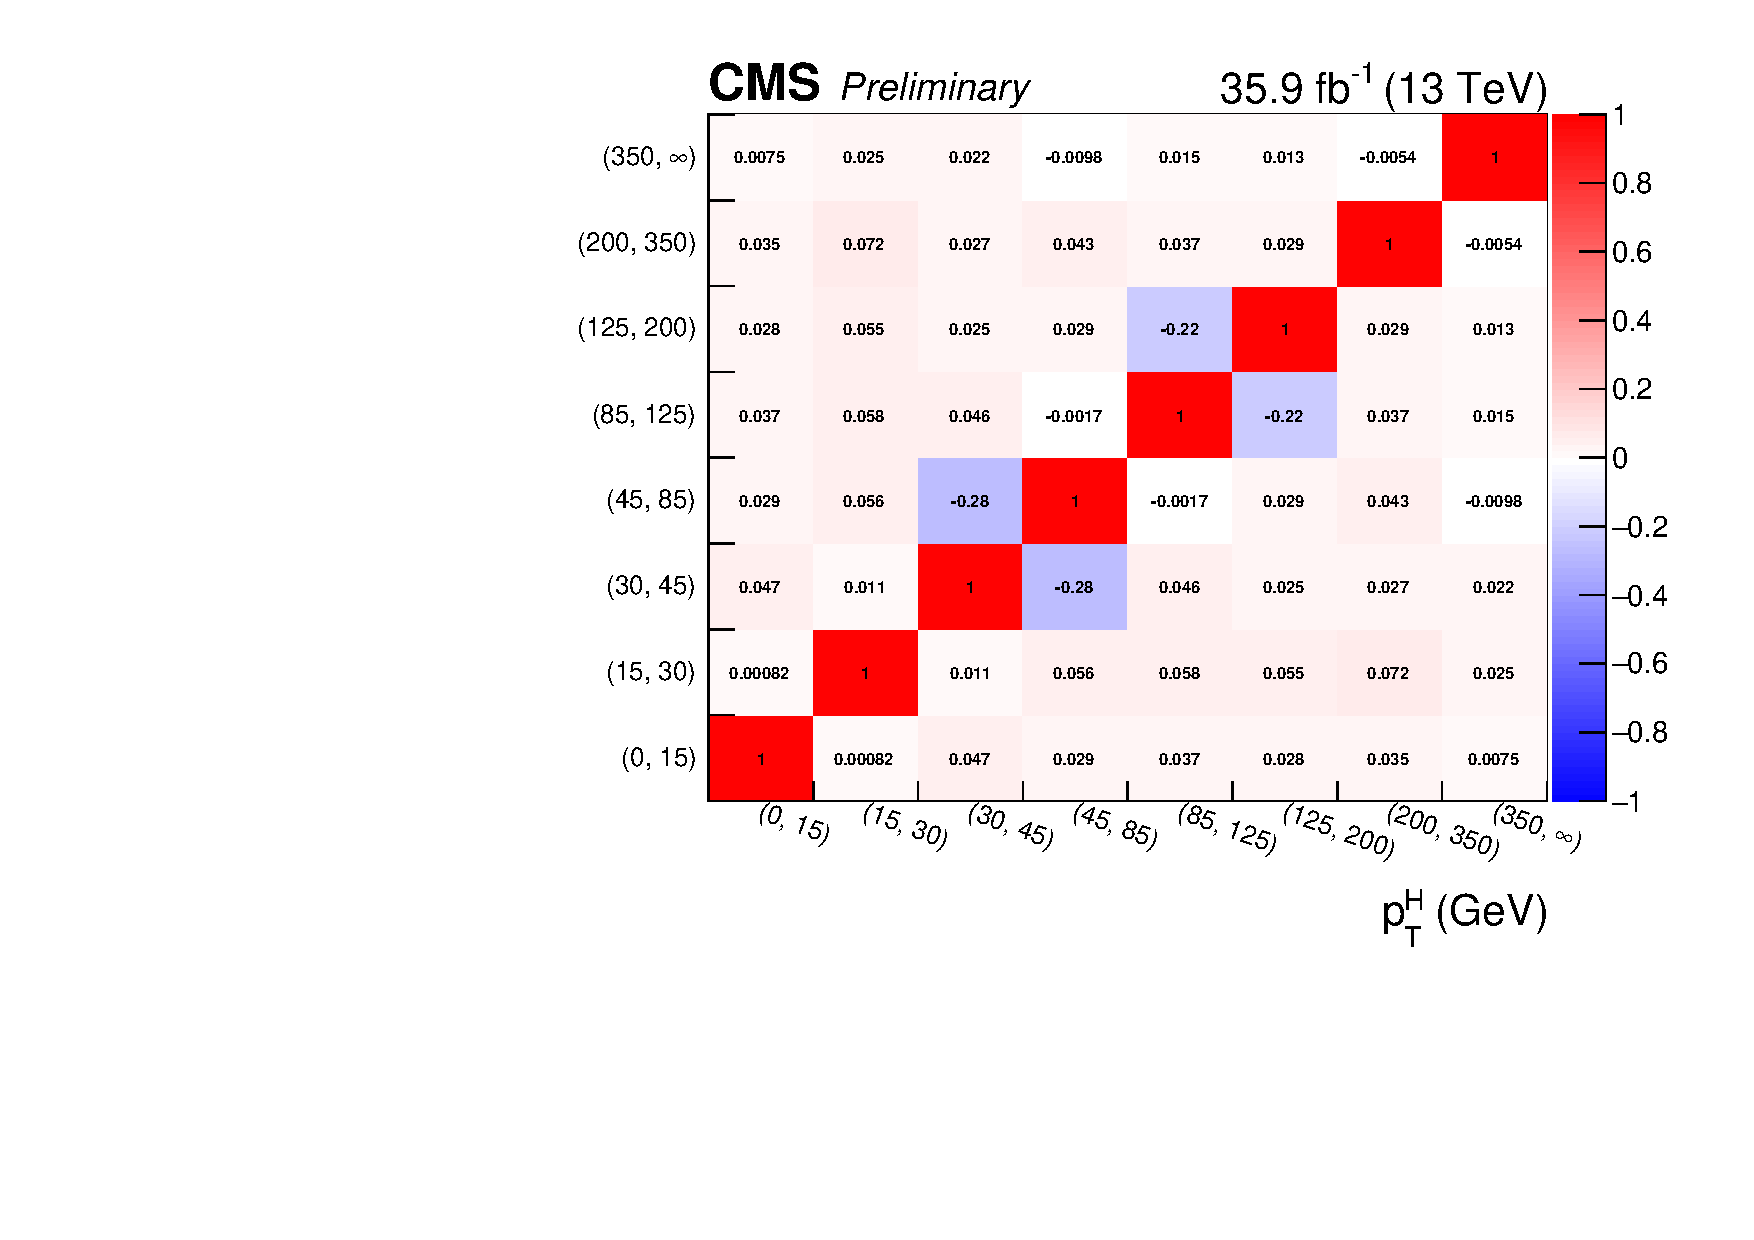
\includegraphics[width=\cmsFigWidth]{img/correlationMatrices/corrMat_CORRMAT_combinedCard_smH_Nov07_MultiDimFit_mH125.pdf}
    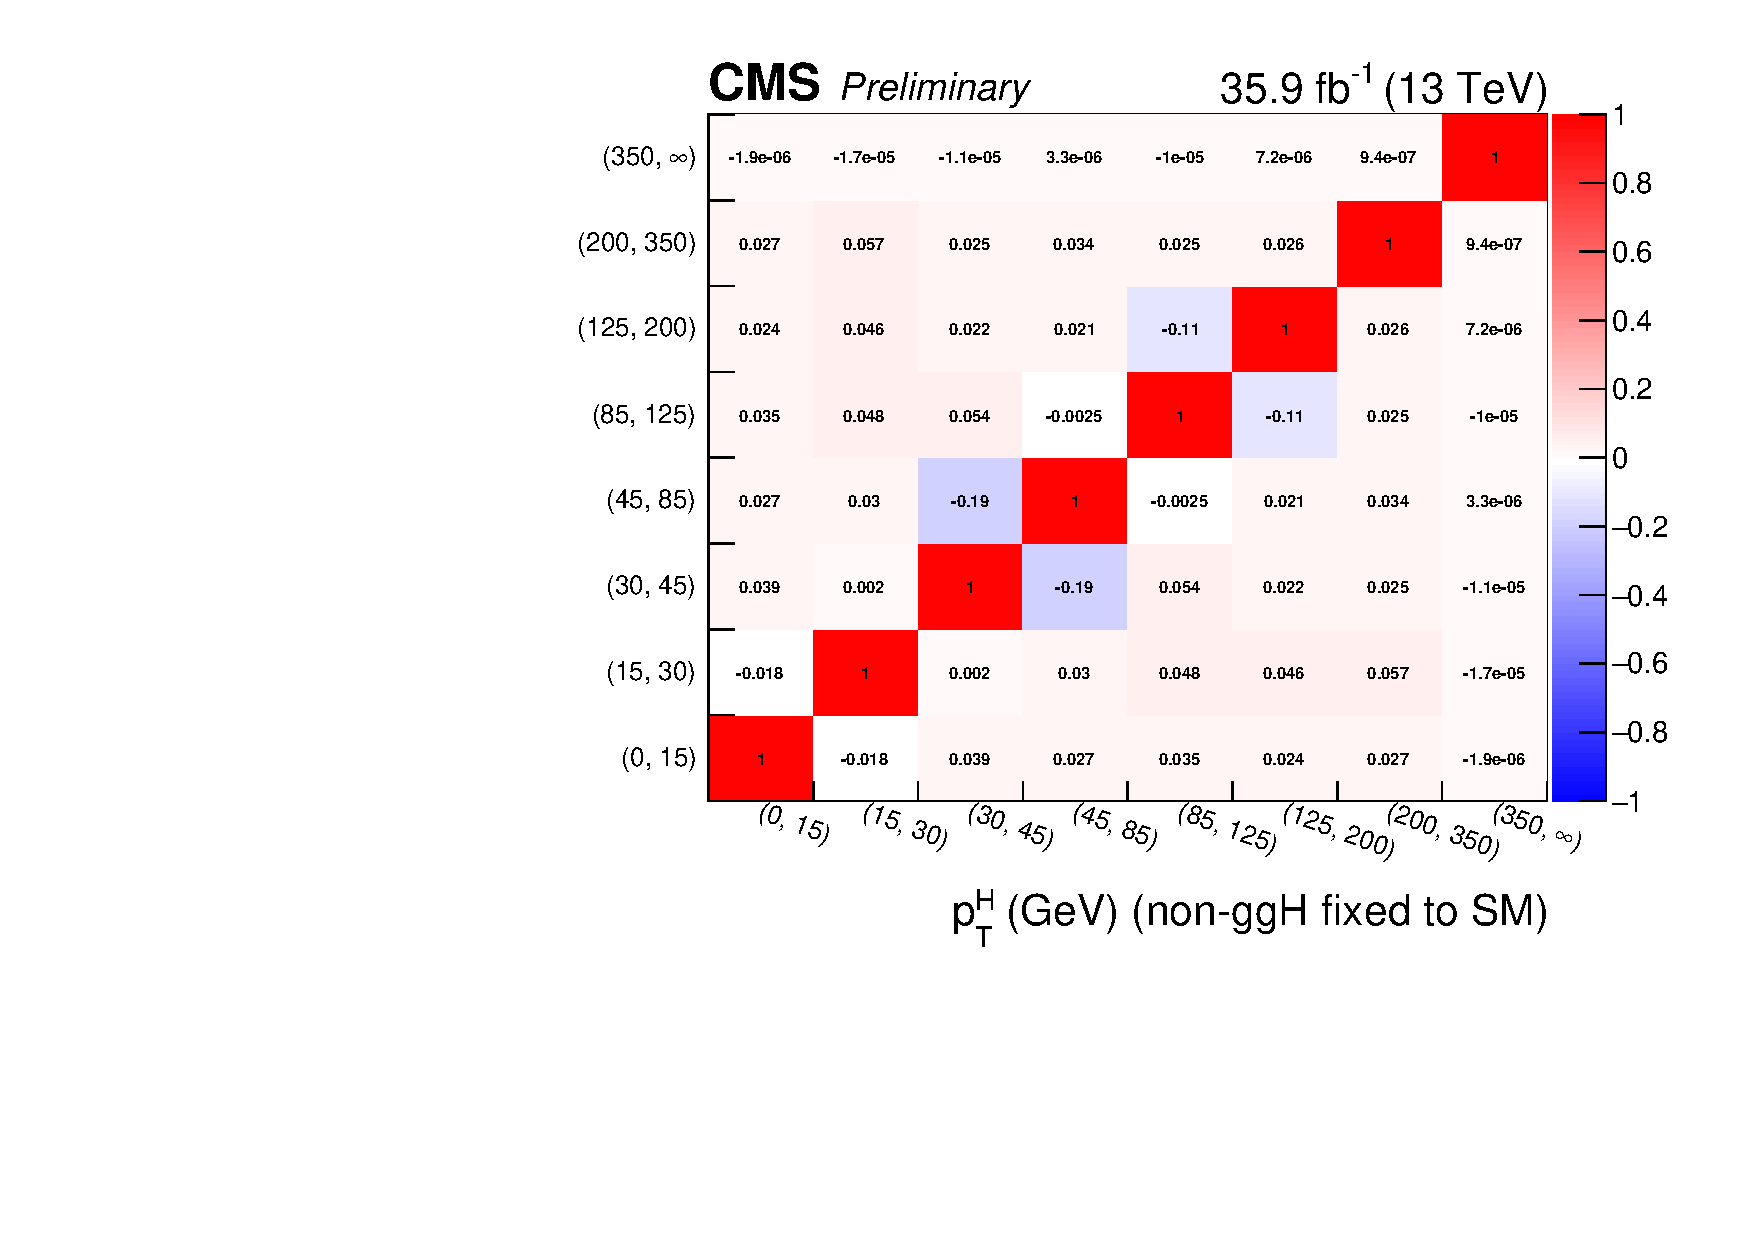
\includegraphics[width=\cmsFigWidth]{img/correlationMatrices/corrMat_CORRMAT_combinedCard_Nov03_xHfixed_MultiDimFit_mH125.pdf}
    \caption{
        (\cmsLeft) Bin-to-bin correlation matrix of the $\pth$-spectrum.
        (\cmsRight) Bin-to-bin correlation matrix of the $\pth$-spectrum, while keeping the non-gluon-fusion contributions (xH) fixed to SM expectation.
        }
    \label{fig:corrMat_pth}
  \end{center}
\end{figure}

\begin{figure}[hbtp]
  \begin{center}
    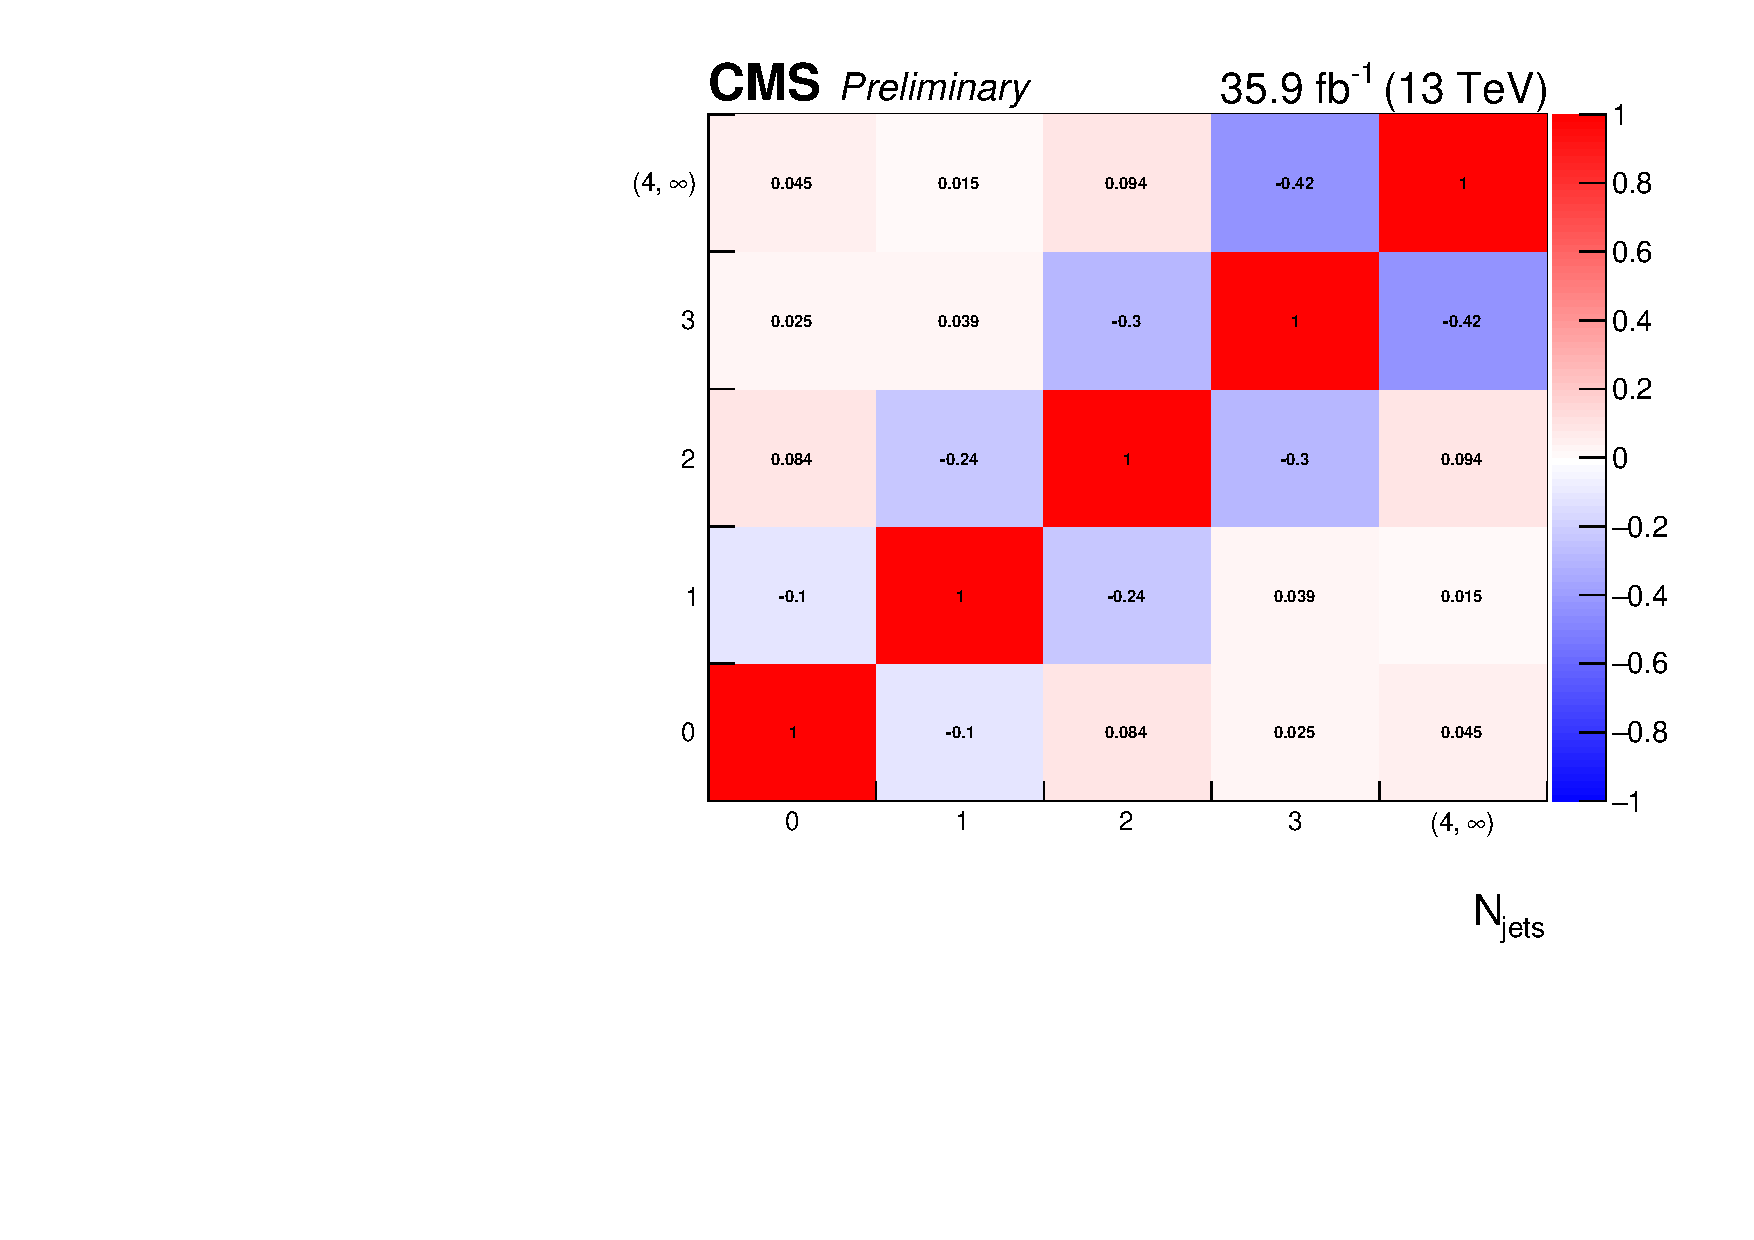
\includegraphics[width=\cmsFigWidth]{img/correlationMatrices/corrMat_CORRMAT_combinedCard_NJ_smH_Nov12_MultiDimFit_mH125.pdf}
    \caption{
        Bin-to-bin correlation matrix of the $\njets$-spectrum.
        }
    \label{fig:corrMat_njets}
  \end{center}
\end{figure}

\begin{figure}[hbtp]
  \begin{center}
    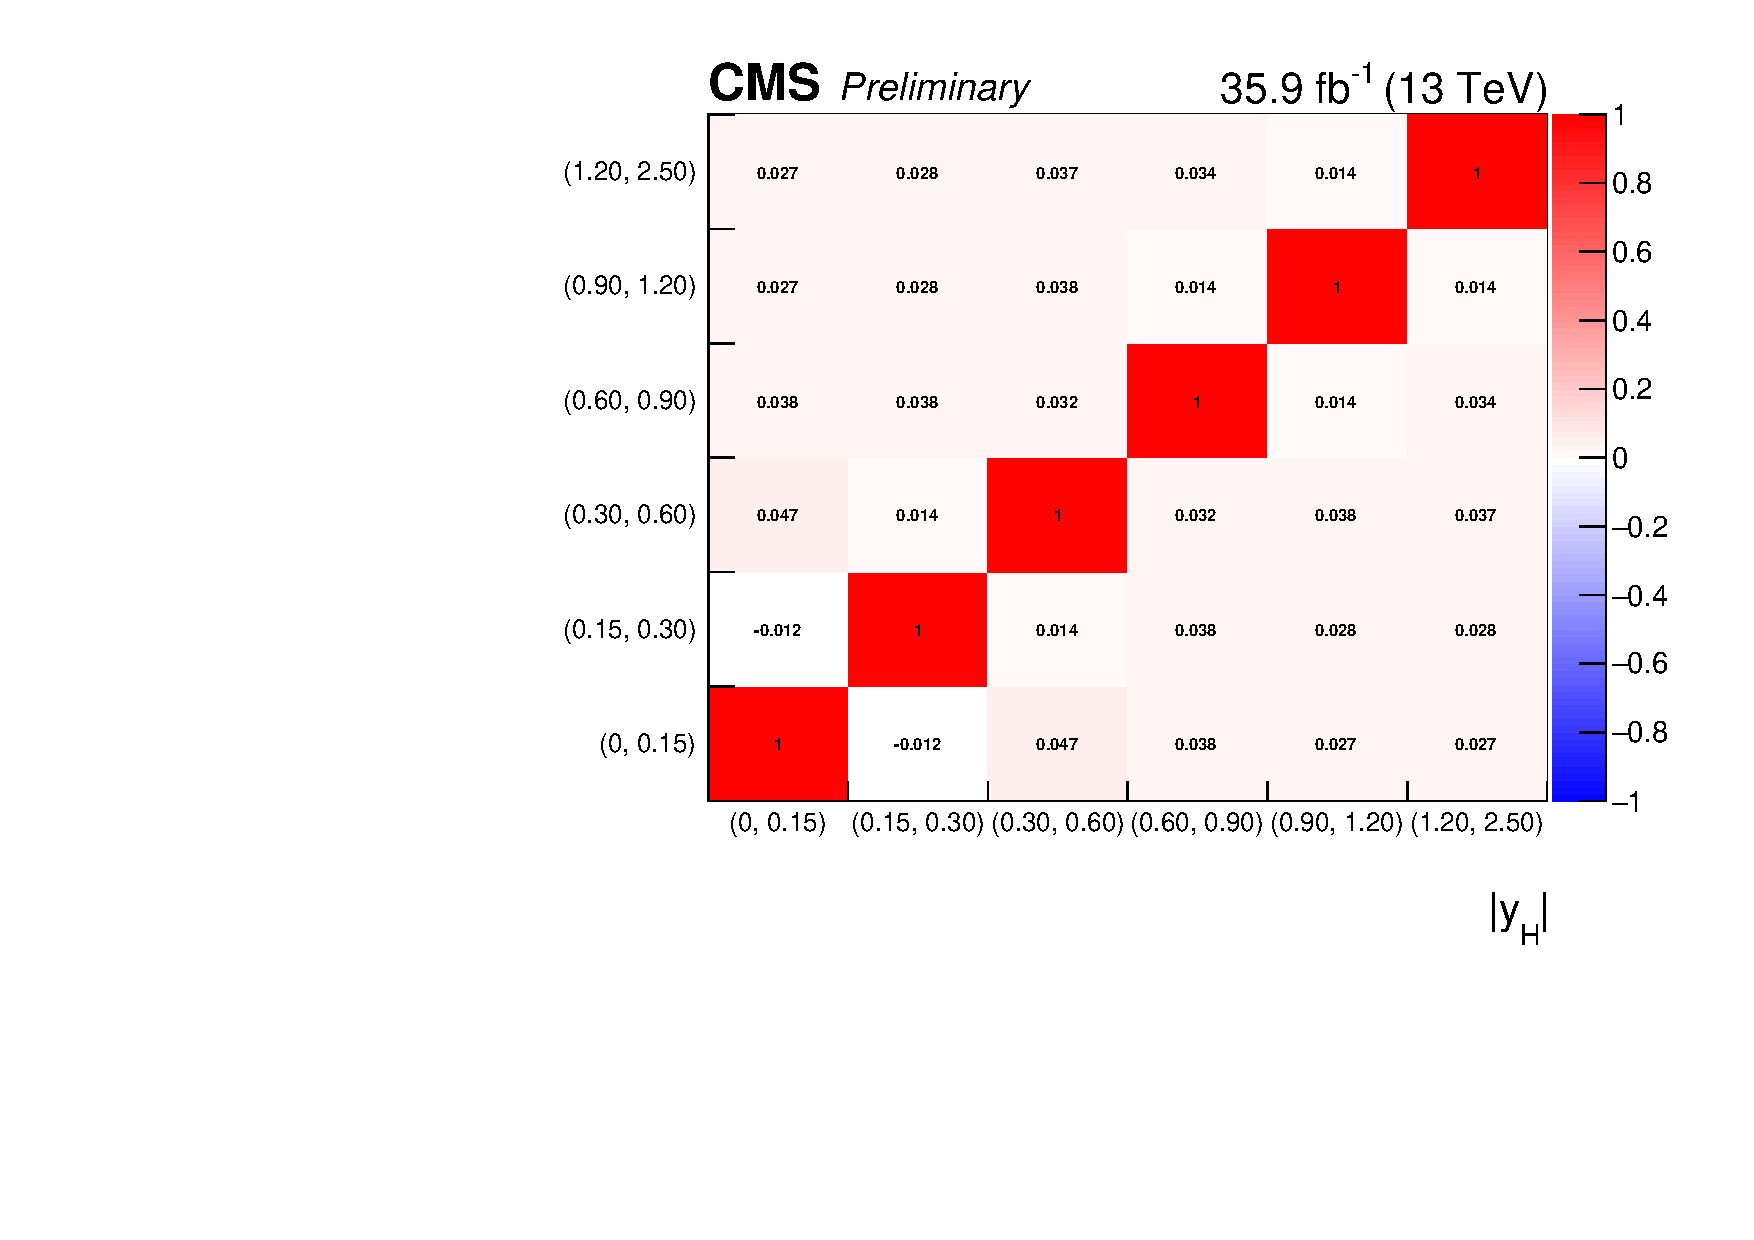
\includegraphics[width=\cmsFigWidth]{img/correlationMatrices/corrMat_CORRMAT_combinedCard_YH_smH_Nov28_MultiDimFit_mH125.pdf}
    \caption{
        Bin-to-bin correlation matrix of the $\absy$-spectrum.
        }
    \label{fig:corrMat_absy}
  \end{center}
\end{figure}

\begin{figure}[hbtp]
  \begin{center}
    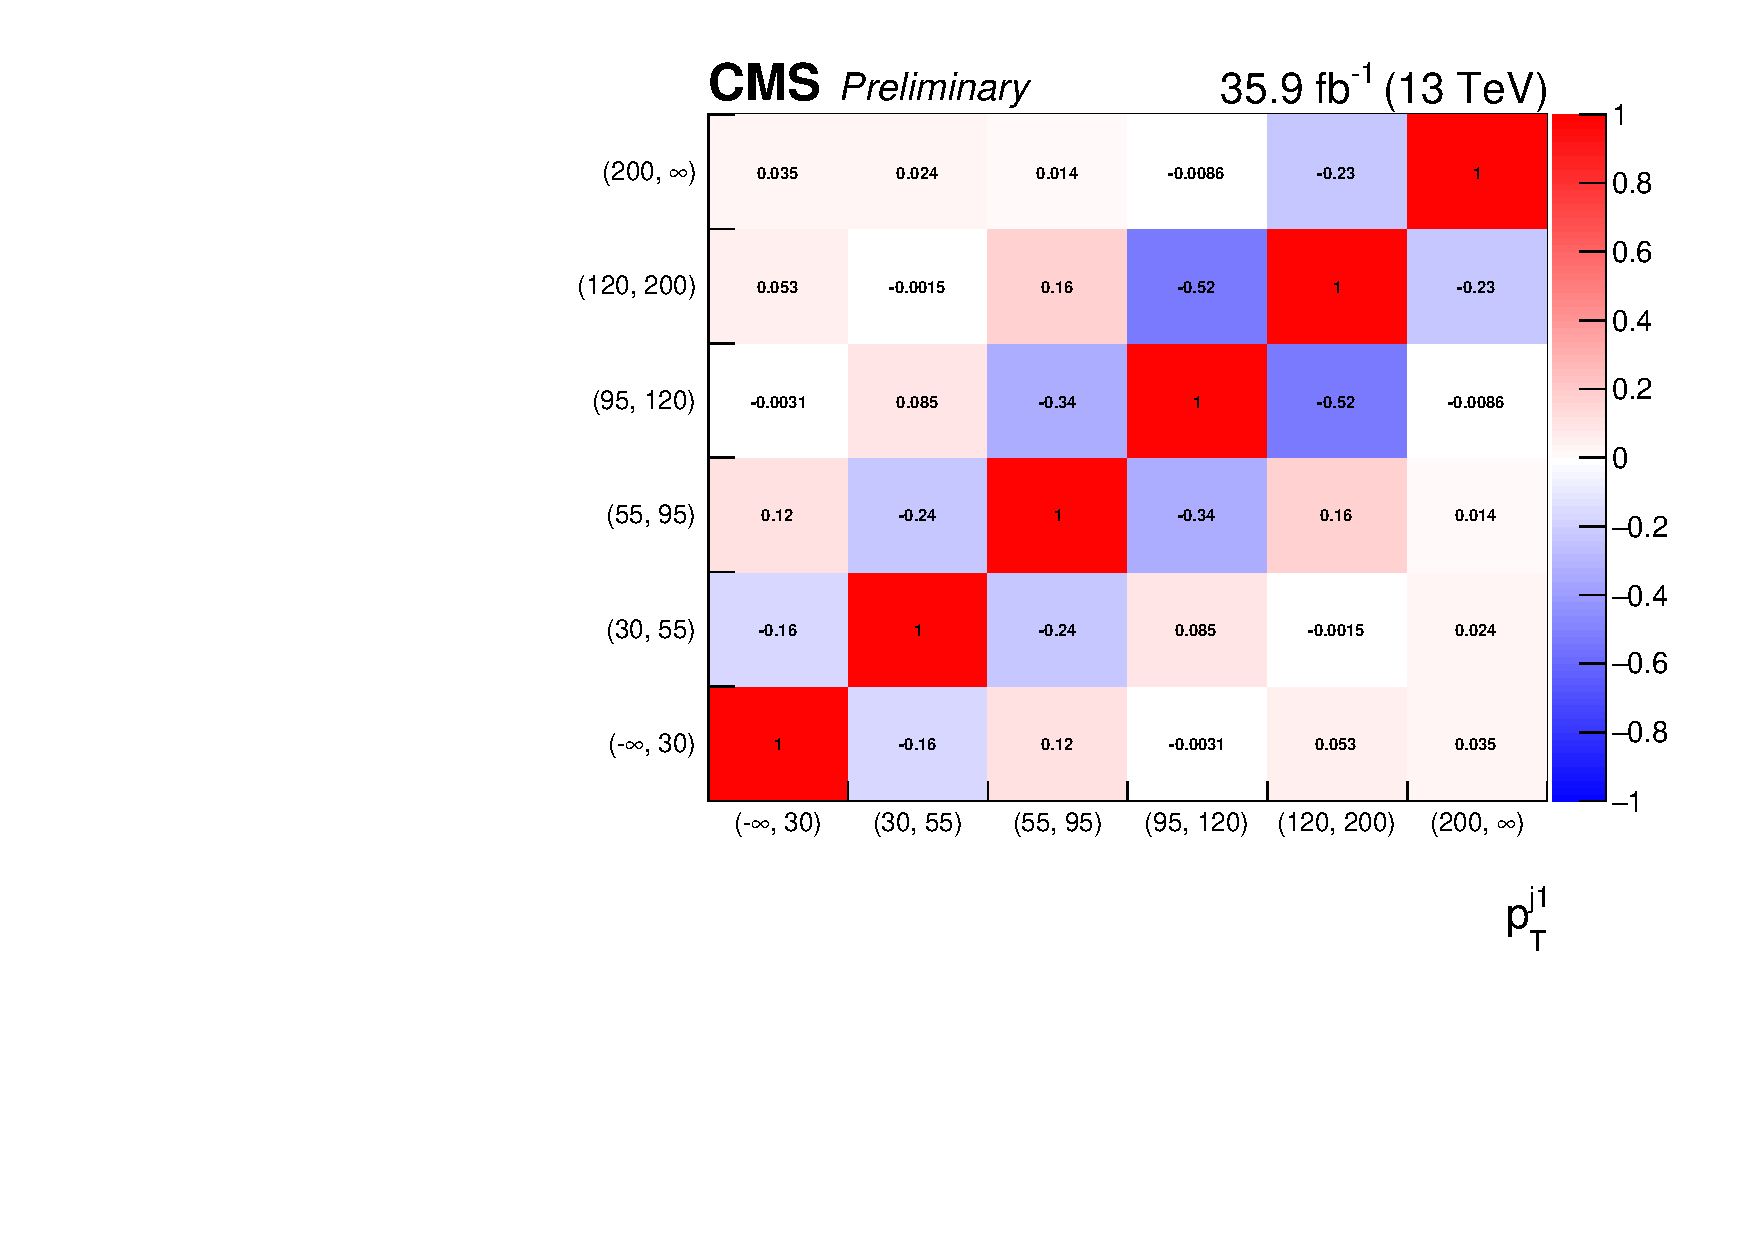
\includegraphics[width=\cmsFigWidth]{img/correlationMatrices/corrMat_CORRMAT_combinedCard_PTJ_smH_Nov28_MultiDimFit_mH125.pdf}
    \caption{
        Bin-to-bin correlation matrix of the $\ptjet$-spectrum.
        }
    \label{fig:corrMat_ptjet}
  \end{center}
\end{figure}

